\documentclass[a4paper,11pt,norsk]{article}

%Henter ulike pakker fra dokumentet packages.sty
\usepackage{packages}
\addbibresource{Bibliografi/bibliografi.bib}
\documentclass[tikz]{standalone}
\documentclass[11pt]{scrartcl} % use larger type; default would be 10pt
\usepackage[wby]{callouts}
\begin{document}

%Overskrift
%Headingdel:---------------------------------------------
\begin{minipage}[c]{0.15\textwidth}

\includegraphics[width=2.0cm]{Bilder/elsys_pos_staaende_ntnu.png}  
\end{minipage}
\begin{minipage}[c]{0.85\textwidth}

\renewcommand{\arraystretch}{1.7}
\large 
\begin{tabularx}{\textwidth}{|X|X|}
\hline
\multicolumn{2}{|l|}{\huge \textbf{TFE4172}} \\
\multicolumn{2}{|l|}{\huge \textbf{Grunnlag for}} \\
\multicolumn{2}{|l|}{\huge \textbf{faststoffelektronikk}} \\
\multicolumn{2}{|l|}{}  \\
\hline
\multicolumn{2}{|l|}{Tittel: 

%Skriv inn tittel her:------------------------------------------
Kompendium: TFE4172 Grunnlag for faststoffelektronikk (2024)
} \\
\hline
\multicolumn{2}{|l|}{Forfatter: 

%Skriv inn forfattere her:--------------------------------------
Haakon Alexander Hjul Strand
} \\
\hline

%Skriv inn versjon og dato her her:-----------------------------
Versjon: 1.0 & Dato: \today
\\
\hline 
\end{tabularx}
\end{minipage}
\normalsize

%Innholdfortegnelse
%Automatisk generert innholdsfortegnelse:------------------
\setlength{\parskip}{0ex}
\renewcommand{\baselinestretch}{0.1}\normalsize
\tableofcontents
\renewcommand{\baselinestretch}{1.00}\normalsize
\setlength{\parskip}{2ex}
\rule{\textwidth}{1pt}

%Selve rapporten:------------------------------------------
\section{Tema 1: Bølger og Bølgefunksjoner}
\label{tema1}
Dette er første samtale tema, det omfavner \textbf{prosjekt 1}. Dette inkluderer video forelesningene fra BB, se \textbf{tema 1}, \textbf{tema 2} og \textbf{tema 3}.

\autoref{tab:samtalePunkt_tema1} viser en tabell over samtale temaene, den inneholder en fargekode som representerer hvor godt jeg behersker samtaletemaet. \color{red}{Dårlig}, \color{blue}{ok, men ikke stabil} \color{black}{og} \color{teal}{Jeg er klar for eksamen}.

\color{black}
Målet er at alle temaene skal være grønne og dermed klar til eksamen.

\begin{table}[!htb]
    \centering
    \caption{Samtale punkter}
    \begin{tabular}{|c|c|c|r|}
      \hline
      1 & Ulike former for bølger &  \autoref{sec:tema1_1} & \cellcolor{blue}\quad\quad \\
      \hline 
      2 & Bølgeligningen i en dimenssjon & \autoref{sec:tema1_2} & \cellcolor{blue} \\
      \hline
      3 & Harmoniske bølger & \autoref{sec:tema1_3} & \cellcolor{blue} \\
      \hline
      4 & Stående bølger & \autoref{sec:tema1_4} & \cellcolor{green} \\
      \hline 
      5 & Bølgepakker & \autoref{sec:tema1_5} & \cellcolor{blue} \\
      \hline
      6 & Schrödingerligningen & \autoref{sec:tema1_6} & \cellcolor{green} \\ 
      \hline
      7 & Bølgefunksjonen & \autoref{sec:tema1_7} & \cellcolor{blue} \\
      \hline
      8 & Heisenbergs usikkerhets prinsipp & \autoref{sec:tema1_8} & \cellcolor{green} \\
      \hline
      9 & Dobbelspalte eksperimentet & \autoref{sec:tema1_9} & \cellcolor{green} \\
      \hline
    \end{tabular}
    \label{tab:samtalePunkt_tema1}
\end{table}

\subsection{Ulike former for bølger}
\label{sec:tema1_1}
En bølger er forstyrrelse som beveger seg eller \textbf{propagerer} vekk fra kilden, kilden i denne sammenhengen er systemet som produserer bølgen \cite{waves}. Bølger deles inn i to hovedkategorier; Mekaniske bølger og Elektromagnetiske bølger. Mekaniske bølger trenger et medium for å propagere, mens elektromagnetiske bølger ikke trenger et medium.


\begin{definition}
    \label{def:wave}
    Bølger transporterer energi uten å transportere masse.
\end{definition}

Eksempler på mekaniske bølger er bølger på en \textbf{streng}, \textbf{vannbølge} eller \textbf{lydbølge}. Fellesnevneren her er mediumet. For bølgen som beveger seg gjennom strengen er mediumet strengen selv, lydbølgen har luften som medium og vannbølgen har vannet.

Eksempler på elektromagnetiske bølger er \textbf{synlig lys}, \textbf{radiobølger} og \textbf{røntgenstråling}. Som nevnt over er ikke det ikke behov for et medium når en elektromagnetisk bølge beveger seg. Dette er fordi elektromagnetiske bølger består av osillerende elektriske og magnetiske felt, dette gjør at de kan propagere gjennom vakuum. \autoref{fig:bølgeTre} viser eksempler på bølger som inngår i hver hovedkategori.

\begin{figure}[!htb]
    \centering
    \includegraphics[scale=0.15]{Bilder/SamtaleTema1/BølgeFordeing.jpeg}
    \caption{Eksempel på bølger som som inngår i mekansike og elektromagnetiske bølger. Elektromagnetiske bølger har ingen longitudinale bølger}
    \label{fig:bølgeTre}
\end{figure}


\begin{definition}
\label{def:Transversale}
    \textbf{Transversale} bølger propagerer slik bølgemønsteret er vinkelrett på retningen til bølgen.
\end{definition}

\begin{definition}
\label{def:longitudinale}
    \textbf{Longitudiale} bølger beveger seg som bølger med sammentrykning. Longitudinale bølger beveger seg parallelt med retningen på propageringen.
\end{definition}

\begin{definition}
\label{def:ståendeBølge}
    \textbf{Stående bølger} er bølger der bølgemønsteret ser ut til å 'stå stille'.
\end{definition}

\autoref{fig:transversalBølge} viser hvordan en transversal bølge vil se ut, den blir i dette tilfellet produsert ved å bevege strengen vertikalt. Ved bruk av høyrehånden kan man se at dette skjer vinkelrett på bevegelsesretningen, la pekefinger peke i bevegelsesretning, og tommel peker opp i retningen av bølgemønsteret. \autoref{fig:longitudinalBølge} viser en longitudinal bølge, denne produseres ved å lage en horisontal bevegelse, den longitudinale bølgen beveger seg parallelt med bevegelsesretningen til bølgen. 

\begin{figure}[!htb]
    \centering
    \includegraphics[scale=0.7]{Bilder/SamtaleTema1/TransversaleBølge.png}
    \caption{Transversal bølge. \cite{waves}}
    \label{fig:transversalBølge}
\end{figure}


\begin{figure}[!htb]
    \centering
    \includegraphics[scale=0.7]{Bilder/SamtaleTema1/LongitudinalBølge.png}
    \caption{Longitudinal bølge. \cite{waves}}
    \label{fig:longitudinalBølge}
\end{figure}

Definisjon \ref{def:ståendeBølge} beskriver den stående bølgen, en stående bølge har det vi kaller noder, og antinoder. Noder er punktene som står stille i rommet, dvs de ikke har noe utslag. Antinoder er som navnet tilsier det motsatte av noder, dette er punktene som beveger seg mest, med andre ord utsvinget er størst. \autoref{fig:ståendeBølgeFig} viser tre stående bølger. Viktig ting å poengtere for stående bølger er at en stående bølge kun kan oppstå dersom begge sider er avgrenset, randbetingelsene for bevegesle i et eller begge ytterpunktene er null.

\begin{figure}[!htb]
    \centering
    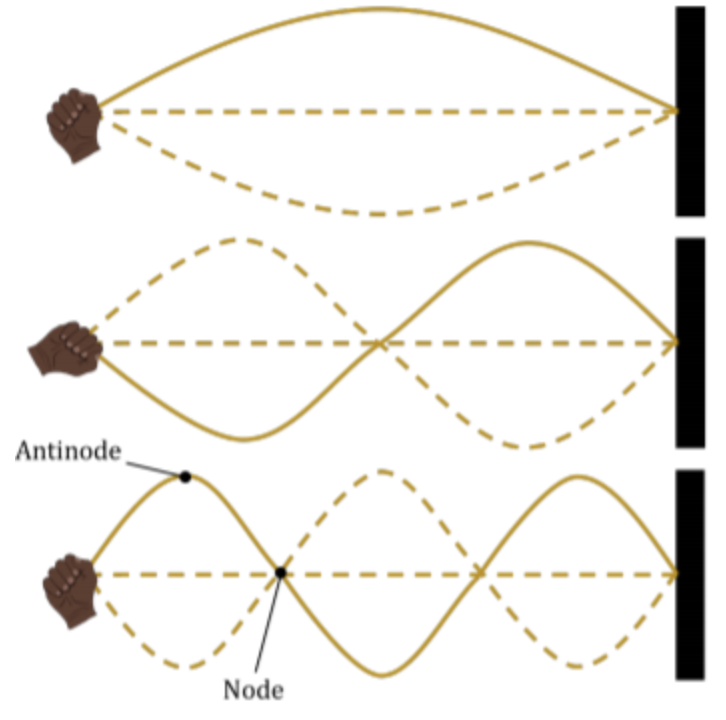
\includegraphics[scale=0.5]{Bilder/SamtaleTema1/sttåendeBølger.png}
    \caption{De tre første harmonene av stående bølger.}
    \label{fig:ståendeBølgeFig}
\end{figure}

\subsection{Bølgeligningen i en dimensjon}
\label{sec:tema1_2}
For å kunne beskrive bølgene som ble snakket om i \autoref{sec:tema1_1}, trenger man en matematisk modell som kan brukes til å beskrive og forstå bølgefenomener. Dette inkluderer lys, bølger på en streng osv. For å utlede bølgefunksjonen starter vi med å se på en enkel bølge. \autoref{fig:enkelBølge} viser en enkel sinus bølge, det røde rektangelet viser at vi ser nøye på en liten del av bølgen, dette er grunnlaget til skissen i figur \ref{fig:utledning_BL1D}, fremover blir bølgen refferert til som en streng.

\begin{figure}[!htb]
\begin{tikzpicture}
    \node[anchor=south west,inner sep=0] (image) at (0,0) {\includegraphics[width=0.9\textwidth]{Bilder/SamtaleTema1/bølgeDesmso.png}};
    \begin{scope}[x={(image.south east)},y={(image.north west)}]
        \draw[red,ultra thick,rounded corners] (0.6,0.55) rectangle (0.65,0.6);
    \end{scope}
\end{tikzpicture}
\caption{Enkel sinus bølge}
\label{fig:enkelBølge}
\end{figure}


\begin{figure}[!htb]
    \centering
    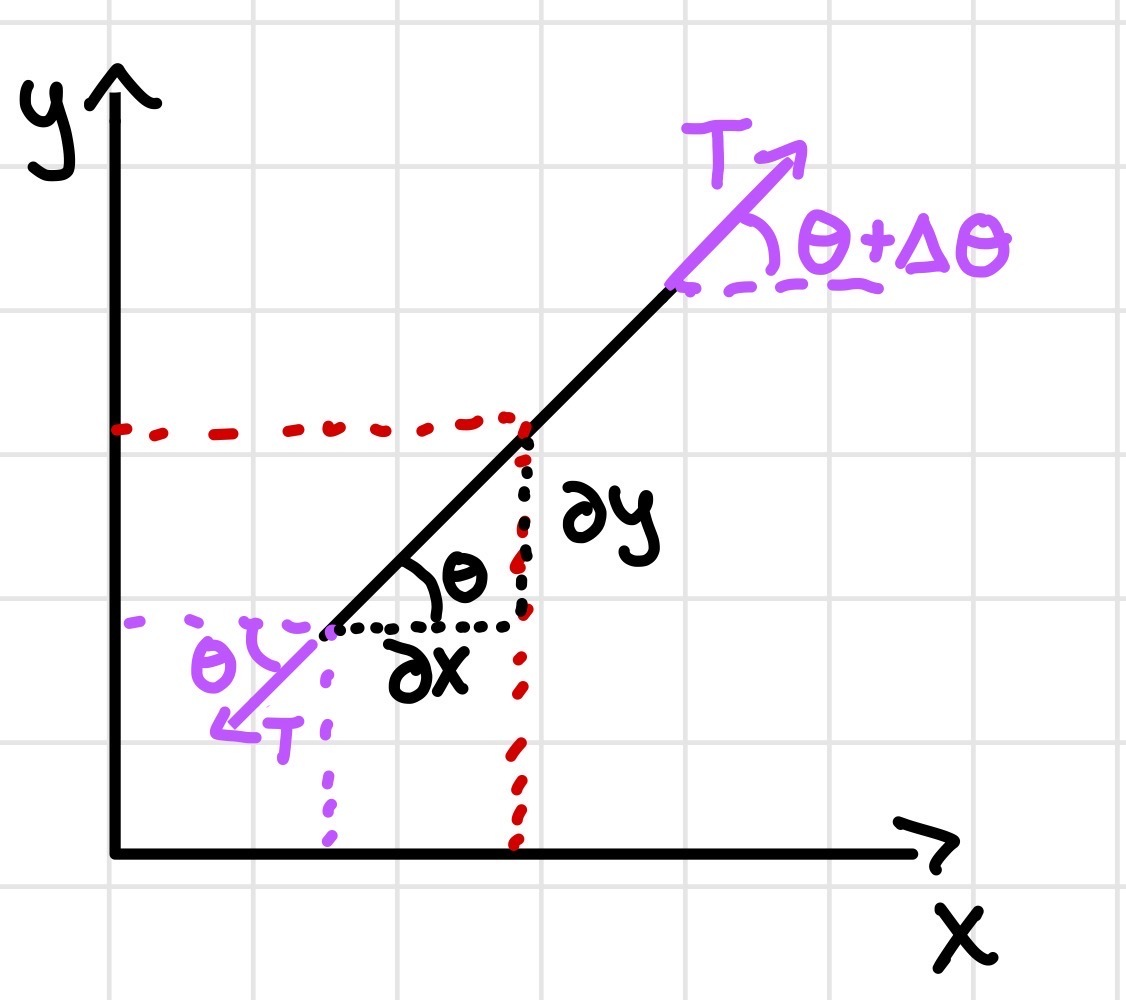
\includegraphics[scale=0.2]{Bilder/SamtaleTema1/utledning.jpeg}
    \caption{Utklipp av bølgen fra figur \ref{fig:enkelBølge}}
    \label{fig:utledning_BL1D}
\end{figure}

I tifellet fra figur \ref{fig:utledning_BL1D} er \color{red}T \color{black} snorkraften. Strengen har en masse, vi definerer denne som $\mu$ og har enhet $\bigg[\frac{kg}{m}\bigg]$. Vi kan si at delen av strengen vi ser på har lengde $\Delta x$, dermed er massen $m$.

\begin{equation}
    m = \mu \Delta x
\end{equation}

Vi ser på kreftene i y-retning, og tar i bruk småvinkel approksimasjon siden vi ser på et lite intervall.

\begin{equation}
    \begin{split}
        F_y &= -Tsin(\theta) + Tsin(\theta + \Delta)\\
        &\approx -T\theta + T\theta + T\Delta\theta
    \end{split}
\end{equation}

Siden $F=ma$, får vi at høyre side blir lik:

\begin{equation}
\label{eq:tema1_lhs}
    F_y = \mu \Delta x \frac{\partial^2y}{\partial t^2}
\end{equation}

og ved bruk at et triks\footnote{$tan(\theta)=\frac{\partial y}{\partial x} \implies$ deriver mhp. x og bruk småvinkelapproximasjon $\implies \Delta \theta =\Delta x \frac{\partial^2 y}{\partial x^2}$} kan vi skrive høyresiden

\begin{equation}
\label{eq:tema1_rhs}
    F_y = T \Delta x \frac{\partial^2y}{\partial x^2}
\end{equation}

Setter vi sammen ligning \ref{eq:tema1_lhs} og ligning \ref{eq:tema1_rhs} får vi

\begin{equation}
\label{eq:variantBL1D}
    \frac{\mu}{T} \frac{\partial^2 y}{\partial t^2} = \frac{\partial^2 y}{\partial x^2}
\end{equation}

\autoref{eq:variantBL1D} er en variant av bølgeligningen, generelt er $f(x \pm ct) $ en løsning på bølgeligningen, der $c = \sqrt{\frac{T}{\mu}}$, $c$ har dermed benevning $\big[\frac{m}{s}\big]$. Dette representerer farten til bølgen. Derfor er det vanligere å bruke $v$ istedet for $c$, da det er mer generelt og c brukes ofte for lysfarten (farten til elektromagnetiske bølger i vakum). Med det får man den mer generelle formen på den endimensjonale bølgeligningen sett i ligning \ref{eq:BL1D}.

\begin{empheq}[box=\tcbhighmath]{align}
    \label{eq:BL1D}
    \frac{1}{v^2} \frac{\partial^2 y}{\partial t^2} = \frac{\partial^2 y}{\partial x^2}
\end{empheq}

Dersom utledningen har litt hull og ikke gir full forståelse, se denne videoen \MYhref{https://www.youtube.com/watch?v=ub7lok-JQJE}{Bølgeligningen i 1D for nybegynnere}.


\newpage
\subsection{Harmoniske bølger}
\label{sec:tema1_3}
Den enkleste bølgen er den harmoniske bølgen (eller sinusbølge)\footnote{I tilfellet for osillatorer og bølger er disse synonymer.} Harmoniske bølger får man på formen vist i ligning \ref{eq:harmonicEQ}.

\begin{empheq}[box=\tcbhighmath]{align}
    \label{eq:harmonicEQ}
    u(x,t) = A\cdot cos(kx - \omega t + \phi)
\end{empheq}

En bølge har en periode, en periode $T$ er definert som tiden det tar fra et punkt på bølgen 'gjentar' seg. Bølgelengden $\lambda$ til en bølge er definert som avstanden i meter mellom to ekvivalente punkt eller med andre ord avstanden på en periode $T$. I tilfellet for ligning \ref{eq:harmonicEQ} er $k$ bølgetallet, og har et invers proporsjonalt forhold med bølgelengden, $k=\frac{2\pi}{\lambda} = [\frac{1}{m}]$. $f$ er frekvensen til bølgen, $f=\frac{1}{T}=[\frac{1}{s}]$ og kan tenkes på som hvor mange ganger i sekundet bølgen kommer med samme informasjon. $\omega$ er vinkelfrekvensen, denne er proporsjonal med frekvensen til bølgen, $\omega = 2\pi f = [\frac{rad}{s}]$. $\phi$ er faseforskyvningen til bølgen, dvs. hvor mye bølgen har blitt ''dyttet'' fra sin originale startverdi. Sist men ikke minst har vi amplituden til bølgen, siden $cos(...)$ kun innehar verdier som oppfyller ulikheten $| cos(...)|<1$, må vi ha noe som påvirker amplituden, dette er $A$, $A$ er en konstant\footnote{Dersom man vil legge til f.eks en dempningsfaktor kan man gange den harmoniske bølgen med en eksponentsialfunksjon $e^{-t\alpha}$ der alpha er en dempningskonstant.}.

Formalisme mtp. hvordan man skriver bølgefunksjonen er valgfritt, dersom man velger å bruke sinus er det snakk om et faseskift på $\frac{\pi}{2}$. Dersom $\phi$ er negativ ser det ut som bølgen forskyves mot høyre (dersom de andre verdiene i bølgen er negative). så vi kan dermed si at $sin(x) = cos(x -\frac{\pi}{2})$.

Når man skal regne med sinuser og cosinuser kan det bli vanskelig og man må ha god kontroll på trigonometriske identiteter for å kunne forenkle uttrykk. Det finnes heldigvis en annen måtte å regne på bølger, dette er ved bruk av \textbf{Eulers formel} som vi ser i ligning \ref{eq:euluers}.

\begin{equation}
    \label{eq:euluers}
    e^{i\alpha} = cos(\alpha) + isin(\alpha)
\end{equation}

Ved bruk av ligning \ref{eq:harmonicEQ} og ligning \ref{eq:euluers} kan vi skrive om uttrykket vi har for harmoniske bølger og vi får ligning \ref{eq:omskrivningHarmonic}

\begin{empheq}[box=\tcbhighmath]{align}
    \label{eq:omskrivningHarmonic}
    Acos(kx-\omega t + \phi) = \Re\bigg(Ae^{i(kx-\omega t + \phi}\bigg)
\end{empheq}

Siden vi som oftest jobber med klassiske bølger dropper vi $\Re$, dette er fordi den klassiske harmoniske bølgen ikke inneholder noen imaginære bidrag.
\newpage
\subsubsection{Gruppe- og Fasehastighet}
\textbf{Gruppehastighet} er hastigheten til en bølgepakke som beveger seg gjennom et medium. 
\begin{equation}
    \label{eq:gruppv}
    v_g = \frac{\partial \omega}{\partial k}
\end{equation}

\textbf{Fasehastigheten} til en bølge er ''rate at which the wave propogates in any medium.'', 

\begin{equation}
    \label{eq:fasev}
    v_p = \frac{\lambda}{T} = \frac{\omega}{k}
\end{equation}
Bruk gjerne animasjonene fra \MYhref{https://en.wikipedia.org/wiki/Group_velocity}{Wikipedia} for visualisering av konseptet, for en harmonisk bølge er disse to like.
\subsubsection{Viser regning}
Dette er tilleggsmateriell og ikke helt nødvendig for pensumet i faget (anno. 2024). 

En viser er en representasjon av en sinusformet bølge med amplitude, A, fasekonstant, $\phi$, og vinkelfrekvens, $\omega$, er uavhengig av tid (tidinvariant). Tidsinvariansen gir oss følgende definisjon:

\begin{equation}
    \label{eq:viser}
    Asin(\omega t +\phi) = \Re\bigg(Ae^{i\phi}e^{i\omega t}\bigg)
\end{equation}

Vi kan her si at $\textbf{v} = Ae^{i\phi}$ er viseren, denne ''spinner'' rundt i det komplekse plan som en funksjon av tid. selvom viseren ikke har en tidsvariabel er dette en metafor for å hjelpe på forståelsen av viseren. $\textbf{V}$ er et imaginært tall som inneholder informasjon om amplituden og fase vinkelen til den gitte sinus funksjonen \cite{EC10th}. \autoref{fig:viserPlot} er en illustrasjon som skal vise hva som har blitt skrevet i dette avsnittet, dette er vanskelig så se gjerne på fler ressurser på internett for bedre forklaringer.

\begin{figure}[!htb]
    \centering
    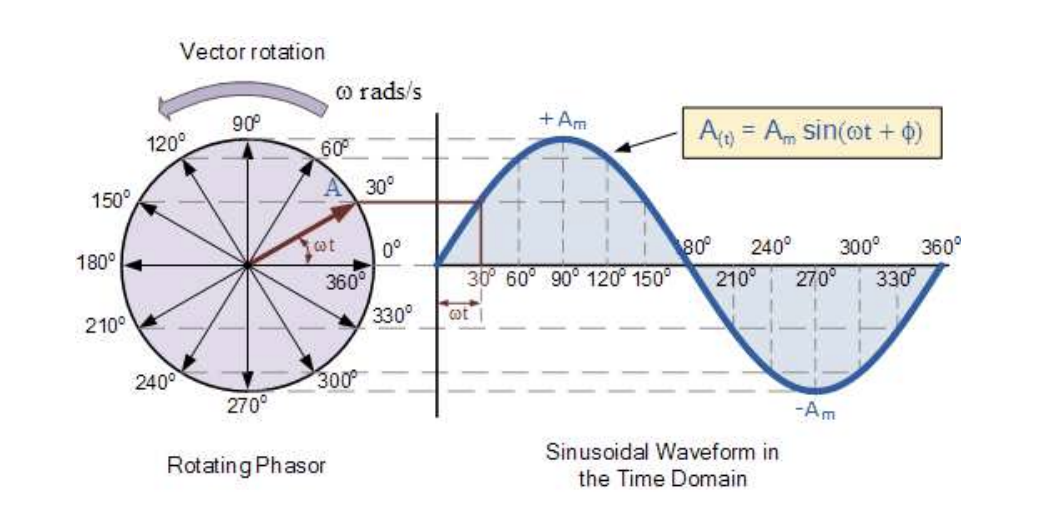
\includegraphics[scale=0.7]{Bilder/SamtaleTema1/viser.png}
    \caption{Henter fra Electronics tutorials \cite{electronics}.}
    \label{fig:viserPlot}
\end{figure}


\newpage
\subsection{Stående bølger}
\label{sec:tema1_4}
Vi skal legge litt mer informasjon til i definisjonen vår av stående bølger fra \autoref{sec:tema1_1}. Vi kan definere en stående bølge som vi har gjort i definisjon \autoref{def:ståendeBølge}, men vi kan også definere det som definisjon \autoref{def:ståendeBølge2}.

\begin{definition}
    \label{def:ståendeBølge2}
    Kombinasjon av to bølger som beveger seg i \textbf{motsatte} retninger. Begge har samme amplitude og frekvens
\end{definition}

En konsekvens av informasjoen fra definisjon \ref{def:ståendeBølge2} er at bølger som ''kolliderer'' med hverandre vil gi opphav til fenomenet interferens, dette gjør at superposisjnen av bølgene vil enten øke den totale bølgeamplituden eller minke den, hhv. konstruktiv og destruktiv interferens. 

Vi tar et eksempel, la oss si vi har to bølger, de er definert i ligning \ref{eq:u1} og ligning \ref{eq:u2}.

\begin{equation}
    \label{eq:u1}
    u_1(x,t) = Acos(kx+\omega t)
\end{equation}
\begin{equation}
    \label{eq:u2}
    u_2(x,t) = Acos(kx-\omega t)
\end{equation}

Vi ser at ligning \ref{eq:u1} og \ref{eq:u2} har to bølger som beveger seg likt i rommet, men ulikt i tid. Dersom vi tar i bruk superposisjonsprinsippet kan vi si at summen av de energien fra de to bølgene er det den totale påvirkningen på omgivelsene.

\begin{equation}
    \label{eq:superpos}
    \begin{split}
        u(x,t) &= u_1(x,t) + u_2(x,t)\\
        &= Acos(kx+\omega t) + Acos(kx-\omega t)\\
        &= 2A cos(kx) cos(\omega t)
    \end{split}
\end{equation}

Resulatet fra \autoref{eq:superpos} produserer en bølge vi kaller en stående bølge, denne består av en bølge $cos(kx)$, denne varierer i rom, og vi har $cos(\omega t)$ som vil variere i tid.

\begin{gather*}
    \begin{split}
    &\text{Avstand mellom to noder: $\frac{\lambda}{2}$}\\
    &\text{Avstand mellom node og antinode: $\frac{\lambda}{4}$}
    \end{split}
\end{gather*}

For en stående bølge er det ingen energitransport, et annet vanlig navn for denne type bølge er ''Stasjonær bølge''.
\newpage

\subsection{Bølgepakker}
\label{sec:tema1_5}
En bølgepakke er en sammensatt bølge, pakken består da av en superposisjons av bølger, dvs:

\begin{equation}
    U(x,t) = \Sigma_{k=1}^N u_k(x,t)
\end{equation}

Bølgepakken vil bevege seg med gruppehastigheten til bølgen $v_g$. Dersom to forskjellige bølger er løsninger på bølgeligningen (\ref{eq:BL1D}), vil summen av de to også løse ligning \ref{eq:BL1D}. Dersom systemene ikke er lineære stemmer ikke dette, en enkel forklaring på dette er at addering er en lineær operasjon.

\subsection{Schrödingerligningen}
\label{sec:tema1_6}
De-Broglie postulerte i sin PhD oppgave fra 1924 at akkurat som lys hadde både partikkel og bølge egenskaper. Ville elektroner også ha bølge egenskaper. Resulatet mot slutten av PhD oppgaven er dette kjente uttrykket: 

\begin{equation}
    \label{eq:debroglie1}
    \lambda = \frac{h}{p}
\end{equation}

\autoref{eq:debroglie1} inneholder informasjon om partikkelens bølgelengde $\lambda$, og bevegelseslmengde $p$. Plancks konstant $h$ innehar omtrent verdien $6.63\cdot10^{-34}\,\si{\joule\per\second}$. Uttrykket kan skrives om til ligning \ref{eq:debroglie2} ved bruk av $k=\frac{2\pi}{\lambda}$ og $\hbar = \frac{h}{2\pi}$.

\begin{equation}
    \label{eq:debroglie2}
    p = \hbar k
\end{equation}

Ved å si at partikkeler har bølge egenskaper kan vi skrive om engergien ved hjelp av frekvensen, akkurat som for lys.

\begin{equation}
    \label{eq:energy}
    E = hf = \frac{h\omega}{2\pi}=\hbar\omega
\end{equation}

Vi må beskrive bølgene våre også, vi tar i bruk det vi så på i \autoref{sec:tema1_3} om harmoniske bølger, og vi skriver derfor en 3D bølge slik som i ligning \ref{eq:bølgefunc3D}

\begin{equation}
    \label{eq:bølgefunc3D}
    \Psi(\textbf{r},t) = e^{i(\textbf{k}\textbf{r}-\omega t)}
\end{equation}

I en dimensjon skriver vi det som i ligning \ref{eq:bølgefunc1D}
\begin{empheq}[box=\tcbhighmath]{align}
    \label{eq:bølgefunc1D}
    \Psi(x,t) = e^{i(kx -\omega t)}
\end{empheq}

I 1925 postulerte shrödinger en ligning utifra hva De-Broglie hadde funnet om ''materie bølgen''. Han kom fram til ligning \ref{eq:shrodinger}

\begin{empheq}[box=\tcbhighmath]{align}
    \label{eq:shrodinger}
    i\hbar \frac{\partial \Psi}{\partial t} = \hat{H}\Psi
\end{empheq}

Her er $\Psi$ bølgefunksjonen som ble beskrevet i ligning \ref{eq:bølgefunc1D}. Ved bruk av shrodinger ligningen kan man finne en rekke verdier som forklarer en bølge $\Psi$ er en bølgefunksjon som løser shrödiner ligningen. Vi kan bruke det som et eksempel til å finne bevegelsesmengden $p$, men for å finne $p$ må vi anvende en operator. $p=\hbar k$, så hvis vi deriverer $\Psi$ mhp $x$ er vi et steg nærmere.

\begin{equation}
    \frac{\partial}{\partial x}\Psi(x,t) = ik \cdot e^{i(kx-\omega t)}
\end{equation}

Vi er et steg nærmere ja, men vi har en $i$ her og vi mangle $\hbar$, så la oss modifisere operatoren så den ganger med $\hbar$ og deler på $i$.

\begin{equation}
    \frac{\hbar}{i}\frac{\partial}{\partial x}\Psi(x,t) = \hbar k \Psi(x,t) = p\Psi(x,t)
\end{equation}

Vi får ved bruk av operatoren $\hat{P}$ ut $p$, her er $p$ en reell tallverdi. Når en operator anvendt på en bølgefunksjon 'stemmer' sier vi at $\Psi(x,t)$ er en egentilstand av $\hat{P}$ med egenverdi $p$.

\begin{empheq}[box=\tcbhighmath]{align}
    \label{eq:bevegelsesmengdeOperator}
    \hat{P} = \frac{\hbar}{i} \frac{\partial}{\partial x}
\end{empheq}

Vi kan gjøre det samme for energien, vi vet at den kan bli skrevet på formen som ligning \ref{eq:energy}. Vi får dermed at 

\begin{equation}
    \begin{split}
    i\hbar \frac{\partial}{\partial t} \Psi(x,t) &= i \hbar (-i\omega)\Psi(x,t) \\
    &= \hbar \omega \Psi(x,t) \\
    &= E\Psi(x,t)
    \end{split}
\end{equation}

Dette er strengt tatt riktig, men vi vil fange at energien kan skrives ved bruk av bevegelsesmengden $p$ og massen $m$ til partikkelen, vi tar derfor i bruk forholdet sett i ligning \ref{eq:energy2}.

\begin{equation}
    \label{eq:energy2}
    E = \frac{p^2}{2m}
\end{equation}

Vi ønsker med det å lage en operator vi kaller $\hat{O}$ som henter ut denne informasjonen fra bølgefunksjonen. Vi starter med å utledning:

\begin{equation}
    \label{eq:utledning_energi}
    \begin{split}
        \hat{O}\Psi &= \frac{p^2}{2m}\Psi \\
        &= \frac{p}{2m}\cdot(p\Psi) \\
        &= \frac{p}{2m}\cdot(\frac{\hbar}{i}\frac{\partial}{\partial x}\Psi) \\
        &= -\frac{\hbar^2}{2m}\frac{\partial^2}{\partial x^2}\Psi
    \end{split}
\end{equation}

Vi ser nå at operatoren vi kalte $\hat{O}$ like gjerne kan bli kalt $\hat{E}$ da den henter ut energien fra bølgen, på den måten vi ville ha den. Det er viktig å skille mellom operatoren vi nettop fant og den Hamiltonske operatoren $\hat{H}$. De er begge energi operatorer, men $\hat{E}$ har med en fri partikkel å gjøre, mens $\hat{H}$ inneholder informasjon om potensialet partikkelen befinner seg i. Den Hamiltonske operatoren blir nyttig når vi ser på partikkel i brønn og videre. Med det i bakhodet har vi schrödingers ligning for frie partikler i ligning \ref{eq:shrodinger_freeparticle}

\begin{empheq}[box=\tcbhighmath]{align}
    \label{eq:shrodinger_freeparticle}
    i\hbar \frac{\partial}{\partial t} \Psi = -\frac{\hbar^2}{2m}\frac{\partial^2}{\partial x^2}\Psi
\end{empheq}

og SL ved bruk av den Hamiltonske operatoren skrevet ut:

\begin{empheq}[box=\tcbhighmath]{align}
\label{eq:shrodinger_boundedparticle}
\begin{split}
    i\hbar \frac{\partial}{\partial t} \Psi(x,&t) = \bigg(-\frac{\hbar^2}{2m}\frac{\partial^2}{\partial x^2} + V(x,t)\bigg)\Psi(x,t)\\
    &i\hbar \frac{\partial}{\partial t} \Psi(x,t) = \hat{H}\Psi(x,t)
\end{split}
\end{empheq}

\autoref{eq:shrodinger_boundedparticle} viser den fullstendige Shrödinger ligningen.

\subsubsection{Tidsuavhengige S.E (TISE)}
Det er vanskelig og komplekst å jobbe i tid og rom samtidig, derfor vil vi prøve å se om vi kan forenkle Shrödinger ligningen. Vi prøver derfor å separere rom og tid med produktløsning (separable variabler)

\begin{equation}
    \label{eq:separableVariable}
    \Psi(x,t) = \psi(x)T(t)
\end{equation}

Vi setter ligning \ref{eq:separableVariable} inn i SL og deler med $\Psi$ på begge sider

\begin{equation}
    \label{eq:bevis_1}
    \frac{i\hbar}{T}\frac{\partial T}{\partial t} = \frac{1}{\psi} \hat{H}\psi
\end{equation}

Vi ser at høyre og venstre side er like, selv om venstre side kun er avhengig av tid og høyre er avhengig av rom. Vi kan skrive om ligning \ref{eq:bevis_1} og løse for T:

\begin{equation}
    \label{eq:T(t)}
    \begin{split}
        \frac{dT}{T} &= \frac{E}{i\hbar}dt \\
        \int\frac{dT}{T} &= \int\frac{E}{i\hbar}dt\\
        ln(T(t)) &= \frac{Et}{i\hbar} \\
        T(t) &= e^{\frac{-iEt}{\hbar}}
    \end{split}
\end{equation}

Vi kan nå sette dette inn igjen i ligning \ref{eq:separableVariable} og prøve å løse SL.

\begin{equation}
    \label{eq:stasjonær}
    \Psi(x,t) = \psi(x)e^{\frac{-iEt}{\hbar}}
\end{equation}

\autoref{eq:stasjonær} kalles en stasjonær tilstand, dette er fordi sannsynlighetstettheten er uavhenging av tiden $t$\footnote{$|\Psi(x,t)|^2 = |\psi(x)|^2$, fordi $|e^{i\beta}|^2 = 1$, auvhengig av verdien til $\beta$.}.

\begin{equation}
    \label{eq:TISE}
\begin{split}
    i\hbar\frac{\partial}{\partial t} \psi(x)e^{-\frac{i(\hbar\omega)t}{\hbar}} &= 
    \bigg[ 
    -\frac{\hbar^2}{2m} \frac{\partial^2}{\partial x^2} + V(x)
    \bigg] \psi)e^{-\frac{i(\hbar\omega)t}{\hbar}}\\
    \hbar\omega\psi(x) \highlight{e^{-\frac{i(\hbar\omega)t}{\hbar}}} &=
    \bigg[ 
    -\frac{\hbar^2}{2m} \frac{\partial^2}{\partial x^2} + V(x)
    \bigg] \psi)\highlight{e^{-\frac{i(\hbar\omega)t}{\hbar}}} \\
    E\psi(x) &= \hat{H}\psi(x)
\end{split}
\end{equation}

\autoref{eq:TISE} viser oss at ved bruk av separable variabler, kan vi få SL til å være tidsuavhengig. Den tidsuavhengige Shrödinger ligningen vil ha diskrete egenverdier og/eller kontinuerlige energibånd.

\subsection{Bølgefunksjonen}
\label{sec:tema1_7}
Bølgefunksjonen $\Psi$ må være kompleks, dette gjør at $\Psi$ ikke er en direkte målbar fysisk størrelse. $\Psi$ er proporsjonal med intensiten $I$, dette brukte Max Born til å finne et forhold for sannsynligheten til et partikkel mhp. posisjon.

\begin{equation}
\label{eq:born}
    dp = |\Psi(x,t)|^2dx
\end{equation}

\autoref{eq:born} gir et uttrykk for sannsynligheten for å finne partikkelen mellom $x$ og $x + dx$ ved en tid $t$. Vi vet nå at sannsynligheten til å finne en partikkel er direkte korelert med bølgefunksjonen $\Psi$, integrerer vi opp alle sannsynlighetsbidragene får vi såklart $1$. Så dersom vi har en fri partikkel som kan befinne seg hvor som helst på en linje på intervallet $[-\infty,\infty]$ får vi:

\begin{equation}
    \label{eq:normalisering}
    \int_{-\infty}^{\infty} |\Psi(x,t)|^2 = 1
\end{equation}

\subsection{Heisenbergs usikkerhets prinsipp}
\label{sec:tema1_8}
En konsekvens av kvantemekanikken er Heisenbergs usikkerhets prinsipp (HUP), siden bølgefunksjonen ikke sier noe om absolutt posisjon, men noe om sannsynligheten til at partikkelen er et sted ved obsersvasjon. Så må det ligge en usikkerhet i hva vi kan måle. Det gir ikke mening i kvantemekanikken å snakke om en presis bestemmelse av både posisjon og bevegelsesmengde. 

\begin{empheq}[box=\tcbhighmath]{align}
\label{eq:HUP}
    \Delta x \Delta p \leq \frac{\hbar}{2}
\end{empheq}

\autoref{eq:HUP} viser HUP, For HUP er notasjonen med $\Delta$ det samme som standard avvik, så $\Delta x = \sigma_x$. 

Vi ser at en ren sinus bølge, som den i figur \ref{fig:enkelBølge} har en gitt frekvens. Når vi har frekvens kan vi være veldig sikre på energien til bølgen, siden $p=\hbar \omega$, men det er umulig å si noe om posisjonen. Om vi legger sammen mange forskjellige bølger til det oppstår en kompakt bølgepakke, kan vi si noe om posisjonen, men det blir umulig å si noe om energien til bølgen uten å vite hva den er bygget opp av. \autoref{fig:prosjekt1_eksempel}

\begin{figure}[!htb]
    \centering
    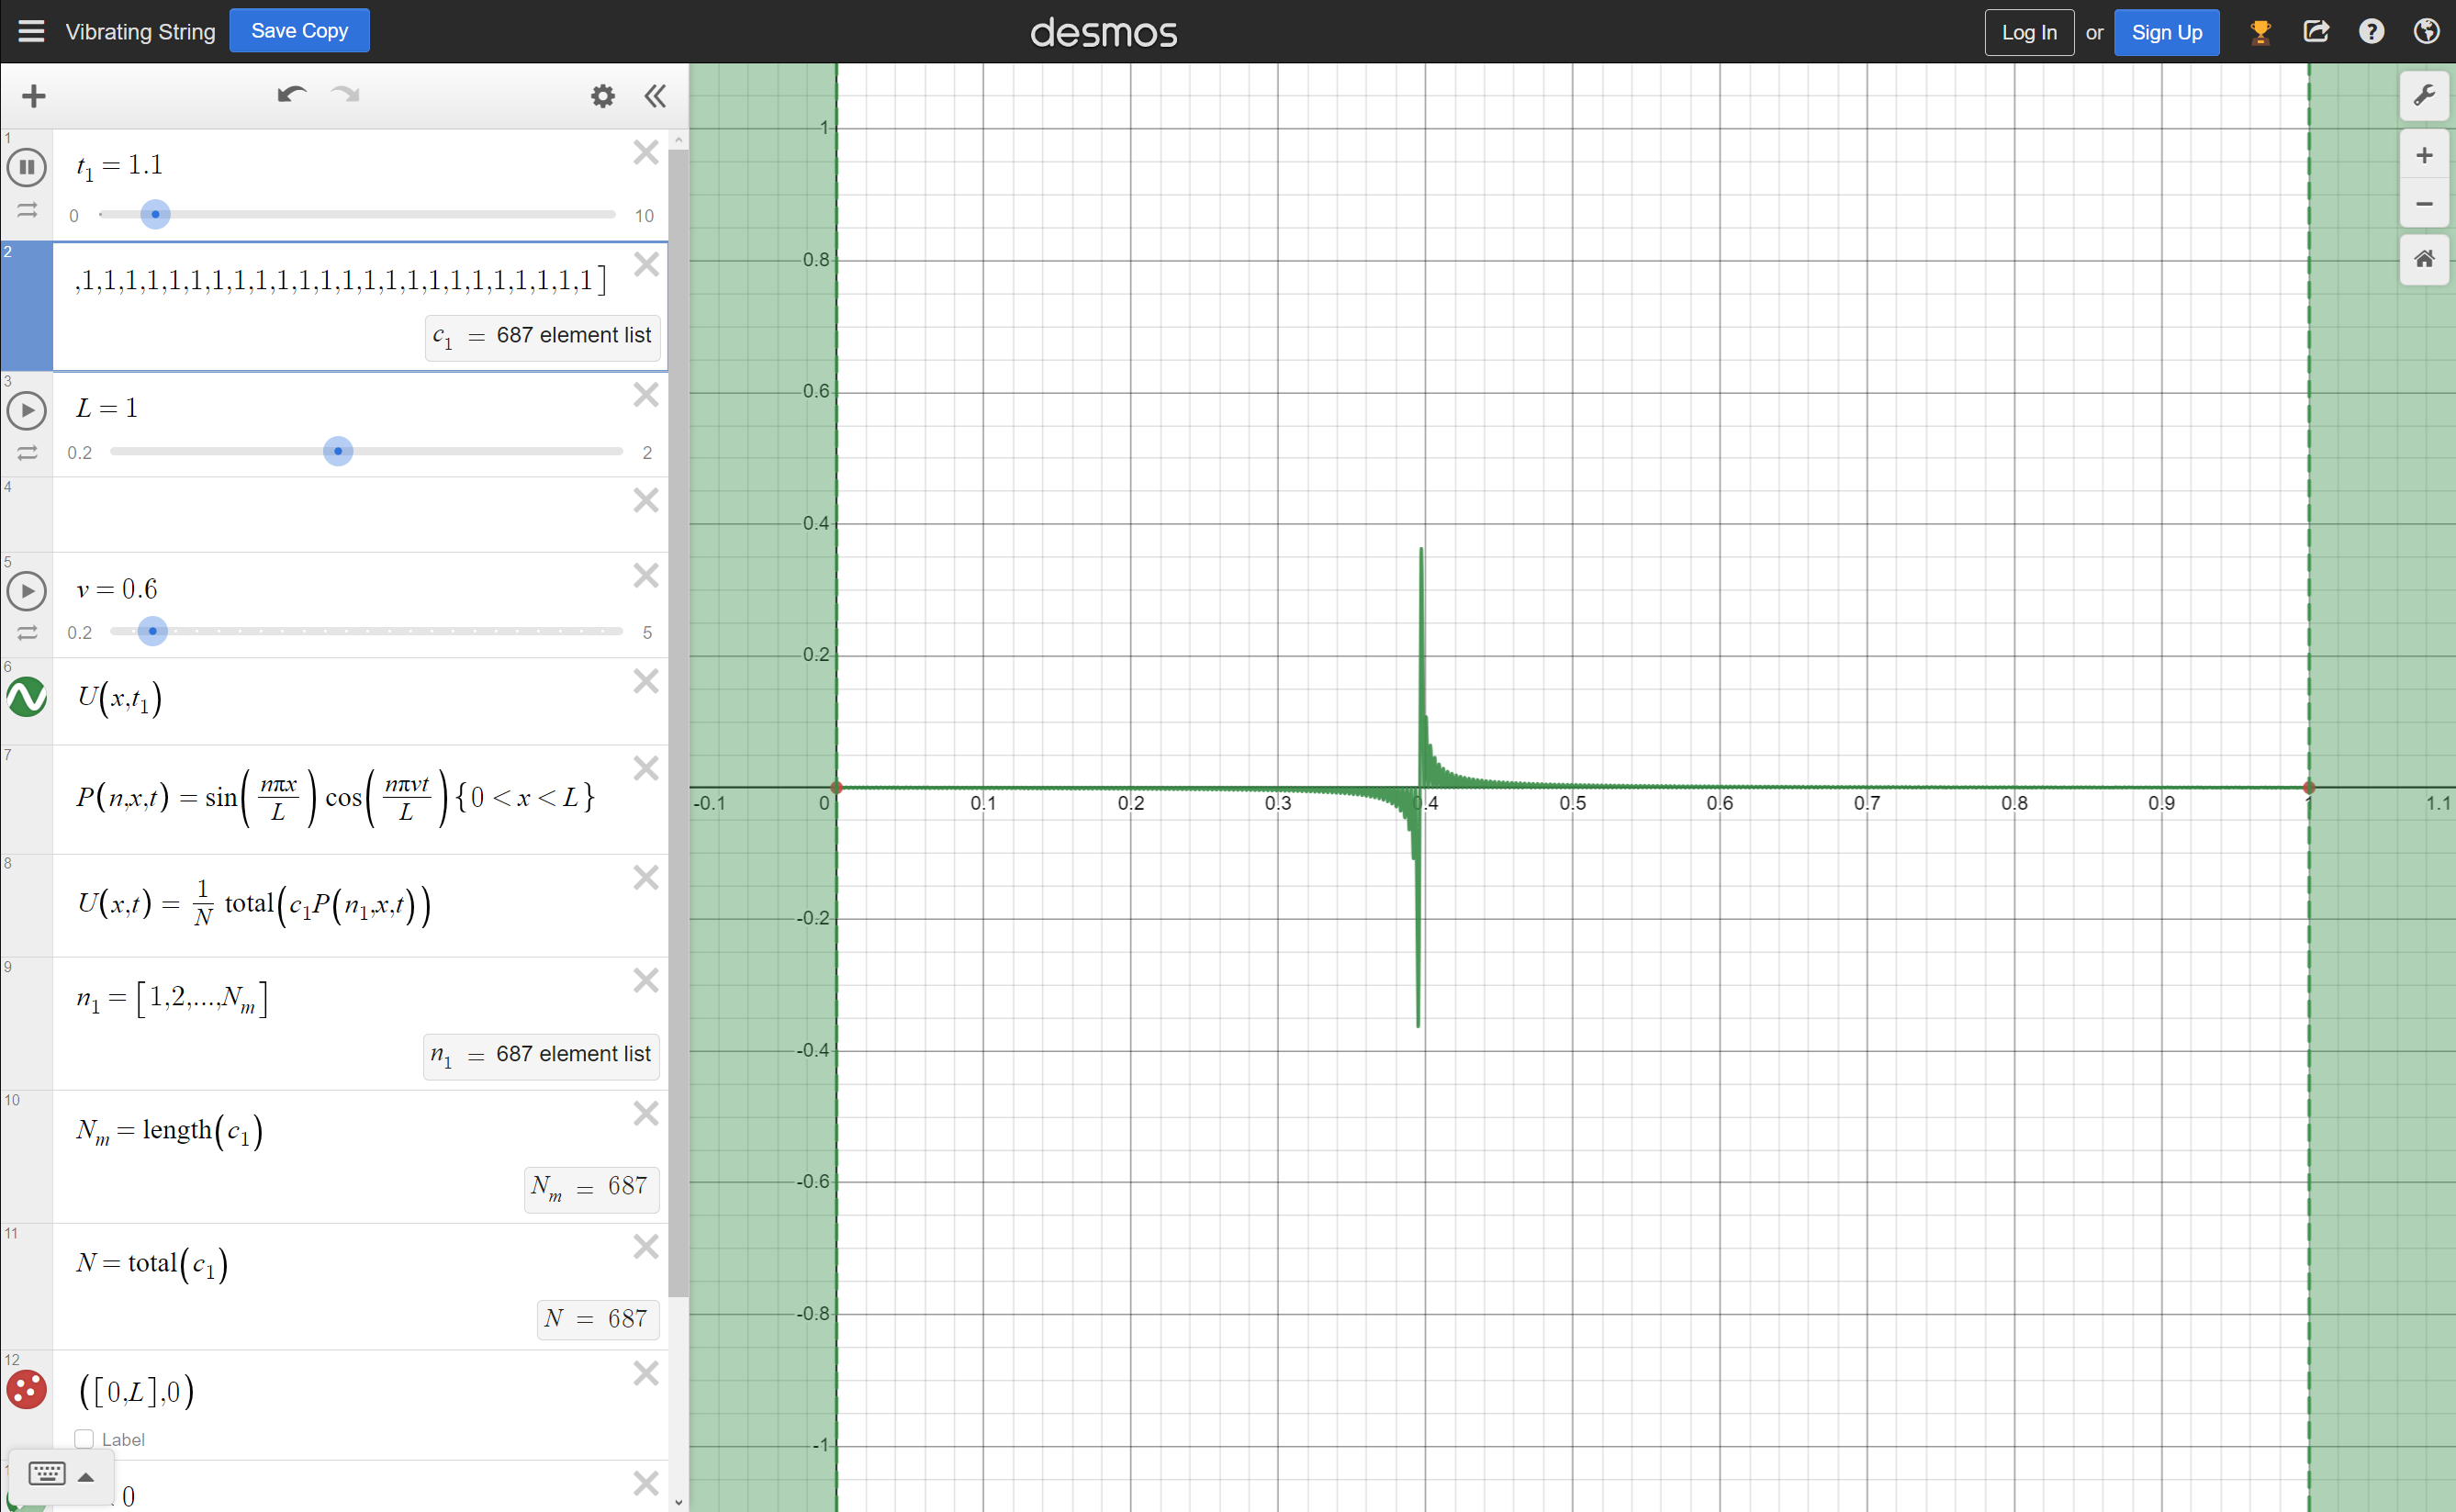
\includegraphics[scale=0.1]{Bilder/SamtaleTema1/Oppgave4b_2_prosjekt1.png}
    \caption{Figuren er hentet fra prosjekt i TFE4172, der mange bølger som løser TISE er lagt sammen for å produsere en kompakt bølgepakke. Produsert i desmos.}
    \label{fig:prosjekt1_eksempel}
\end{figure}

Som indikert til tidligere, henger HUP sammen med bølgepakker. Når bølger blir lagt sammen gir det utsving i en del av rommet, men selvom det fortsatt er en bølge er det en dårlig definert posisjon. 

Når vi måler bølgelengde/bevegelsesmengde vil vi kun få størrelsen fra en bølgene i bølgepakken, som da relativt til resten av bølgen er en viss usikkerhet ($\Delta p$). 

For mindre $\Delta x$ (mer nøyaktig posisjon) kreves flere bølger, men dette fører til støre $\Delta p$ (usikkert moment).

\subsection{Dobbelspalte eksperimentet}
\label{sec:tema1_9}
Isac Newton påstod at lys kun var bestående av partikler, men Thomas Young introduserte dobbelspalte ekperimentet. Eksperimentet gikk ut på å produsere en lyskilde, sende den gjennom to smale spalter som stod en avstand $d$ fra hverandre, og videre på en vegg bak (NB! viktig at disse avstandene er store relativ til spalteavstanden). For så å se om det dannet seg et mønster. I Youngs tilfelle så gjorde det det, og han var den første til å vise fenomenet inerferens. Det ga opphav til teorien om at lys hadde både partikkel egenskaper og bølge egenskaper.

Youngs eksperiment ble gjort i 1804, over hundre år før kvantemekanikken ble postulert, likevel er dobbelspalte eksperimentet essensielt til å vise at kvantepartikler innehar bølge egenskaper. Vi kan starte med å se på 3 eksempler, som bygger intuisjon for eksperimentet. Et med maskingevær kuler, vannbølger og sist lys.

\begin{figure}[!htb]
    \centering
    \includegraphics{Bilder/SamtaleTema1/maskingevær.png}
    \caption{Maskingevær som skytes mot to spalter.}
    \label{fig:Maskingevær}
\end{figure}

\begin{figure}[!htb]
    \centering
    \includegraphics{Bilder/SamtaleTema1/vannbølger.png}
    \caption{Plane Vannbølger som beveger seg mot to spalter.}
    \label{fig:vannbølger}
\end{figure}

\begin{figure}
    \centering
    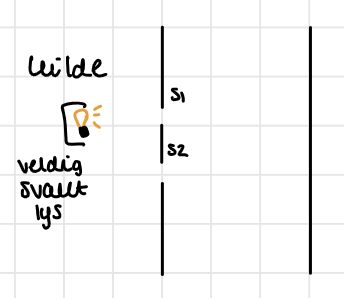
\includegraphics{Bilder/SamtaleTema1/lyskilde.png}
    \caption{Lyskilde som beveger seg mot to spalter, kan være en kontinuerlig lyskide eller eksitere atom slik at de sender ut fotoner (isåfall må man ha en film som tar imot denne energien, og det må være mørkt i rommet).}
    \label{fig:enter-label}
\end{figure}

\autoref{fig:resultaterDobbel} viser resultater fra dobbelspalte eksperimentet for de tre introduserte tilfellene. Vi ser at for maskingeværet vil det være tilfeldig spredning. for vannbølgen er resultatet som forventet, det oppstår destruktiv og konstruktiv interferens nå bølgen går gjennom. Så kommer vi til lyset, der et og et foton er ''skutt'' mot spaltene. Vi ser at det danner seg et interferens mønster, så lys har bølge egenskaper.

\begin{figure}[!htb]
    \centering
    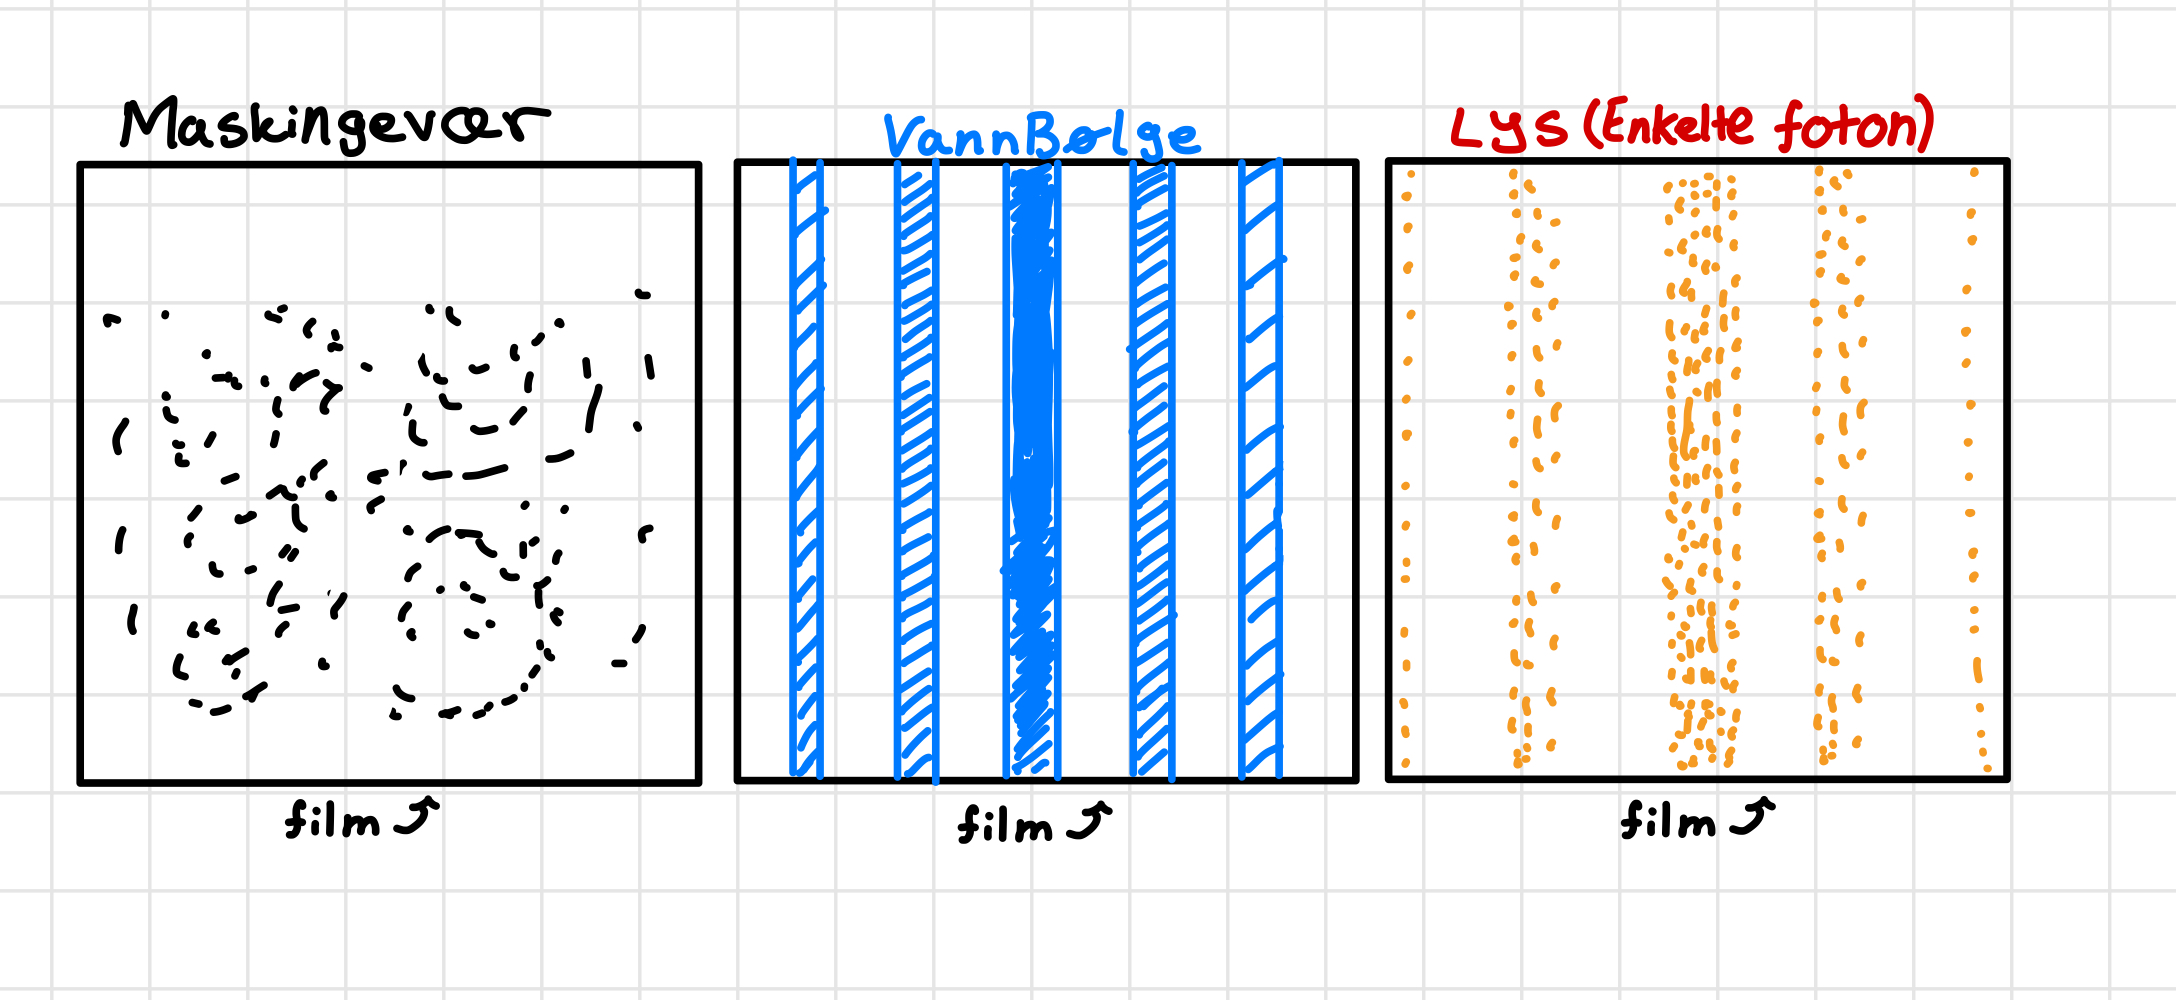
\includegraphics[scale=0.22]{Bilder/SamtaleTema1/ResultaterDobbelspalte.jpeg}
    \caption{Resultater fra dobbelspalte eksperimentet}
    \label{fig:resultaterDobbel}
\end{figure}

Vi kan si at interferens mønsteret som dannes er proporsjonal med $sinc$ funksjonen

\begin{equation}
    \label{eq:intensity}
    I(\theta) \thicksim I_0 (sinc(\beta))^2
\end{equation}

Nå er vel spørsmålet om kvantepartikler (elektron osv.) oppfører seg som bølger også? Det er litt komplisert, men vi prøver å forklare. La oss si at vi fører det samme eksperimentet vi hadde for lys. Når partikkelen skytes ut vil den inneha flere posisjoner samtidig i.e. den følger bølgefunksjonen og oppfører seg som en bølge, fra den treffer filmen og en ''måling'' blir tatt og vi avslører posisjonen som partikkelen har ''valgt''.

Nå kommer det som kanskje er litt vanskelig å skjønne, Hvis vi legger til en observator ved spaltene for å måle hvilken av de to spaltene partikkelen går gjennom, men da ser plutselig mønsteret på filmen mer ut som maskingevær fordelingen (!?) hvorfor det? Når vi tar en måling av partikkelen for å bestemme hvilken spalte den går gjennom, så må bølgefunksjonen kollapse, dette gjør at partikkeln må ''bestemme'' seg fr en posisjon og bevegelsesmengde. Det tar noen øyeblikk fra målingen er gjort til bølgefunksjonen gjenoppstår, og vi mister hele interferens mønsteret som egentlig skulle oppstått.

\begin{definition}
    \textbf{Bølge - partikkel dualiten: }om lys kan oppføre seg som partikler og bølger, kan partikler/materie oppføre seg som bølger.
\end{definition}

\section{Tema 2: Kvantebrønner}
\label{tema2}

\begin{table}[!htb]
    \centering
    \caption{Samtale punkter for tema 2}
    \begin{tabular}{|c|c|c|r|}
      \hline
      1 & Bundne og spredende tilstander &  \autoref{sec:tema2_1} & \cellcolor{blue}\quad\quad \\
      \hline 
      2 & Uendelig dyp kvantebrønn i 1D & \autoref{sec:tema2_2} & \cellcolor{green} \\
      \hline
      3 & Målepostulatet & \autoref{sec:tema2_3} & \cellcolor{green} \\
      \hline
      4 & Endelig kvantebrønn & \autoref{sec:tema2_4} & \cellcolor{blue} \\
      \hline 
      5 & Tunnellering & \autoref{sec:tema2_5} & \cellcolor{green} \\
      \hline
      6 & Pertubasjonsteori & \autoref{sec:tema2_6} & \cellcolor{green} \\ 
      \hline
    \end{tabular}
    \label{tab:samtalePunkt_tema1}
\end{table}

\subsection{Bundne og spredende tilstander}
\label{sec:tema2_1}
Bunnede og spredde tilstander er greit å ha en intuisjon om, kvantemekanikken er i hovedsak veldig lik den klassiske mekanikken, men med noen små avvik som vi skal gå inn på senere i \autoref{tema2}.

Enkelt forklart er bundet tilstander de tilstandene som binder et objekt. Se for deg du er i en berg og dalbane, bestående av en loop, start er bunnen av loopen, og det er også slutten. Si man kommer opp kvarte sirkelen. Bremsene slutter å funke og man sklir nedover igjen til start, i et system med energibevaring vil man ende like høy oppe på andre siden av loopen. Du er nå i en bundet tilstant, der den klassiske vendepunktet er punktet der du ikke har noe kinetiske energi, kun potensiell energi. \autoref{fig:bundet} er ikke berg og dalbane eksempelet, men med en generisk vogn.

\begin{figure}[!htb]
    \centering
    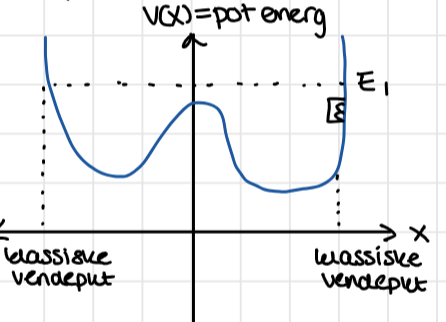
\includegraphics[scale=1]{Bilder/SamtaleTema2/Bundet og spredde/bundneTilstander.png}
    \caption{Systemet viser en vogn som er i en bundet tilstand}
    \label{fig:bundet}
\end{figure}

Vi kan spille videre på berg og dalbane eksempelet, se for deg en annen bane nå, der man kommer på flatmark i høy hastighet, foran deg er det en høyde. Den kinetiske energien til systemet gjør at man fyker rett over. Dette er et eksempel på en spredt tilstand, dersom du ikke kommer over vil du falle ned igjen på samme side, og forsvinne vekk fra høyden.

\begin{figure}[!htb]
    \centering
    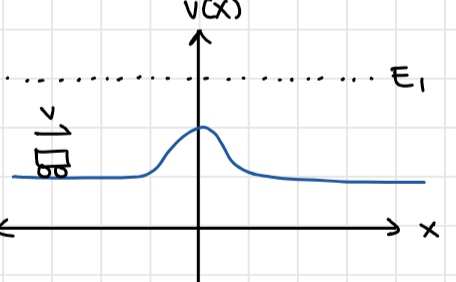
\includegraphics{Bilder/SamtaleTema2/Bundet og spredde/SpredteTilstander.png}
    \caption{Vogn på vei til en høyde, vognen er ikke låst til et område på x-aksen.}
    \label{fig:spredt}
\end{figure}
\newpage
\autoref{fig:kombinert} viser en figur der begge tilstandene oppstår, så avhengig av initial betingelsene kan en vogn ende opp med å bli bundet eller spred.

\begin{figure}[!htb]
    \centering
    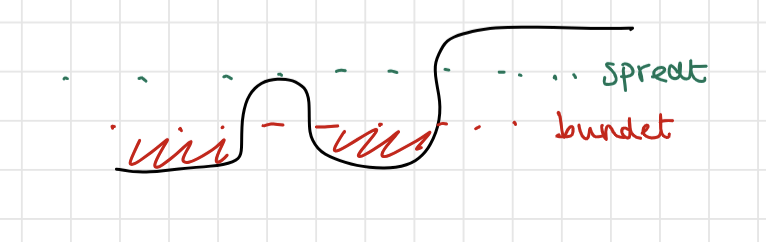
\includegraphics{Bilder/SamtaleTema2/Bundet og spredde/KombinerteTilstander.png}
    \caption{}
    \label{fig:kombinert}
\end{figure}

I kvantemekanikken oppfører en kvantepartikkel seg som det klassiske tilfellet, men ved de klassiske vendepunktene skjer det uventede. Vi starter med å se på SL for en kvantepartikkel i en potensiale.

\begin{equation}
    \label{eq:spredKvantte}
    \begin{split}
     E\psi(x)  &= -\frac{\hbar^2}{2m}\frac{\partial^2 \psi(x)}{\partial x} + V(x)\psi(x)\\
    \psi''(x) &= -\frac{2m(E-V(x))}{\hbar^2}\psi(x)\\
    \psi''(x) &= \alpha\psi(x)
    \end{split}
\end{equation}

vi kaller uttrykket foran $\psi(x)$ for $\alpha$. Vi på energien til partikkelen, dersom den er større enn potensialet $V(x)$ vil $\alpha < 0$ dette fører til trigonometriske løsninger, videre hvis energien $E < V(x)$ blir løsningen eksponentiell siden $\alpha > 0$.

I en uendelig kvantebrønn (se \autoref{sec:tema2_2}), kan man kun ha bundne tilstander, da det er ufysisk for en kvantepartikkel å være i et uendelig potensiale. I en endelig kvantebrønn er det ikke null sannsynlighet for at partikkelen eksisterer utenfor de klassiske grensene (se \autoref{sec:tema2_4}).

\renewcommand{\arraystretch}{1.5}% Vertically stretch tabular constructions
\noindent
\begin{tabularx}{\textwidth}{
    @{\hspace{1.5em}}% Space for left bullet
    >{\leavevmode\llap{\textbullet~}\raggedright}% Left bullet + formatting of column
    X% Left column specification
    @{\quad\hspace{1.5em}}% Space between columns + right bullet space
    >{\leavevmode\llap{\textbullet~}\raggedright\arraybackslash}% Right bullet + formatting of column
    X% Right column specification
    @{}% No column space on right
  }
  \toprule
  \multicolumn{1}{X}{\centering\bfseries Bundne Tilstander} &
    \multicolumn{1}{X}{\centering\bfseries Spredde Tilstander} \\
  \midrule
    Avgrenset i rom  & 
    Ikke avgrenset i rom  \\
    Normaliserbare ($\psi$ går mot 0 ved $\pm \infty$) & ikke normaliserbare ( bølgefunksjonen har ikke definert areal under grafen) \\
    Kvantiserte av randbetingelser (randbetingelsene begrenser energinivåene som er tilgjengelige for systemet, og disse energinivåene er kvantisert) & 
    Ikke kvantiserte (kontinuerlig spektrum, alle energinivåer lov) \\
    De antar bare diskrete bestemte verdier & - \\
  \bottomrule
\end{tabularx}

\begin{figure}[!htb]
    \centering
    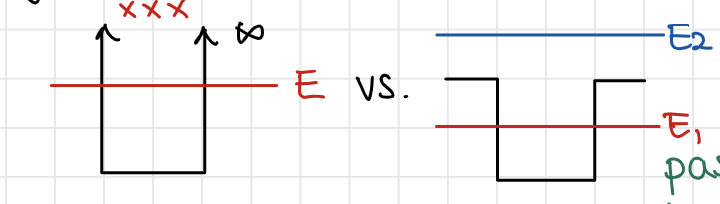
\includegraphics{Bilder/SamtaleTema2/Bundet og spredde/endeligvsuendelig.png}
    \caption{Røde kryssene over uendelig kvantebrønn indikerer at det ikke er mulig å ha energi utenfor brønnen, men dette er mulig for den endelige brønnen.}
    \label{fig:endeligVSuendelig}
\end{figure}

\newpage
\subsection{Uendelig dyp kvantebrønn i 1D}
\label{sec:tema2_2}
\subsubsection{Fri partikkel}
Før vi kan se på en uendeig dyp kvantebrønn, kan vi se på en fri partikkel. Partikkelen er ikke påvirket av et potensial, så all energien til partikkelen er ''bakt'' inn i bevegelsesmengden. I \autoref{eq:shrodinger_freeparticle} har vi allerrede sett uttrykket og seksjonen går litt inn på utledningen. Vi vil gjerne se på et plot som sammenligner energien og bølgetallet $k$, ved å forenkle ligning \ref{eq:shrodinger_freeparticle} får vi 

\begin{equation}
    \label{eq:free_part_simplified}
    \frac{\hbar^2}{2m} \frac{\partial^2 \psi(x)}{\partial x^2} + E\psi(x) = 0,
\end{equation}

Løsningen til ligning \ref{eq:free_part_simplified} er en funksjon som også er egentilstanden til både energi og bevegelsesmengde.

\begin{equation}
\label{eq:solPsi_freeparticle}
    \psi(x) = Ae^{ikx}
\end{equation}

Setter vi ligning \ref{eq:solPsi_freeparticle} inn i ligning \ref{eq:free_part_simplified} får vi

\begin{equation}
    \label{eq:freeLastEq}
    -\frac{\hbar^2k^2}{2m}\psi(x) + E\psi(x) = 0,
\end{equation}

Vi sitter igjen med at det kun er én ikke triviell løsning til ligning \ref{eq:freeLastEq}. \autoref{eq:Evalue_free} viser bevegelsesmengde energien.

\begin{empheq}[box=\tcbhighmath]{align}
    \label{eq:Evalue_free}
    E = \frac{\hbar^2k^2}{2m}
\end{empheq}

Vi ser nå at forholdet mellom energien og bølgetallet er kvadratisk. \autoref{fig:parabola} viser en parabel. Denne funksjonen er kontinuerlig, Energien i dette tilfellet er ikke kvantisert.

\begin{figure}[!htb]
    \centering
    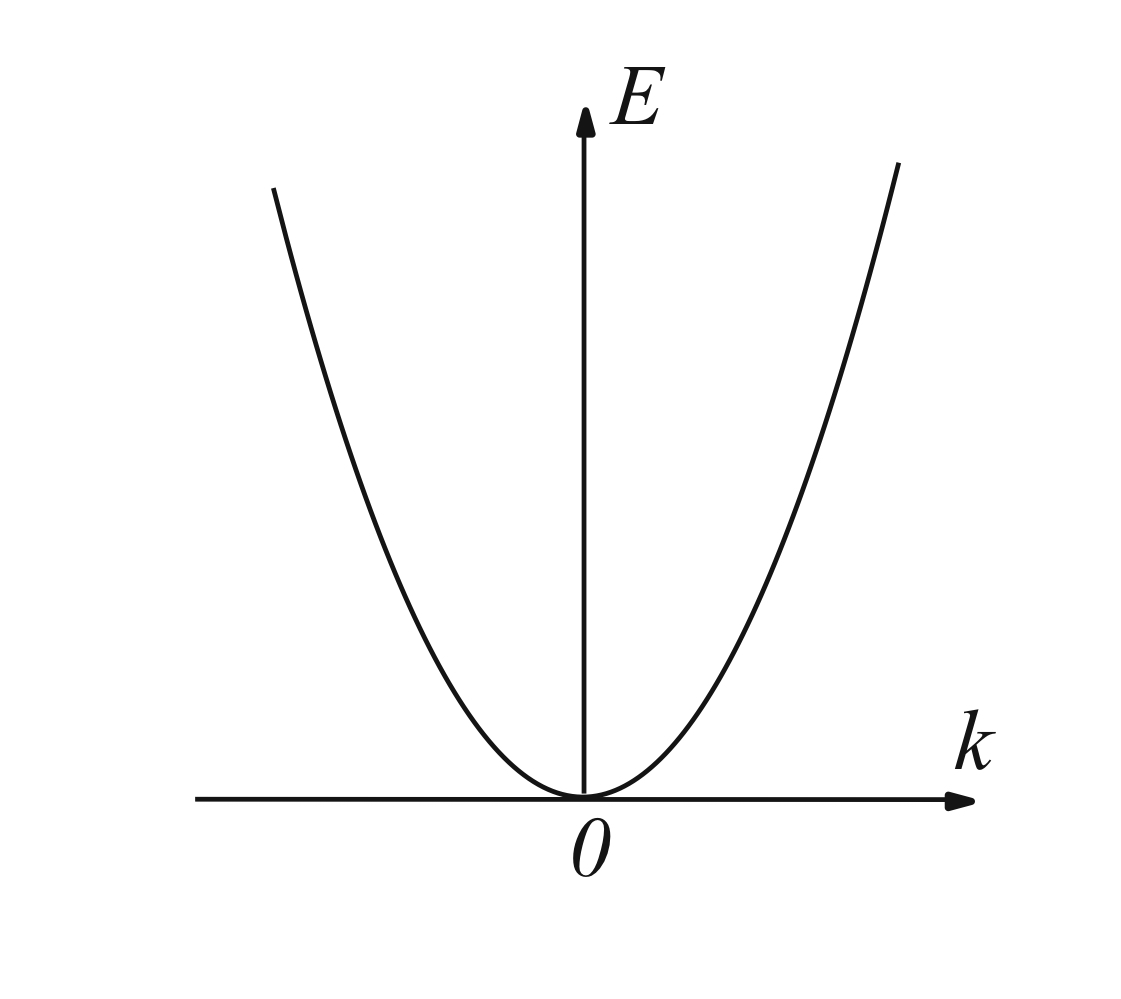
\includegraphics[scale=0.25]{Bilder/SamtaleTema2/FreeParticleEnergy.jpg}
    \caption{Energi - bevegelsesmengde forholdet for en fri partikkel}
    \label{fig:parabola}
\end{figure}

Intervallet partikkelen vil kunne bevege seg på er $[-L,L]$, der $L$ går mot $\infty$.

\subsubsection{Uendelig dyp kvantebrønn 1D}
Ved å begrense partikkelen og innføre grensebetingelser får vi en litt annen oppførsel. Vi sier at partikkelen kan bevege seg mellom $[0,a]$ der $a$ har en definert verdi. Potensialet til brønnen kan representeres som

\begin{equation}
\label{eq:potInfinite}
V(x) = \left\{
        \begin{array}{ll}
            -\infty & \quad x \leq 0 \\
            0 & \quad 0 \leq x \geq a \\
            \infty & \quad x \geq a
        \end{array}
    \right.
\end{equation}

Ved å ta i bruk funksjonen for spenningen fra ligning \ref{eq:potInfinite} kan vi skissere opp systemet, dette er visualisert i figur \ref{fig:1DInfWell}

\begin{figure}[!htb]
    \centering
    \includegraphics[scale=0.2]{Bilder/SamtaleTema2/1DUendeligBrønn.jpg}
    \caption{Potensiell energi for en 1D box.}
    \label{fig:1DInfWell}
\end{figure}

Konsekvensen av å sette potensialet lik $\infty$ utenfor den en dimensjonale boksen gjør at bølgefunksjonen $\psi(x)$ vil være null. Fordi en partikkel ikke kan inneha uendelig energi. Dette fører også til at vi får grensebetingelser på systemet vårt, representert med ligning \ref{eq:randBetingelser1D}

\begin{equation}
    \label{eq:randBetingelser1D}
    \psi(0) = \psi(a) = 0
\end{equation}

\autoref{eq:solPsi_freeparticle} er en løsning for dette systemet også, men det er gunstig å skrive det om til sinus og cosinus. 

\begin{equation}
    \psi(x) = Asin(kx) + Bcos(kx)
\end{equation}

løser vi med hensyn på randbetingelsene får vi at $B=0$ og $Asin(ka)=0$. Siden bølgefunksjonen ikke kan være null i hele rommet, må det bety at 

\begin{equation}
    ka = n\pi \implies k_n = n\frac{\pi}{a},
\end{equation}

Vi ser nå at i motsetning til fri partikkel, kan ikke bølgenummeret k være en kontinuerlig funksjon, altså energinivåene er kvantiserte. Energi uttrykket kan skrives som 

\begin{empheq}[box=\tcbhighmath]{align}
    \label{eq:1D-particleEnergy}
    E_n = \frac{\hbar^2 \pi^2 n^2}{2ma^2}
\end{empheq}

For å finne normaliseringskonstanten er det bare å sette inn i ligning \ref{eq:normalisering}, og framgangsmåten er relativt intuitiv.

\subsection{Målepostulatet}
\label{sec:tema2_3}
Målepostulatet i kvantemekanikken sier at når vi gjør en måling av en kvantepartikkel (f.eks posisjon eller spinn), får vi et bestemt resultat med en viss sannsynlighet. 

For at en løsning til SL skal kunne representere en partikkel må denne løsningen være ''normaliserbar''. Normalisering er bevart over tid dersom $\hat{H}$ er en Hermittisk operator. En Hermittisk operator er en operator som oppfyller ligning \ref{eq:hermit}

\begin{equation}
    \label{eq:hermit}
    \int \Psi_1^*\hat{H}\Psi_2 = \int \bigl(\hat{H}\Psi_1\bigl)^*\Psi_2
\end{equation}

Dette er også sant for $\Psi_2^*\Psi_1$ og $\Psi_1^*\Psi_1$. Hermittiske operatorer har alltid reelle egenverdier

\begin{equation}
    \hat{H}\psi = E\psi
\end{equation}
Her er $E$ en egenverdi og $\psi$ er en egenfunksjon. Så alle operatorer som produserer reelle egenverdier er Hermittiske.

Hermittiske operatorer har et komplett sett av ortonormale egenfunksjoner. Funksjonen står vinkelrett på hverandre dersom det indreproduktet er lik null. For bølgefunksjonen får vi

\begin{equation}
\label{eq:hemittisk}
\int \Psi_m^*\Psi_n = \delta_{mn} \left\{
        \begin{array}{ll}
            0 & \quad m \neq n \\
            1 & \quad m = n 
        \end{array}
    \right.
\end{equation}

Fra det komplette settet kan vi representere en hver relevant bølgefunksjon ved superposisjon

\begin{equation}
    \label{eq:superpos}
    \psi(x) = \alpha_1\psi_1{x} + \alpha_2\psi_2{x} + \alpha_3\psi_3{x} + ...
\end{equation}

$\alpha_i$ er i dette tilfellet en sannsynlighetsvekt, så dersom vi skulle målt en av bølgene må en av disse velges ved kollapsen av bølgefunksjonen. Dersom vi har en vilkårlig Hermittisk operator vi kaller $\hat{Q}$, og anvender denne på $\psi$ vil vi \textbf{kun} måle en av egenverdiene. og sannsynligheten for å måle $q_i$ er

\begin{equation}
    p_i = |\alpha_i|^2 = \int \psi_i^*\psi dx
\end{equation}

Etter utfallet av $q_i$ er målt, blir tilstanden til systemet $\psi(x)=\psi_i(x)$. Vi sier med det at bølgefunksjonen har kollapset. Dersom det blir gjort en måling rett etter, vil resultatet være det samme. Men etter tid vil bølgefunksjonen inneha et likt ''uordnet'' system.

\subsection{Endelig kvantebrønn}
\label{sec:tema2_4}
\autoref{fig:finiteSquare} viser en endelig kvantebrønn, hvis en partikkel har total energi som er større enn $V_0$ vil vi ha en spredende tilstand, vi er ikke interessert i disse i dette kapitellet. Vi kan dele systemet inn i tre soner, \rom{1} er alt til venstre for $-\frac{a}{2}$ og \rom{3} er alt til høyre for $\frac{a}{2}$. Region \rom{2} er området i mellom \rom{1} og \rom{3}.

\begin{figure}[!htb]
    \centering 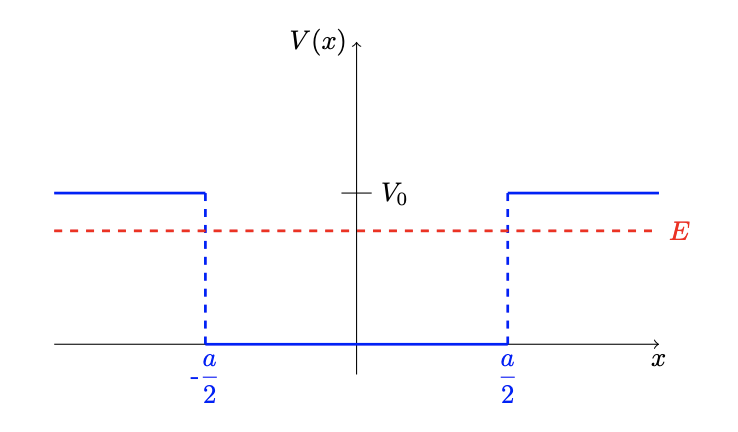
\includegraphics[scale=1]{Bilder/SamtaleTema2/endeligKvanteBrønn/FiniteSquare.png}
    \put(-300,80){\rom{1}}
    \put(-190,80){\rom{2}}
    \put(-80,80){\rom{3}}
    \caption{Endelig kvantebrønn, fortsatt 1D (partikkelen lever på x-aksen)}
    \label{fig:finiteSquare}
\end{figure}

sone \rom{1} og \rom{3} er klassiske forbudte områder, men en kvantepartikkel kan finne på å ende opp der. I region \rom{2} er 
$\alpha < 0$ (samme $\alpha$ fra ligning \ref{eq:spredKvantte}, vi får trigonometriske løsninger. Region \rom{1} og \rom{3} vil ha $\alpha > 0$ som gir oss eksponentielle løsninger.

\begin{figure}[!htb]
    \centering
    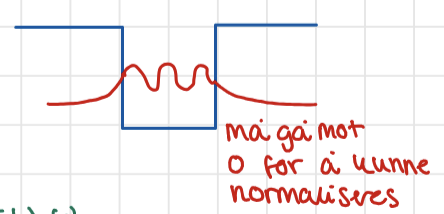
\includegraphics[scale=1]{Bilder/SamtaleTema2/endeligKvanteBrønn/nrmali.png}
    \caption{Viser oss at sannsynligheten for å finne en bølge utenfor det klassiske forbudte området er større enn null}
    \label{fig:normalComment}
\end{figure}

Viktige kriterier for løsningen av problemmet endelig kvantebrønn er veldig lik kriteriene for den uendelige kvantebrønnen er randbetingelsene. Men nå har vi også

\begin{equation*}
    \begin{split}
        \psi_{\rom{1}}(-\frac{a}{2}) &= \psi_{\rom{2}}(-\frac{a}{2}) \\
        \psi_{\rom{2}}(\frac{a}{2}) &= \psi_{\rom{3}}(\frac{a}{2}) \\
        \frac{\partial}{\partial x}\psi_{\rom{1}}(-\frac{a}{2}) &= \frac{\partial}{\partial x}\psi_{\rom{2}}(-\frac{a}{2}) \\
        \frac{\partial}{\partial x}\psi_{\rom{2}}(\frac{a}{2}) &= \frac{\partial}{\partial x}\psi_{\rom{3}}(\frac{a}{2}) 
    \end{split}
\end{equation*}

Vi definerer nå variabelen k som 

\begin{equation}
\label{eq:k_endelig}
    k^2 = \frac{2m}{\hbar^2}(V_0-|E|) > 0
\end{equation}

Uttrykket $V_0-|E|$ sier oss noe om ''avstanden'' fra potensial til energi. Innenfor region \rom{2} er den større enn null.

Sette vi inn det vi har til nå i SL får vi at $\psi'' = -k^2\psi$, dette gir sin/cos løsninger, men siden vi har kun har symmetriske løsninger kan vi si at

\begin{equation}
    \psi(x) = ... cos(kx) \quad ; \quad -\frac{a}{2} < x < \frac{a}{2}
\end{equation}

I dette tilfellet dropper vi normaliseringskonstanten. Løsningen for region \rom{3} blir lik som for region \rom{1}. Ved utledning finner vi

\begin{equation}
\label{eq:3}
\begin{split}
    \psi''(x) &= -\frac{2m}{\hbar^2}E\psi(x) \\
    \psi''(x) &= \frac{2m|E|}{\hbar^2}\psi(x) \\
    \psi''(x) &= \kappa^2\psi(x)
\end{split}
\end{equation}

Løser ligningen vi sitter igjen med fra \ref{eq:3}, får vi for $\psi(x)$ to løsninger

\begin{equation}
    \label{eq:sol1_sol3}
    \psi(x) = Ae^{\pm kx}
\end{equation}

\autoref{eq:sol1_sol3} viser oss at ved $x<-\frac{a}{2}$ får vi en positiv eksponent, og for $x>\frac{a}{2}$ får vi en negativ en, så når begge sider går mot uendelig går bølgefunksjonen mot null.

For å gjøre neste delen litt enklere gjør vi om bredden på brønnen til å gå fra $-a$ til $a$, dette gjør noen av uttrykkene litt enklere å jobbe med. 

Vi har nå to bølgetall, $\kappa$ og $k$. De hører til forskjellige regioner. Man kan tolke det som lysbølge som beveger seg  vakuum sammenlignet med i vann. Når den beveger seg i vakuum har bølgen et spesefikt bølgetall, mens når den beveger seg i vann har den et annet. Dette kan sammenlignes med potensialet $V(x)$, når bølgen er utenfor det klassiske området vil potensialet være anerledes, og dermd gir det et annet bølgetall sammenlignet med det som oppstå i brønnen.

\begin{equation}
\label{eq:kappashit}
    \begin{split}
        \kappa^2 + k^2 &= \frac{2mV_0}{\hbar^2} \\
        \kappa^2a^2 + k^2a^2 &= \frac{2mV_0a^2}{\hbar^2}, \quad \zeta = \kappa a,\, \eta = ka \\
        \zeta^2 + \eta^2 &= Z_0^2
    \end{split}
\end{equation}

\autoref{eq:kappashit} viser en ligning som forteller oss om forholdet mellom bølgetallene, på høyre siden sitter vi igjen med et uttrykk som forteller oss om den endelige kvantebrønnen vi ser på. Siden $\zeta> 0$ og $\eta>0$, får vi en kvart sirkel i $\zeta$- og $\eta$-planet.

$\psi$ er kontinuerlig i $x=a$ det gir oss
\begin{equation}
\label{eq:1}
    cos(ka)=Ae^{-\kappa a}
\end{equation}
og $\psi'$ er også kontinuerlig i $x = a$ som gir
\begin{equation}
\label{eq:2}
    ksin(ka) = \kappa Ae^{-\kappa a}
\end{equation}

Både ligning \ref{eq:1} og \ref{eq:2} representerer grensebetingelsene i overgangen mellom region \rom{2} og \rom{3}. Dersom vi deler ligning \ref{eq:1} på ligning \ref{eq:2} får vi

\begin{equation}
\label{eq:even}
    \frac{\rom{2}}{\rom{1}} \, : \,
    ktan(ka) = \kappa \implies \zeta = \eta tan(\eta),
\end{equation}

for den like løsningen, og for den odde løsningen får vi

\begin{equation}
    \label{eq:odd}
    \zeta = -\eta cot(\eta)
\end{equation}

\autoref{fig:losningEndeligGrafisk} 

\begin{figure}[!htb]
    \centering
    \subfloat[\centering Like løsninger fra ligning \ref{eq:even}]{{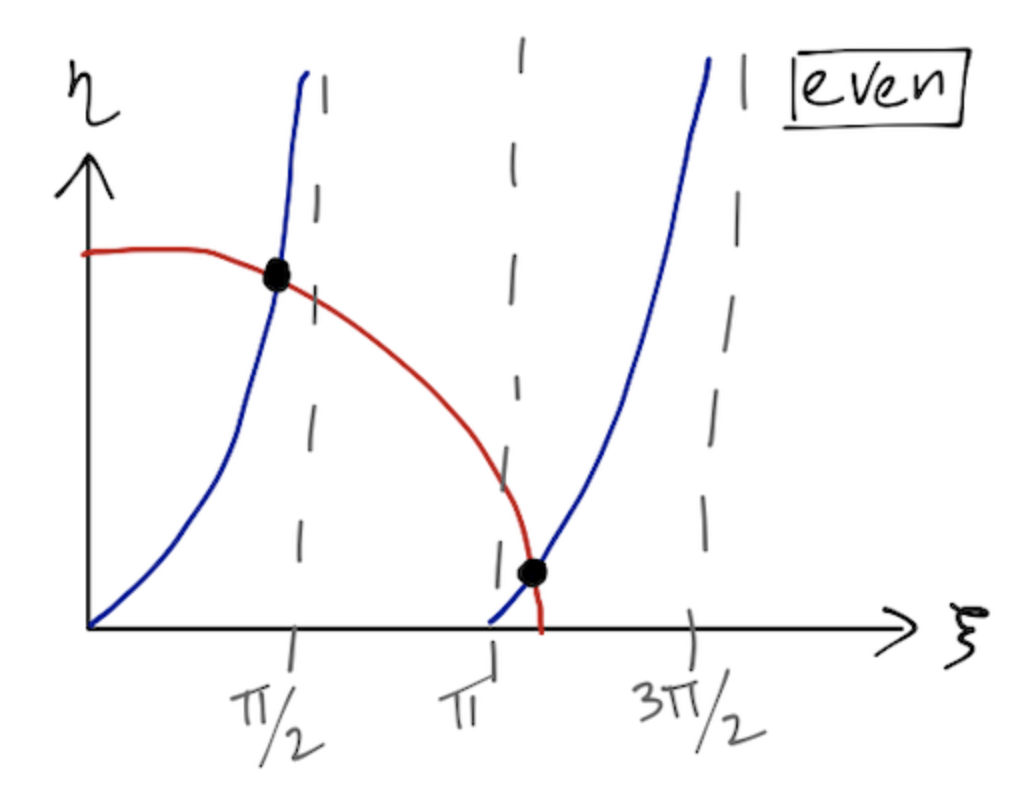
\includegraphics[width=7cm]{Bilder/SamtaleTema2/endeligKvanteBrønn/evenSol.png} }}%
    \qquad
    \subfloat[\centering Odde løsninger fra ligning \ref{eq:odd}]{{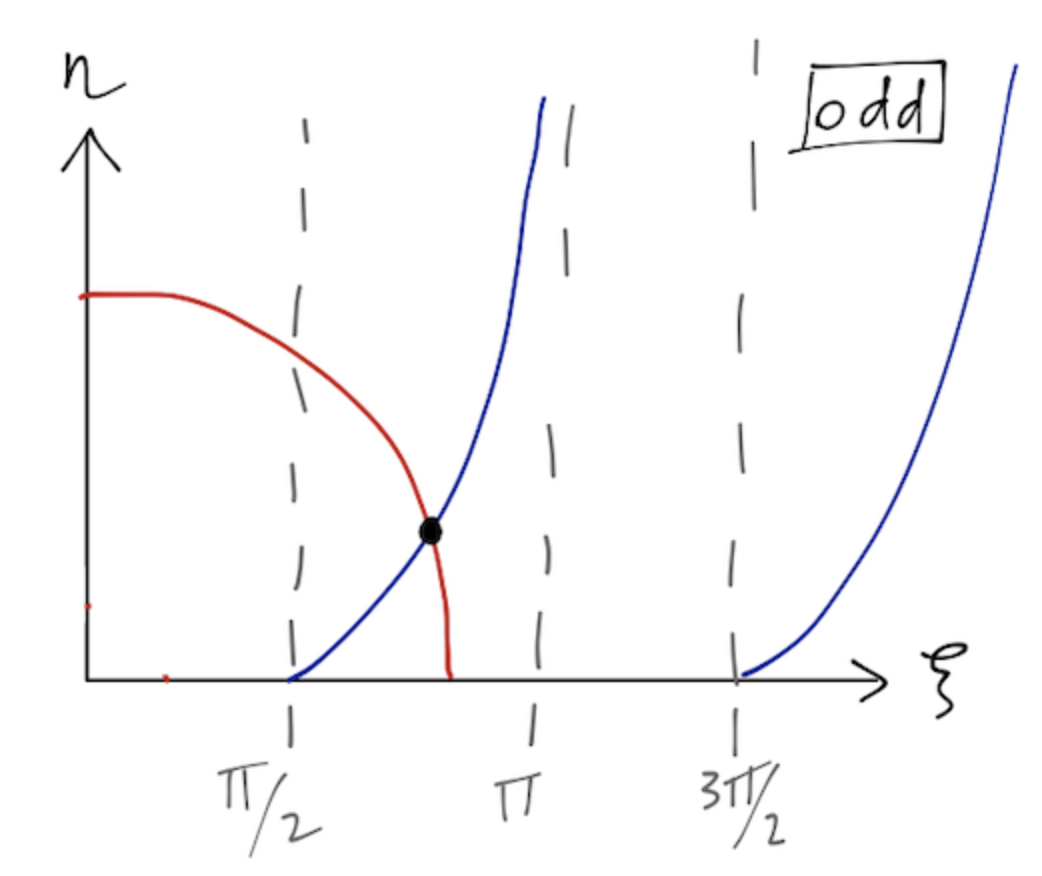
\includegraphics[width=7cm]{Bilder/SamtaleTema2/endeligKvanteBrønn/oddSol.png} }}%
    \caption{2 Figures side by side}%
    \label{fig:losningEndeligGrafisk}%
\end{figure}

NB! aksene her er ikke riktig, $\zeta$ skal være på y-aksen og $\eta$ skal på x-aksen.

Selvom $Z_0$ (radiusen til den røde sirkelen) er liten i.e. brønnen er veldig lite dyp, vil det alltid være plass til minst en bølgefunksjon. 

Tilegg: Potensialet  $V_0$ er det som bestemmer ''dybden'' på den endelige kvantebrønnen. det er derimot energien $E$ som bestemmer hvor ''høyt'' oppe partikkelen kan befinne seg.

\subsection{Tunnellering}
\label{sec:tema2_5}
Tunnellering er et kvantemekaniske fenomen der en partikkel klarer å bevege seg gjennom en barriere av potensiell energi som har en høyere energi enn partikkelens kinetiske energi. Mer som dette i \autoref{tema3}.

\subsection{Pertubasjonsteori}
\label{sec:tema2_6}
Pertubasjonsteori er en systematisk metode for å finne tilnærmede løsninger til perturberte kvantemekaniske system. Kravet for å anvende teorien er at perturabsjonen er ''liten'' og løsninger for det uperturberte systemet er kjent. Det vil si at dersom vi legger en perturbasjone i en uendelig kvantebrønn, kjenner vi allerede løsningen for det uperturberte systemet. Vi kan derfor bruke det som utgangspunkt til å finne løsningen til det perturberte sysemet. 

Det vi ønsker å finne med perturbasjonteori er en Hamiltonian som for det perturberte systemet. En kan se på en perturbasjon som en forstyrrelse i form av et potensial som blir lagt til i systemet. Vi definerer løsningen til det uperturberet systemet som 

\begin{equation}
    \label{eq:solUpert}
    \hat{H}^{(0)}\psi_n^{(0)} = E_n^{(0)}\psi_n^{(0)},
\end{equation}

For det perturberte systemet blir dette 

\begin{equation}
    \label{eq:hamPert}
    \hat{H} = \hat{H}^{(0)} + \hat{u}_{pert}
\end{equation}

Pertubasjonsteori gir oss den totale energien og bølgefunksjonen som en sum av korreksjonsedd. Dersom antall ledd går mot uendelig vil løsningen være riktig, men dette gjelder kun for ikke analytiske systemer. lignende taylor rekker vil det første leddet bære med vekt og leddene sine vekter vil anta ettersom ledd indexen øker.

\begin{equation}
    \label{eq:pertEnergi}
    E_n = E_n^{(0)} + E_n^{(1)} + E_n^{(2)} + ... + E_n^{(m)}
\end{equation}

\begin{equation}
    \label{eq:pertWave}
    \psi_n = \psi_n^{(0)} + \psi_n^{(1)}  + \psi_n^{(2)}+ ... + \psi_n^{(m)} 
\end{equation}

Første ordens korreksjons ledd for $E_n$

\begin{equation}
    E_n^{(1)} = \bra{n^{(0)}} \hat{u}_{pert} \ket{n^{(0)}}
    =
    \int_{-\infty}^{\infty} \psi_n^{(0)*}u_{pert}\psi_n^{(0)}dx
\end{equation}

Den perturberte løsningen inneholder litt høyere energi, dette er fordi tilførselen av et potensial i den endelig kvantebrønnen gjør at det innføres mer krumming i bølgefunksjonen, og energi er proporsjonalt med krumningen til bølgefunksjonen. 

\begin{figure}[!htb]
    \centering
    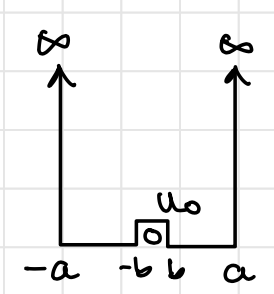
\includegraphics{Bilder/SamtaleTema2/Pertubasjonsteori/pert.png}
    \caption{Endelig kvantebrønn med tilførsel av en perturbasjon lokalisert i midten av brønnen.}
    \label{fig:figPert}
\end{figure}

\newpage

\section{Tema 3: Atom og bindinger}
\label{tema3}

\begin{table}[!htb]
    \centering
    \caption{Samtale punkter tema 3}
    \begin{tabular}{|c|c|c|r|}
      \hline
      1 & Kvantebrønn i 3D (partikkel i boks) &  \autoref{sec:tema3_1} & \cellcolor{blue}\quad\quad \\
      \hline 
      2 & Degenerasjon & \autoref{sec:tema3_2} & \cellcolor{blue} \\
      \hline
      3 & Hydrogenatomet & \autoref{sec:tema3_3} & \cellcolor{blue} \\
      \hline
      4 & Det periodiske systemet og Elektronkonfigurasjon & \autoref{sec:tema3_4} & \cellcolor{blue} \\
      \hline 
      5 & Bindinger i faste stoffer & \autoref{sec:tema3_6} & \cellcolor{green} \\ 
      \hline
      6 & Dobbel kvantebrønn & \autoref{sec:tema3_7} & \cellcolor{blue} \\
      \hline
      7 & Det interatomære potensiale & \autoref{sec:tema3_8} & \cellcolor{blue} \\
      \hline
    \end{tabular}
    \label{tab:samtalePunkt_tema1}
\end{table}

\subsection{Kvantebrønn i 3D (partikkel i boks)}
\label{sec:tema3_1}
Vi beveger oss fra å jobbe i 1D til 3D, men løsningen på partikkel i boks har lignende løsning som partikkel i 1D brønn. \autoref{eq:1D-Sol} viser løsningen på problemet i 1D.

\begin{equation}
\label{eq:1D-Sol}
    \bigg[
    \psi_n(x) = \sqrt{\frac{1}{a}}sin\bigg(\frac{n\pi x}{L}\bigg),
    \;E_n = \frac{n^2\pi^2\hbar^2}{2ma^2}
    \bigg]
\end{equation}

I 3D legger vi til litt komplekst, vi antar nå vi har en kube, så alle veggene er $a$ lange i $x$-, $y$- og $z$-retning. Dette gir \ref{eq:3D-sol}

\begin{equation}
    \label{eq:3D-sol}
    \psi(x,y,z) = \sqrt{\frac{2^3}{a^3}}
    sin\bigg(\frac{n_x\pi x}{a}\bigg)
    sin\bigg(\frac{n_y\pi y}{a}\bigg)
    sin\bigg(\frac{n_z\pi z}{a}\bigg)
\end{equation}

og energien kommer ut på formen 

\begin{equation}
    \label{eq:3D-energi}
    E_{n_xn_yn_z} = \frac{\pi^2\hbar^2}{2ma^2}
    \bigg(
    n_x^2+n_y^2+n_z^2
    \bigg)
\end{equation}

I ligning \ref{eq:3D-energi} står $n_i$ for kvantetall, altså kun positive heltall fra $1$ og oppover. Ulike kombinasjoner kan produsere sammen energi, men de ulike kombinasjonene produserer samme energi kan de ikke ha lik bølgefunksjon $\psi(x,y,z)$, dette ser vi siden $n_i$ inngår i sine respektive sinus funksjoner.

\subsection{Degenerasjon}
\label{sec:tema3_2}
\autoref{fig:degen_energi} viser oversikt over energitilstander med tilhørende kvantetall. Det er synlig at f.eks første energi nivå har vi at alle kvantetallene er $1$. Dette er ikke en degenerert tilstand, da det kun er en bølgefunksjon som korresponderer med energi nivået. En degenerert tilstand er definert som en tilstand der et system kan ha lik energi i flere konfigurasjoner av kvantetall, men ulike bølgefunksjoner. 

\begin{figure}[!htb]
    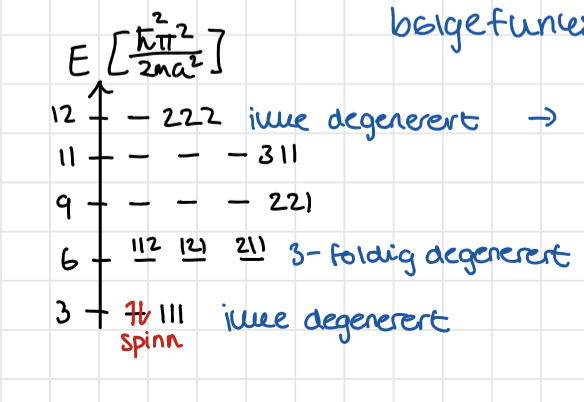
\includegraphics[width=0.9\textwidth]{Bilder/SamtaleTema3/3D partikkel i boks/degenererteTilstander.png}
    \caption{Oversikt over energitilstander og degenererte tilstander}
    \label{fig:degen_energi}
\end{figure}

Lengden på sidene av den 3D boksen er viktig, det er også symmetri når det kommer til degenerasjon. Om alle sidene hadde vært forskjellige hadde \textbf{alle} energinivåene vært separert. \color{red} Degernasjon er et resultat av symmetri i systemet. \color{black}

Som man ser fra figur \ref{fig:degen_energi}, ligger det to piler på det laveste energi nivået, grunntilstanden om man vil. Disse pilene representerer spinn. Elektroner har en kvantemekanisk egenskap som gjør at de spinner, det finnes kun to spinn konfigurasjoner, spinn opp og spinn ned. Dette fører oss til et resultat som Wolfgang Pauli postulerte i 1925, det fikk navnet Paulis eksklusjonsprinsipp.

\begin{definition}
    \textbf{Pauls ekslusjonsprinsipp}: To eller flere fermioner kan ikke være i samme kvantetilstand samtidig
\end{definition}

Dette vil si at to elektroner ikke kan inneha samme bølgefunksjon, eller spinn opp/ned. Definisjonen sier fermioner, for dette kurset er det verdt å merke at et elektron er et fermion. 

Resulatet av prinsippet fører til at elektroner må fylle opp høyere og høyere energinivåer siden det ikke er ''plass''. Dette betyr også at en bevegelsesmengde kan være opptatt.

\subsection{Hydrogenatomet}
\label{sec:tema3_3}
Hydrogenatomet er det enkleste atomet i det periodiske system. Hydrogenatomet er bestående av en kjerne med en positiv ladning, og et elektron i skalet. Det er Coulum-krefter som holder de to sammen. Kvantisering gjør at det bare kan velge noen spesifikke energinivå.

Potensialet til hydrogenatomet må være rotasjonssymmetrisk uten endelige grenser. Det skal da være sterkere krefter jo nærmere kjernen man kommer. Det vil si at det kreves mer å ''ta'' et elektron som sitter i grunntilstand ($n=1$). \autoref{fig:hydro-pot} viser hydrogenatomet sitt potensialet.

\begin{figure}[!htb]
    \centering
    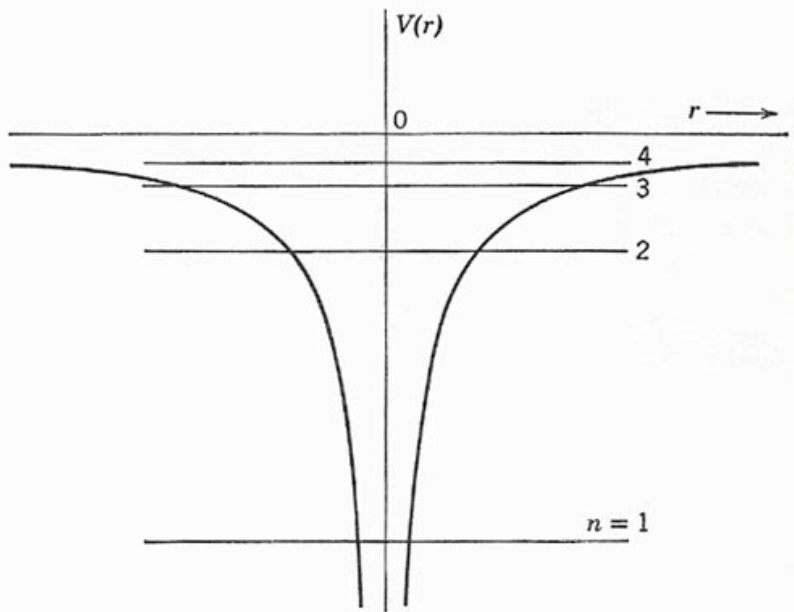
\includegraphics[scale=0.8]{Bilder/SamtaleTema3/Hydrogenatomet/hydrogenPot.png}
    \caption{Representasjon av potensialet til et hydrogenatom, r er radialle avstanden fra massesenteret.}
    \label{fig:hydro-pot}
\end{figure}

Hydrogenatomet har 3 kvantetall ($n$,$l$,$m$), bølgefunksjonen med polare koordinater kan derfor representeres som

\begin{equation}
    \psi_{lnm}(r,\theta,\phi)
\end{equation}

Der $n$ er det prinsipielle kvantetallet, $l$ er kvantetallet for angulær bevegelsesmengde (orbital kvantetall) og $m$ er det magnetiske kvantetallet.

\color{red}

\begin{itemize}
\centering
    \item $n$ relaterer til total energi
    \item $l$ relaterer til drivmoment (spinn)
    \item $m$ relaterer til z-komponenten til drivmomentet (hvilken retning den spinner)
\end{itemize}
\color{black}

\newpage
Kvantetallene kan inneha verdiene 

\begin{equation*}
    \begin{split}
        n &= 1, 2, 3, ...\\
        l &= 0, 1, 2, 3, ..., n-1\\
        m_l &= -l, -(l-1), ..., 0, ..., l
    \end{split}
\end{equation*}

En tilstand til hydrogenatomet med kvantetall $n=1$,$l=0$ og $m=0$ gir
$\psi_{100}$ osv. Dette gjelder kun for systemer med et elektron. 

For et system med et elektron vil energi nivå diagramet se ut som \href{https://www.google.com/search?q=energy+level+diagram+for+hydrogen&sca_esv=779b01740ca52ec5&sca_upv=1&rlz=1C5CHFA_enNO829NO829&udm=2&biw=1680&bih=904&sxsrf=ACQVn09akSWsMLxftMzmPMdTNcY0gxBSJA%3A1714049752819&ei=2FIqZpLKMbjPwPAP7-qYwAQ&oq=Energy+level+diagr&gs_lp=Egxnd3Mtd2l6LXNlcnAiEkVuZXJneSBsZXZlbCBkaWFncioCCAEyBRAAGIAEMgoQABiABBhDGIoFMgUQABiABDIKEAAYgAQYQxiKBTIFEAAYgAQyBRAAGIAEMgUQABiABDIFEAAYgAQyBRAAGIAEMgUQABiABEiVO1DKBVikKHAGeACQAQCYAfsBoAH7DaoBBjE2LjQuMbgBA8gBAPgBAZgCGKAC5A7CAgQQIxgnmAMAiAYBkgcGMTkuNC4xoAf_dw&sclient=gws-wiz-serp#vhid=NSb9L5eew_qdbM&vssid=mosaic}{Her}. Men når atomett har flere elektroner vil diagrammet forskyves litt, og det vil bli færre degenererte states. 

Madelungs regel går ut på at fylling av energinivåer går fra lavest til høyest verdi av $n+l$. Når to orbitaler har samme verdi for $n+l$, vil den med lavest $n$ bli fylt først. 

\subsection{Det periodiske systemet og Elektronkonfigurasjon}
\label{sec:tema3_4}
Det er mulig at to elektron opptar en energitilstand, en med spinn opp og en med spinn ned, det vil si at det er plass til to elektron per orbital. Dette henger sammen med mengde elektroner i atomer av forskjellige typer.

Vi ser på edelgasser som et eksempel. Neon [$He$] består av $2S^22P^6$, vi ser at åtteregelen er oppfylt i neon sitt tilfelle, skriver bare det i tillegg til forrige edelgass. Edelgaser har en ekstra stabil konfigurasjon.

Sannsynligheten for å finne et elektron i 1$S$-tilstanden har en radiell fordeling, altså en funksjon av avstanden fra sentrum. 

\begin{figure}[!htb]
    \centering
    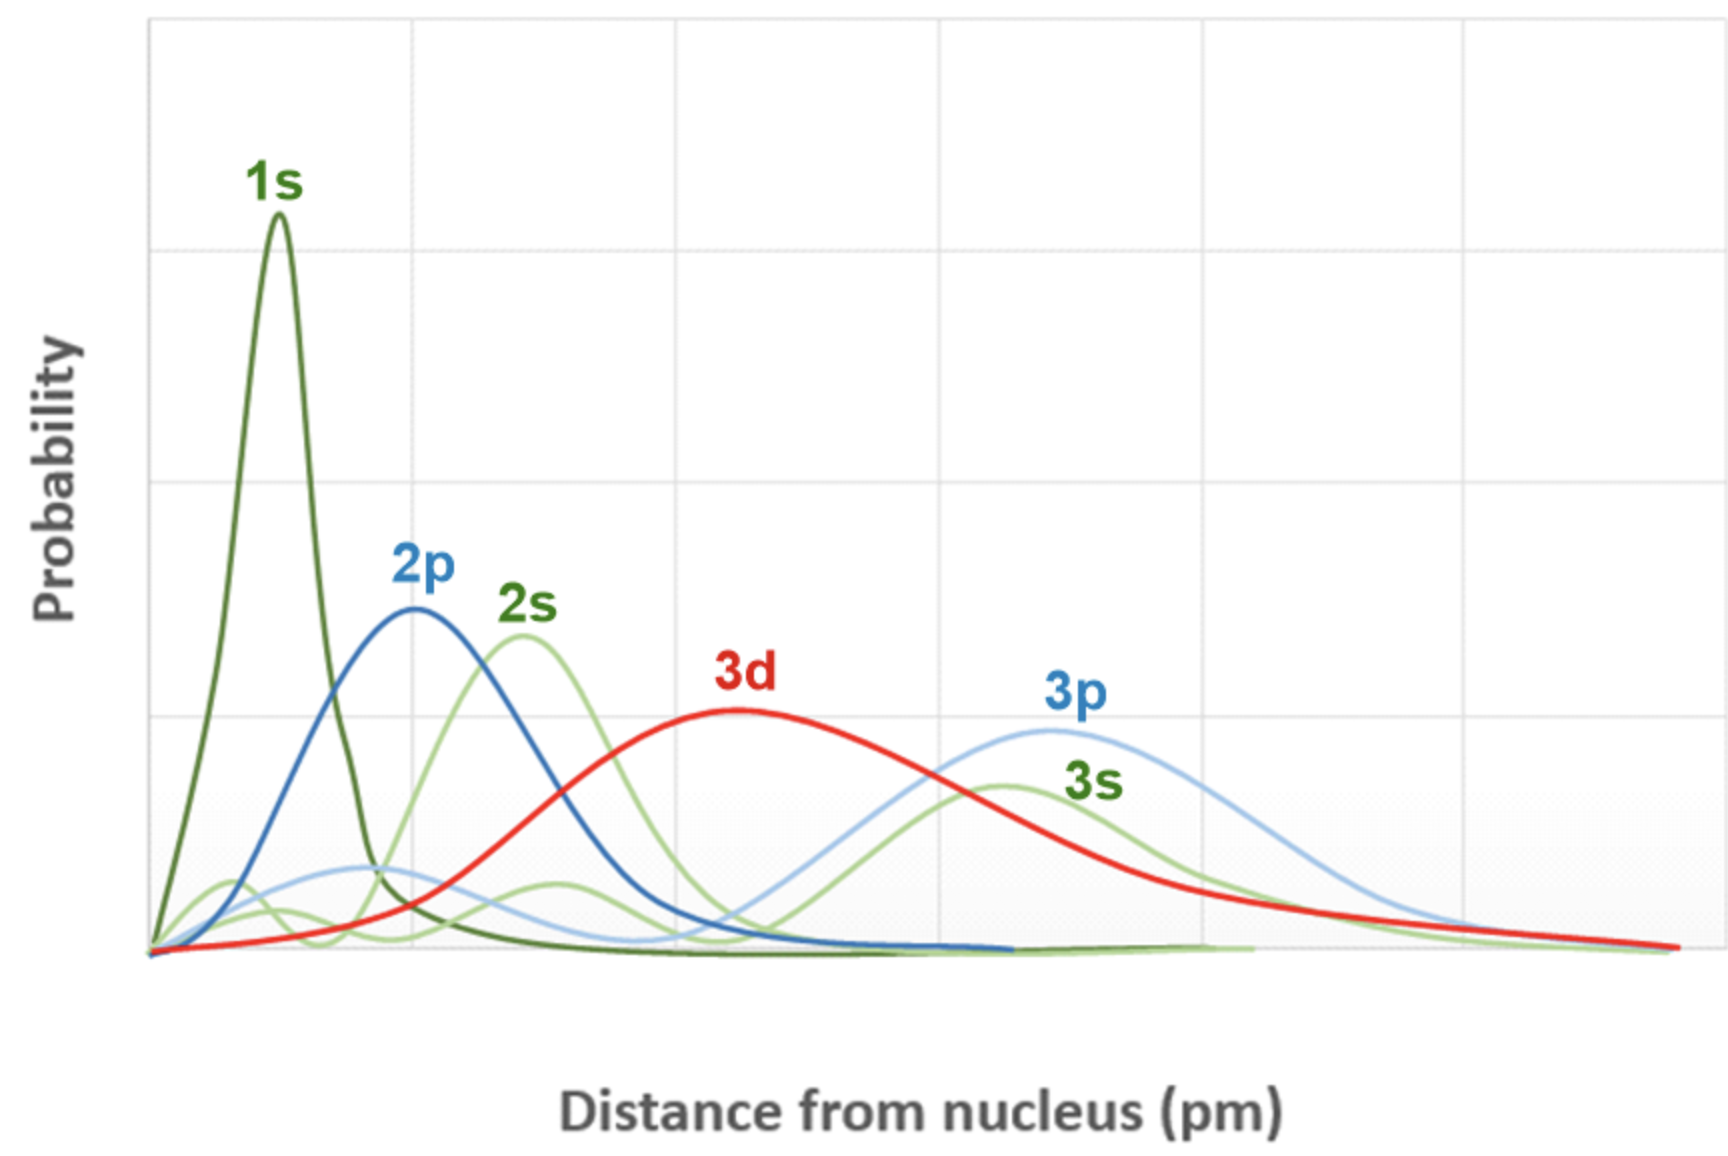
\includegraphics[scale=0.35]{Bilder/SamtaleTema3/InterPotens/radiellAvstand.png}
    \caption{Tilnærmet null sannsynlighet for noen av orbitalene å ha elektrone ved kjernen, vi ser at snitt verdien for avstand øker med økende orbital.}
    \label{fig:avstand}
\end{figure}

Orbitaler er nesten som en kompakt kule når alle ligger samlet og er flle, så et elektron som ligger i neste skall er ''ganske'' fritt.

Hund's regel sier at ''antall uparede elektroner (spinn opp/ned) er maksimert'' og ''Diisse uparede elektronene har egenskapen ''paralell spinn'', som medfører max total spinn i den ytterste orbitalen.''
Dette er fordi det å oppnå ulike orbitaler er ønskelig og energimessig, siden det reduserer gjensidig frastøtning og skjerming av atomkjernen. Med parallel spinn, har disse $e^-$ en null prosent sannsynlighet for å befinne seg i samme orbital, dette oppfyller Paulis eksklusjonsprinsipp.

\begin{figure}[!htb]
    \centering
    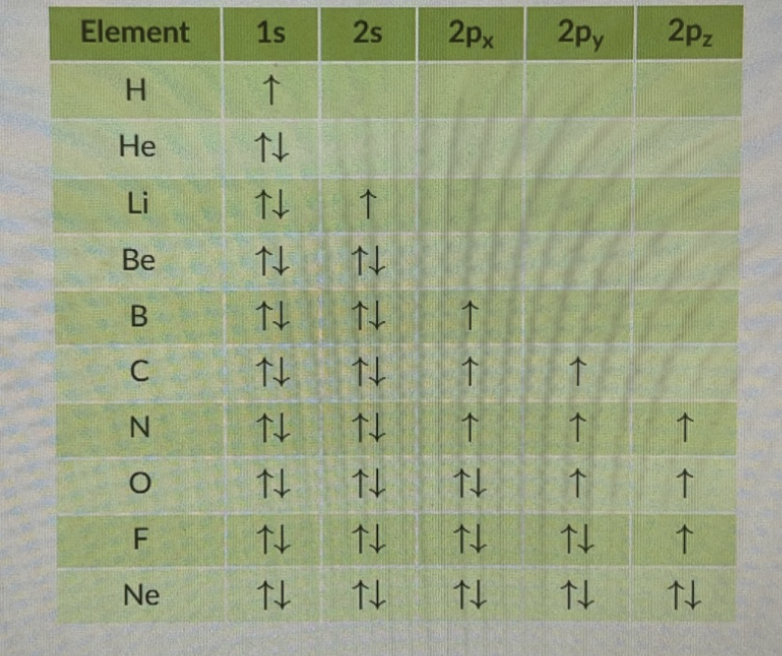
\includegraphics[scale=1]{Bilder/SamtaleTema3/box-arrow.png}
    \caption{Boks-pil diagram for de 10 første elementene i det periodiske system}
    \label{fig:box-arrow}
\end{figure}


\subsection{Bindinger i faste stoffer}
\label{sec:tema3_6}
Vi skal se på 3 viktige binder i denne underseksjonen, det er Ioniske bindinger, Metalliske bindinger og Koavalente bindinger.

Ioniske bindinger er veldig sterke bindinger, de er gode isolatorer fordi elektronkonfigurasjonen er veldig stabil. Bindingen er melom to ioner med motsatt ladning. Sterkere forskjell i elektronegativiteten gir en sterkere binding. I en ionisk binding er det ingen frie elektroner, dette gjør det som sagt til en dårlig leder, men en god isolator. vanlig sammensetning er ett atom med ett elektron i valensskallet, med ett som mangler ett for å oppnå edelgass konfigurasjon.

\begin{figure}[!htb]
    \centering
    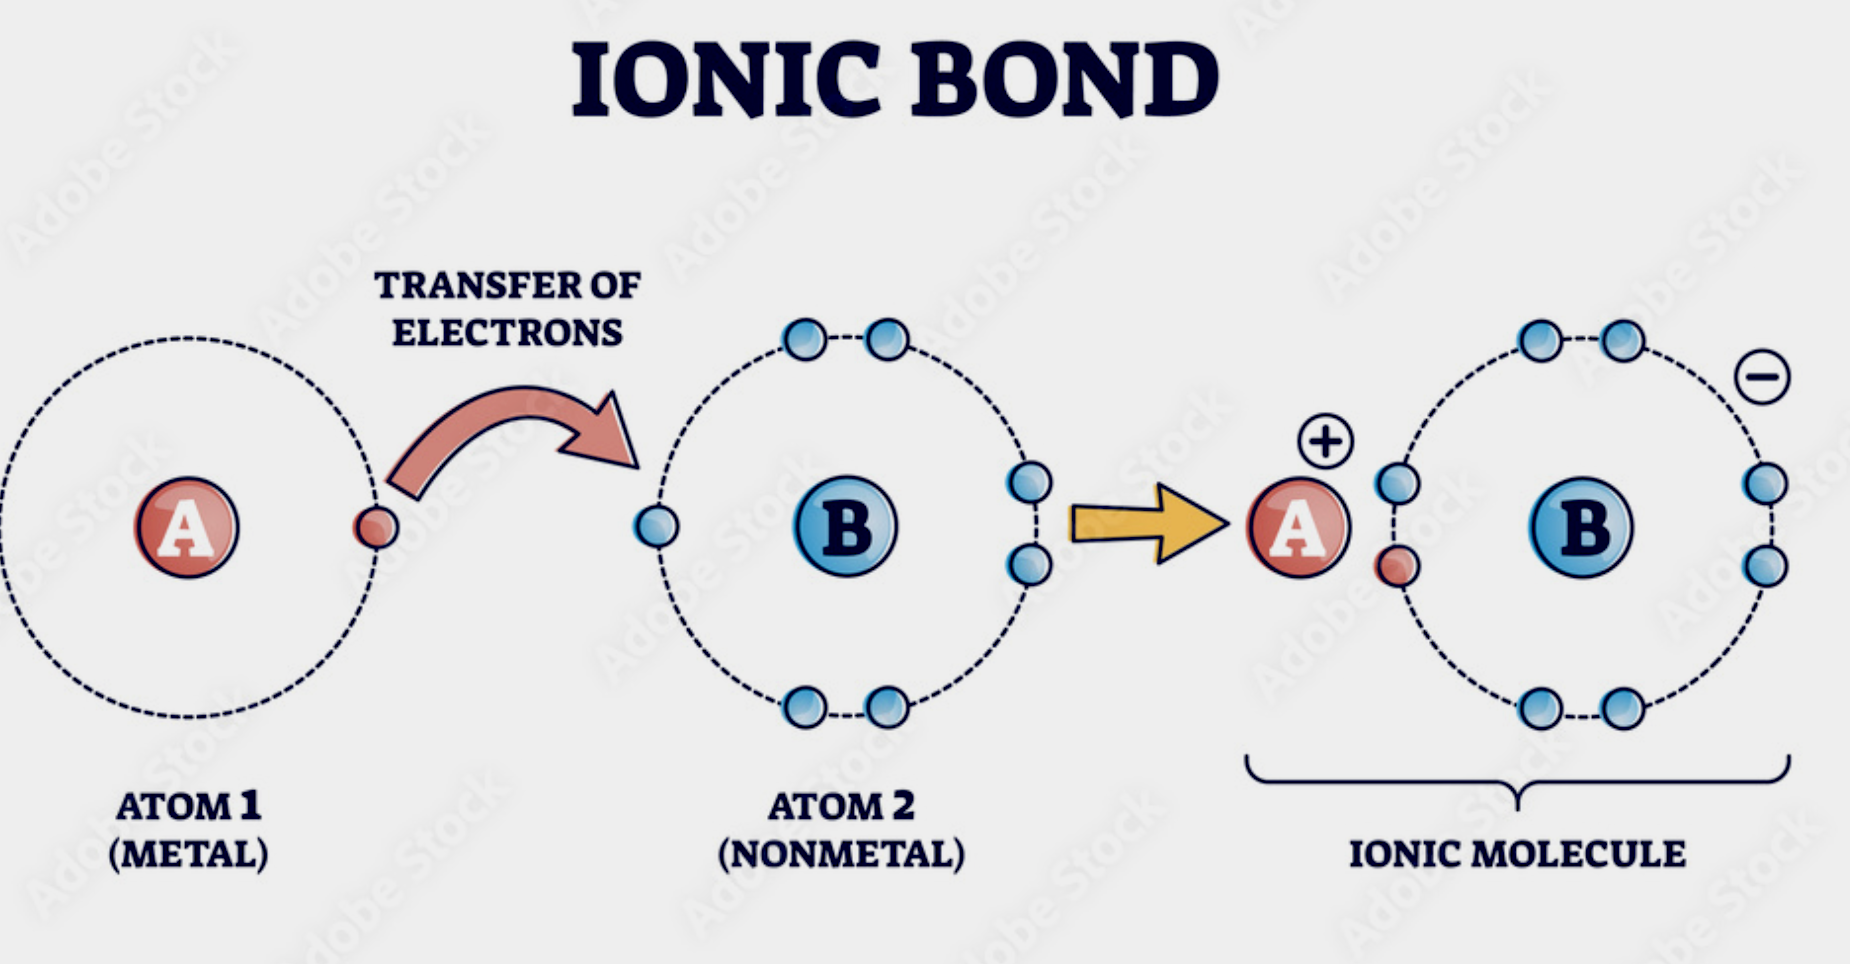
\includegraphics[scale=0.4]{Bilder/SamtaleTema3/Bindinger/ionic.png}
    \caption{Ionisk binding}
    \label{fig:ione}
\end{figure}

Metalliske bindinger er bindinger som oppstår i metaller, de er typisk gode til å lede. Bindingene oppstår mellom atomer med lav elektronegativitet, det holder metaller sammen. Man sier ofte at metall atomene er omgitt av et elektronhav der atomer ikke holdes fast av de andre atomene, men av elektronsjøen. Metaller er gode ledere nettop pga. dette, elektronene er ikke fastbundne, så de har en relattivt fri flyt. Dette er bindinger som ikke er like sterke som iioniske og koavalente bindinger. 

\begin{figure}[!htb]
    \centering
    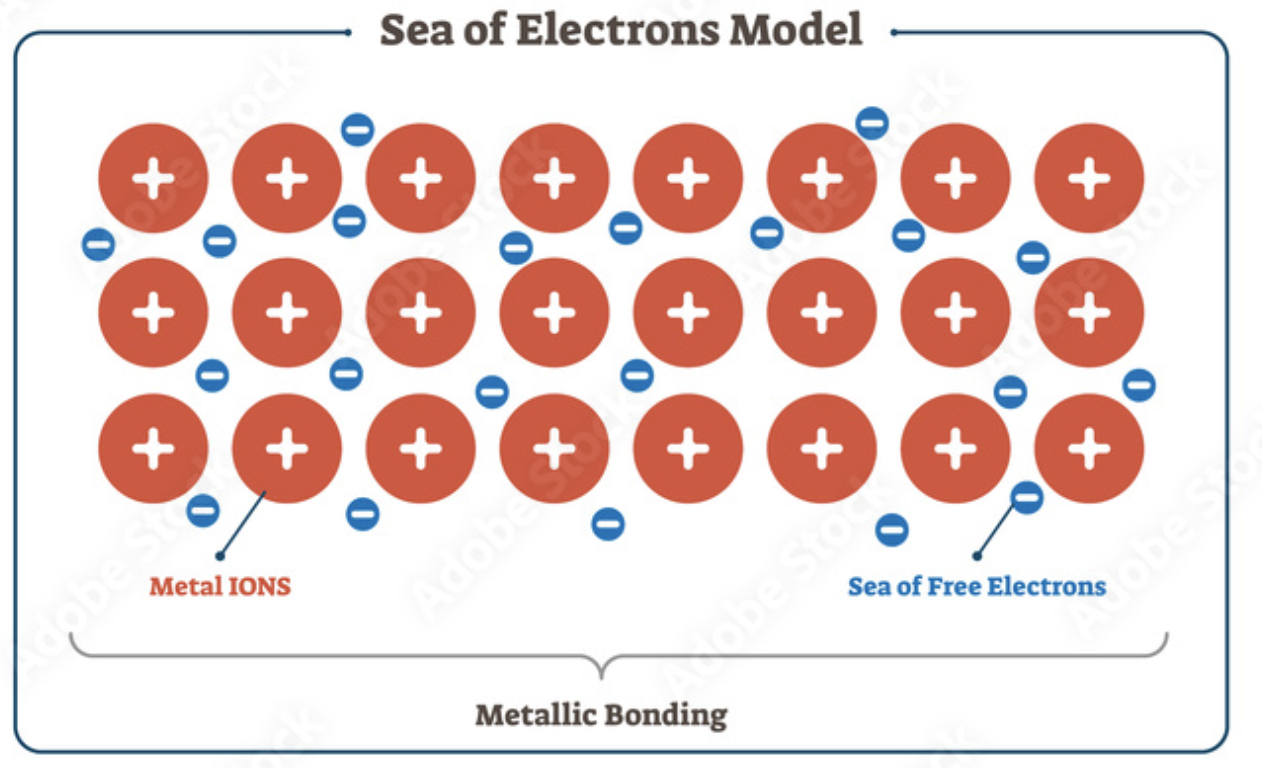
\includegraphics[scale=0.4]{Bilder/SamtaleTema3/Bindinger/metallic.png}
    \caption{Elektronsjø representasjon av metalliske bindinger}
    \label{fig:metallisk}
\end{figure}

Koavalente bindinger, oppstår ofte i halvledere, de er bistabile mellom å være en leder og en isolator. Koavalente bindingener oppstår mellom to molekyler som deler et elektronpar. Dette kan være enkelt, dobbelt eller trippelbinding. Det har dårlig ledningsevne da elektronene for det meste er lokalisert mellom atomene. Det er sterke bånd, men med kort båndlengde. 

Koavalente bindinger oppstår ofte når alle mangler ett eller flere elektron for edelgasskonfigurasjon, ved å bryte mange bindinger vil det lede bedre og bedre. 

\begin{figure}[!htb]
    \centering
    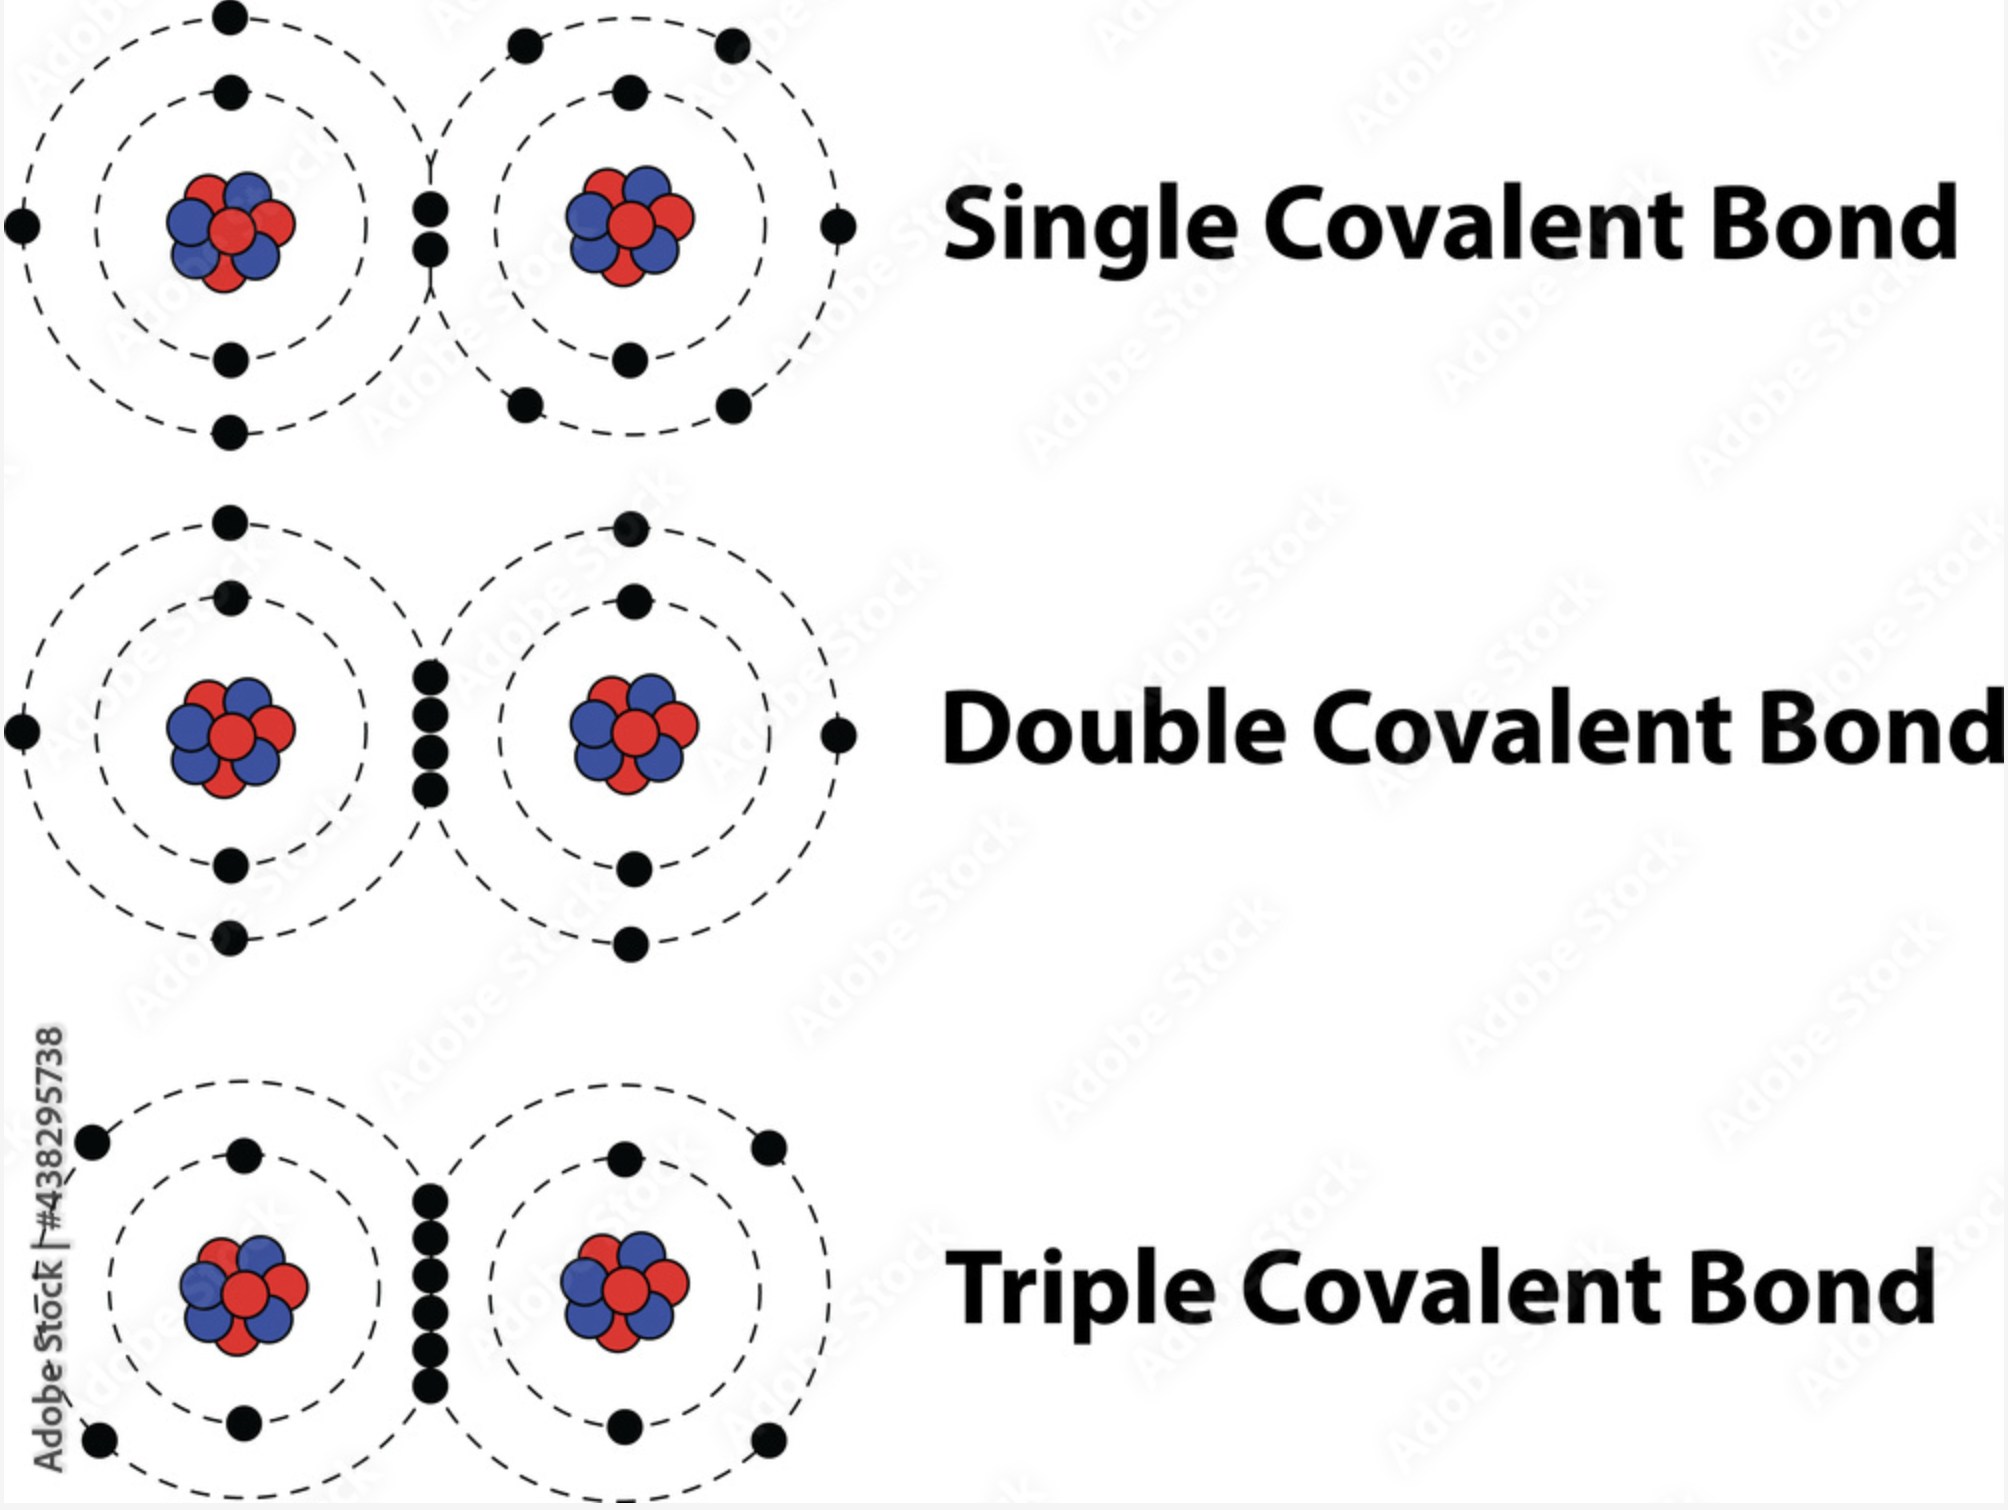
\includegraphics[scale=0.3]{Bilder/SamtaleTema3/Bindinger/covalent.png}
    \caption{enkel, dobbel og trippel covalent binding}
    \label{fig:cov}
\end{figure}

\subsection{Dobbel kvantebrønn}
\label{sec:tema3_7}
Vi har til nå sett på kvantebrønn i 1D, dette har vi sett på som en forenklet modell av hydrogenatomet, men vi vil gjerne introdusere mer kompleksistet så vi kan jobbe med mer enn bare et elektron og et proton. Vi legger til et proton i kjernen til Hydrogen atomet og får $H_2^+$, dette kan vi se på som to brønner som står ved siden av hverandre. 

Ved å føre to brønner sammen, der begge er i grunntilstand får vi figur \ref{fig.dobbelB}

\begin{figure}[!htb]
    \centering
    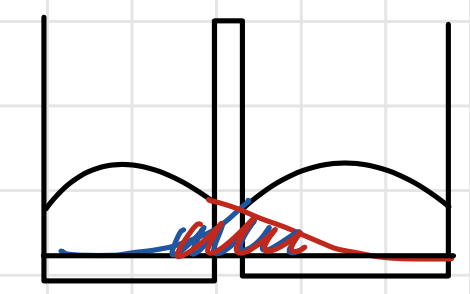
\includegraphics[scale=1]{Bilder/SamtaleTema3/DobbelBrønn/dobbelBrønn.png}
    \caption{To enkelt brønner lagt sammen til en dobbelbrønn, $\psi_1$ og $\psi_2$. Det skraverte området er en del av løsningen som bryter med Paulis eksklusjonsprinsipp.}
    \label{fig:dobbelB}
\end{figure}

Siden atomene er tett på hverandre, og barrieren mellom dem ikke er uendelig høy eller ''langt unna'', kan bølgefunksjonen tunnellere gjennom og lekke over til motsatte side. Problem når bølgefunksjonene tar pass på sted pga. Paulis eksklusjonsprinsipp.

Vi har hvertfall en superposisjon av tilstandene

\begin{equation*}
    \begin{split}
    \psi_B &= \psi_1 + \psi_2\\
    \psi_A &= \psi_1 - \psi_2
    \end{split}
\end{equation*}

Disse er begge gyldige løsninger på SL. Å sette sammen to atomer slik endrer grunntilstanden (de gror sammen, danner enten en sum eller differanse). Den som har lavest energi og som dermed blir den nye grunntilstanden er $\psi_B$ siden den har mindre krumming, den dobbelderiverte er mindre. \autoref{fig:solDobbel} viser hvordan grunntilstanden og første eksiterte tilstand vil se ut.

\begin{figure}[!htb]
    \centering
    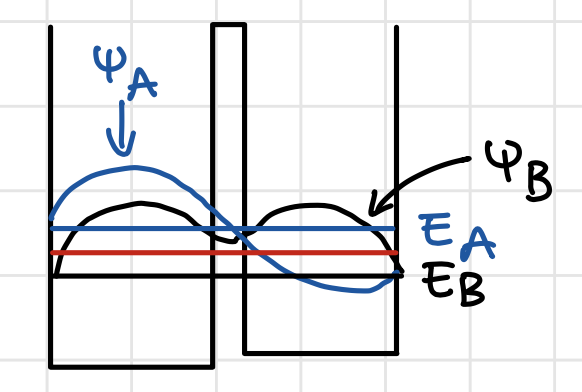
\includegraphics{Bilder/SamtaleTema3/DobbelBrønn/solDobbel.png}
    \caption{Røde linjen er energien til den gamle bølgefunksjonen.}
    \label{fig:solDobbel}
\end{figure}

$\psi_B$ har subskriptet B da det står for bonding orbital, det er bølgefunksjonen som indikerer en binding mellom to atomer. Den senker $E$, mer gunstig for systemet å være her. Det ligner på et kovalent bånd.

$\psi_A$ har subskript A da det står for Anti bonding orbital, den hever energien og den har lav $|\psi_A|^2$ mellom atomene. 

Barriere har noe å si, jo høyere energinivåer desto lettere å tunnellere gjennom barrieren (mye lekkasje). Tilstandene med mindre energi ser en større barriere og sannsynligheten for at de tunnellerer er liten.

Lavt energinivå betyr at atomene er langt fra hverandre, høyere er da nærmere, og de har stor energi i forhold til høyden på brønnen, det vil si større lekkasje da det skal mindre til å tunnellere.

\subsection{Det interatomære potensiale}
\label{sec:tema3_8}
Det interatomære potensialet referer til den potensielle energien mellom to eller flere atomer. Den oppstår som følge av interaksjoner mellom de tilhørende partiklene som elektroner og protoner/nøytroner.

Oppsummert er det energien som to eller flere atomer har pga. en gjensidig tiltrekning/frastøtning. Potensialet påvirker hvordan atomer interagerer og bindes sammen.

\begin{figure}[!htb]
    \centering
    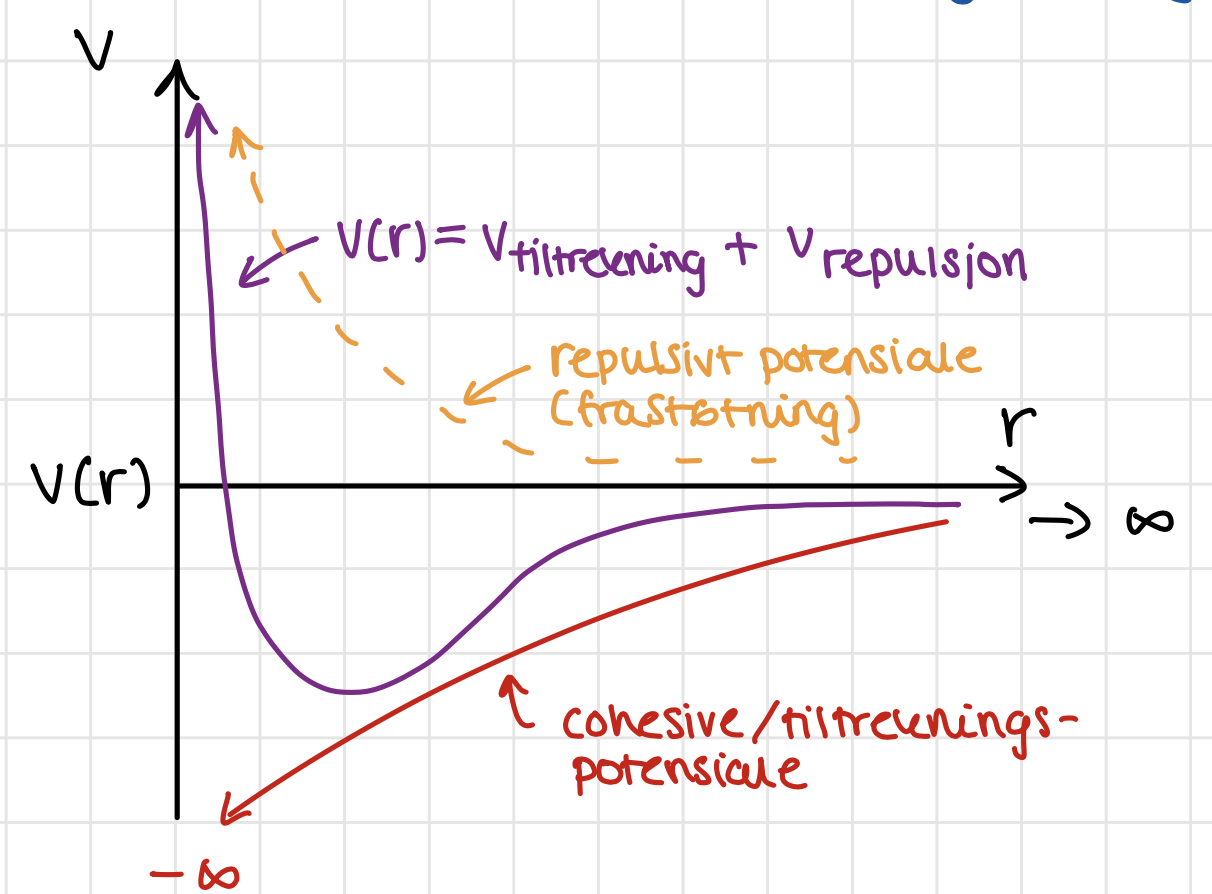
\includegraphics[scale=0.6]{Bilder/SamtaleTema3/InterPotens/Ipot.png}
    \caption{Interatomær energikurve for potensiell energi, en funksjon av den radielle avstanden $r$.}
    \label{fig:Ipot}
\end{figure}

Vi bruker $r$ i figur \ref{fig:Ipot} fordi vi antar at atomer og ioner er radielt symmetriske. Med det er $r$ avstanden mellom atomene. 

Det er mulig å si at to atomer langt unna hverandre ser hverandre, og vil i realiteten alltid påvirke hverandre, men den potensielle energien er tilnærmet null når man er langt unna. 

Tenker vi på atomer med ulike orbitaler, vil de ikke at orbitalene skal overlappe for mye, Dette er ofte forklart med Paulis eksklusjonsprinsipp, men essensielt så er det en energi som hindrer overlappen.

\newpage

\section{Tema 4: Krystallografi og resiprokt rom}
\label{tema4}

\begin{table}[!htb]
    \centering
    \caption{Samtale punkter tema 4}
    \begin{tabular}{|c|c|c|r|}
      \hline
      1 & Faste stoff \& Krystaller, basis og gitter &  \autoref{sec:tema4_1} & \cellcolor{green}\quad\quad \\
      \hline 
      2 & Enhetsseller & \autoref{sec:tema4_3} & \cellcolor{green} \\
      \hline
      3 & Wigner-seitz celle & \autoref{sec:tema4_7} & \cellcolor{green} \\
      \hline 
      4 & Kubiske gitter (fcc, bcc, sc) & \autoref{sec:tema4_5} & \cellcolor{green} \\
      \hline
      5 & Miller indekser & \autoref{sec:tema4_6} & \cellcolor{green} \\ 
      \hline
      6 & Reelt og Resiprokt rom/gitter & \autoref{sec:tema4_8} & \cellcolor{blue} \\
      \hline
    \end{tabular}
    \label{tab:samtalePunkt_tema1}
\end{table}

\subsection{Faste stoff \& Krystaller, basis og gitter}
\label{sec:tema4_1}
Faser er en måte å beskrive tilstanden til stoffer, vi har gass, væske og fast form. Vi ser på faste stoffer, dermed er det mest interessant å se på fast form. Fast form kan deles inn i ordnet og uordnet, der ordnet betyr regelmessig arrangement av atom (langt-rekkende ordning) eller krystallinsk tilstand. For uordnede faste stoffer vil atomene ha en tilfeldig ordning, som er en kortrekkende ordning. 

\begin{definition}
    \textbf{Langt-rekkende}. Ved å se hvordan utformingen til et stoff er i (relativt) kort rekkevide, kan man vite hvordan det ser ut langt unna.
\end{definition}

\begin{figure}[!htb]
    \centering
    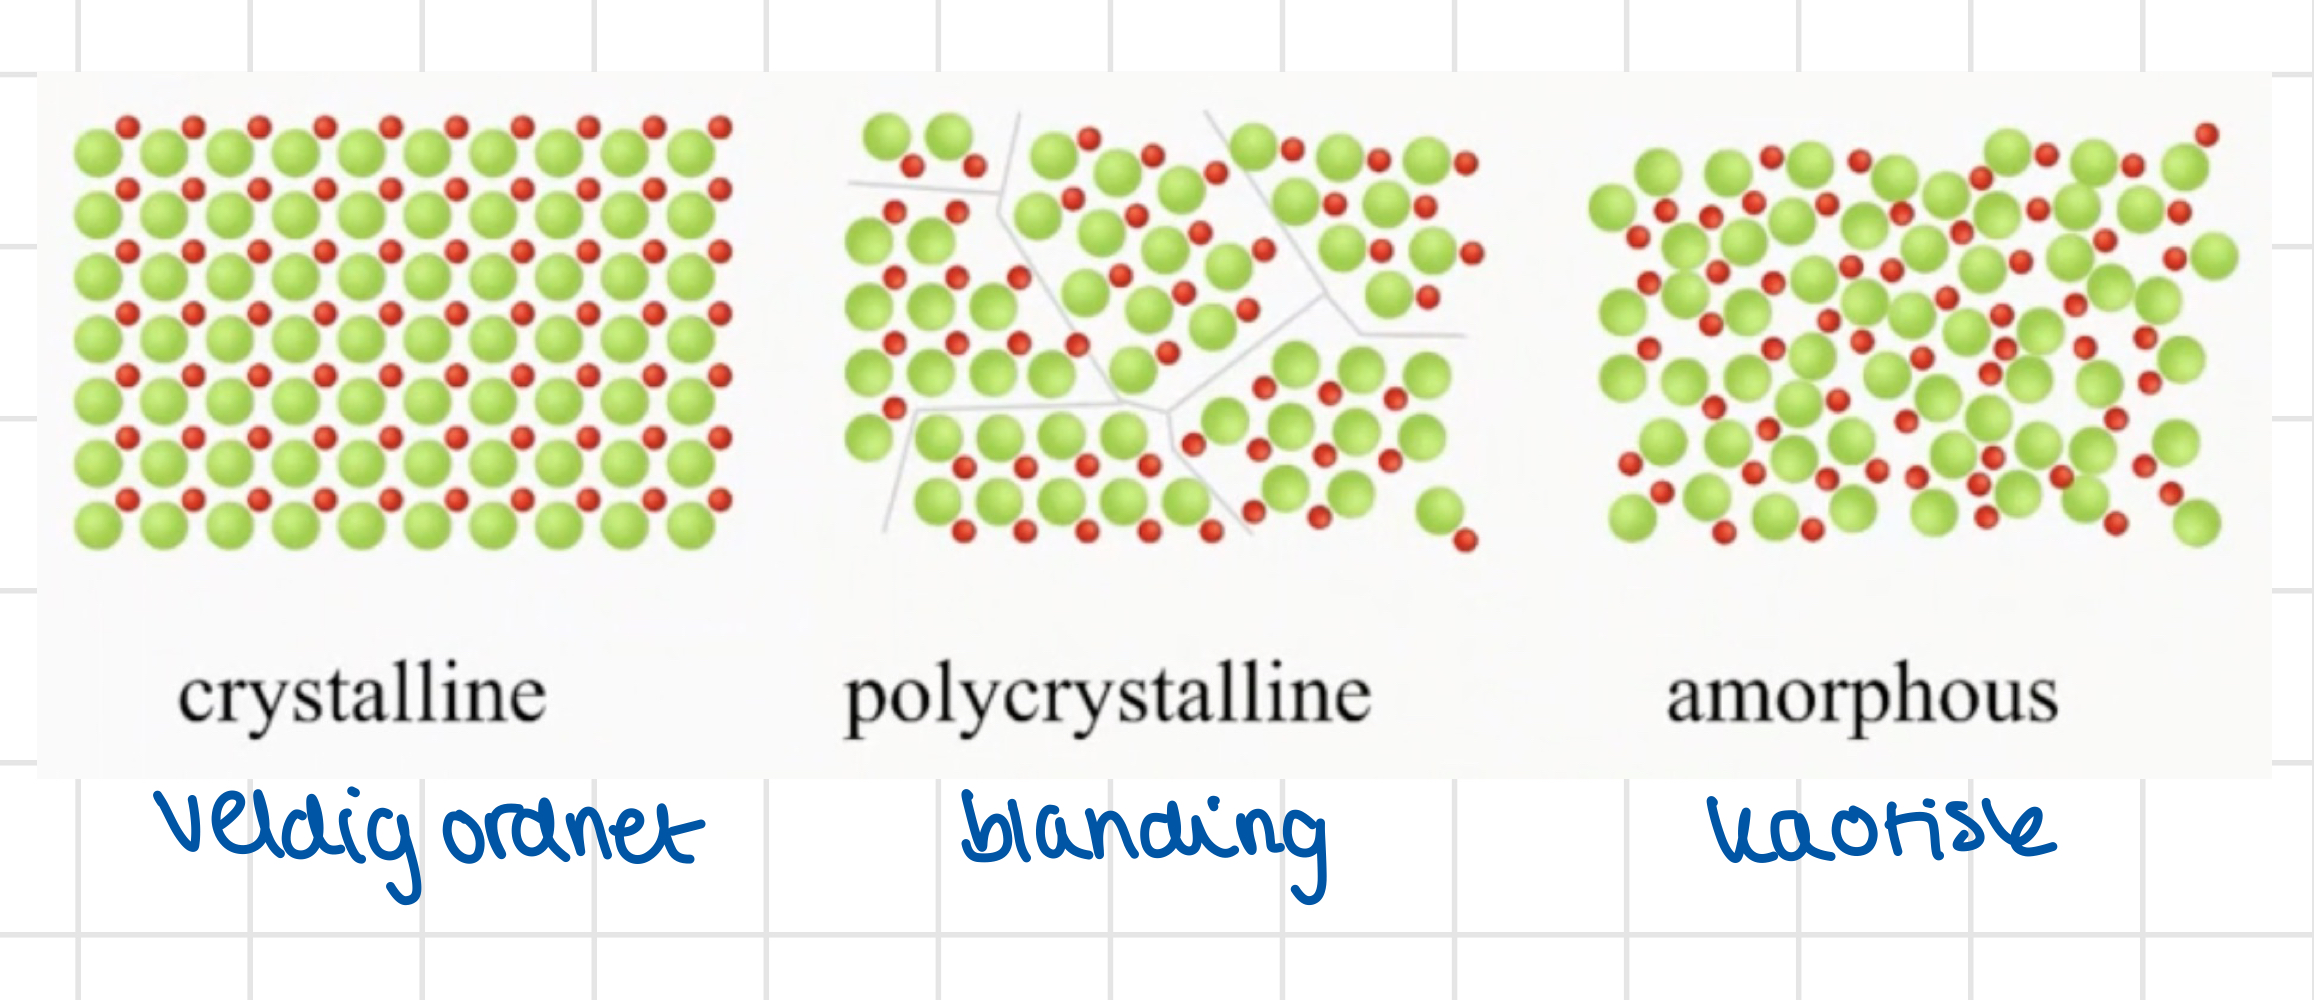
\includegraphics[scale=0.2]{Bilder/SamtaleTema4/Faste Stoffer/faserr.jpeg}
    \caption{Krystallinsk tilstand er veldig ordnet, mens polykrystallinsk delvis ordnet, men amorft er helt kaotisk}
    \label{fig:EskempelOppbygning}
\end{figure}

For å kunne forklare hvordan et stoff er bygget opp kan det være nyttig å innføre den anvendte terminologien. En krystall er satt sammen av en basis og et gitter. \autoref{fig:cryst} viser at basis pluss gitter gir ut krystall. Et gitter er kun et samling matematiske punkt i rommet for å hjelpe oss med å beskrive et stoff. Basisen brukes til å fortelle om sammensetning av atomer som festes til hvert gitterpunkt.

\begin{figure}[!htb]
    \centering
    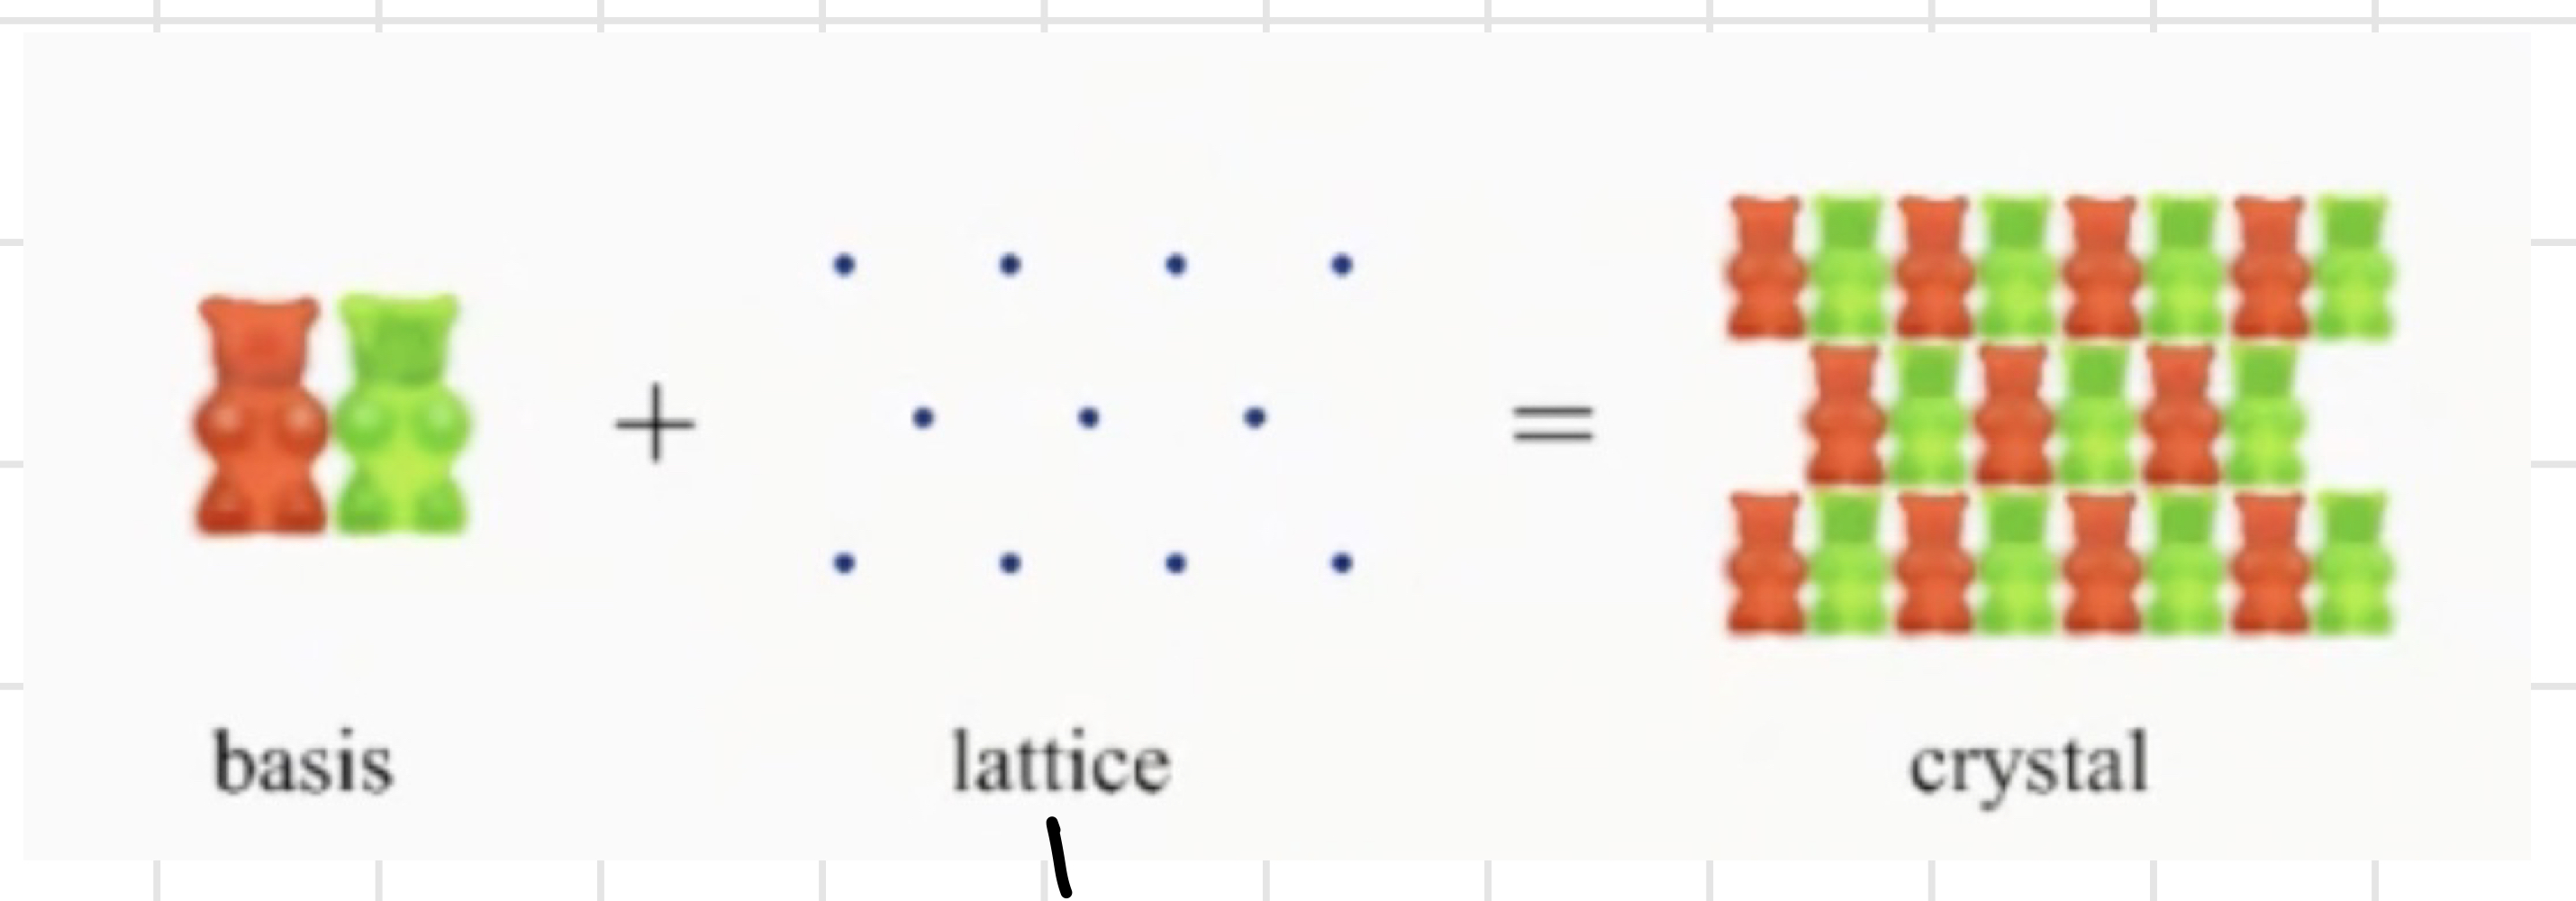
\includegraphics[scale=0.15]{Bilder/SamtaleTema4/Faste Stoffer/krystallKlosser.jpeg}
    \caption{Krystaller er satt sammen av en basis som legges på hvert gitterpunkt (latticepoint)}
    \label{fig:cryst}
\end{figure}

\begin{definition}
    \textbf{Enhetscelle}: er den minste byggeklossen som beskriver gitteret.
\end{definition}

\subsection{Enhetsseller}
\label{sec:tema4_3}
Et gitter kan representeres matematisk i reelt rom,

\begin{equation}
\label{eq:real}
    \Vec{R} = \sum_{i=1}^3 n_i\Vec{a_i},
\end{equation}

Her er $n_i$ positive eller negative heltall som skalerer vektorene $a_i$ i rommet, disse kan også være null. $a_i$ er enhetsvektorene som beskriver gitteret.

\begin{definition}
    \textbf{Bravaisgitter}: 3-dimensjonal konfigurasjon som atomer kan bli arrangert innenfoor krystaller.
\end{definition}

Det finnes 14 typer bravaisgitter som beskriver enhver krystall. \MYhref{https://en.wikipedia.org/wiki/Bravais_lattice}{Wikipedia} viser alle 14 for tre dimensjonelt rom, og 5 for to dimensjonelt.

\begin{definition}
    \textbf{Enhetscellen}: Den minste byggeklossen som beskriver et gitter. Enhetscellen kan ikke ha \textit{ikke periodiske} former.
\end{definition}

Vi kan dele enhetsceller inn i to kategorier, primitive og konvensjonelle. Primitive enhetsceller inneholdeer bare ett gitterpunkt. Konvensjonelle enhetsceller er vanlige konfigurasjoner og kan inneholde mer enn ett gitterpunkt. Det er oftere enklere å finne konvensjonelle enhetsceller. Men vi skal nå se på en systematisk måte å produsere en enhetscelle.

\subsection{Wigner-seitz celle}
\label{sec:tema4_7}
Wigner-Seitz cellen er en bestemt måte å finne en primitiv enhetscelle på. WS-cellen produseres ved å konstruere vektorer fra et gitt gitterpunkt til ''alle andre'' gitterpunkt, for deretter å konstruere linjer (2D) eller plan (3D) på midtpunktet av vektorene.

Kanten av en WS-celle ligger alltid halveis mellom to rekker med atomer. 

\begin{figure}[!htb]
    \centering
    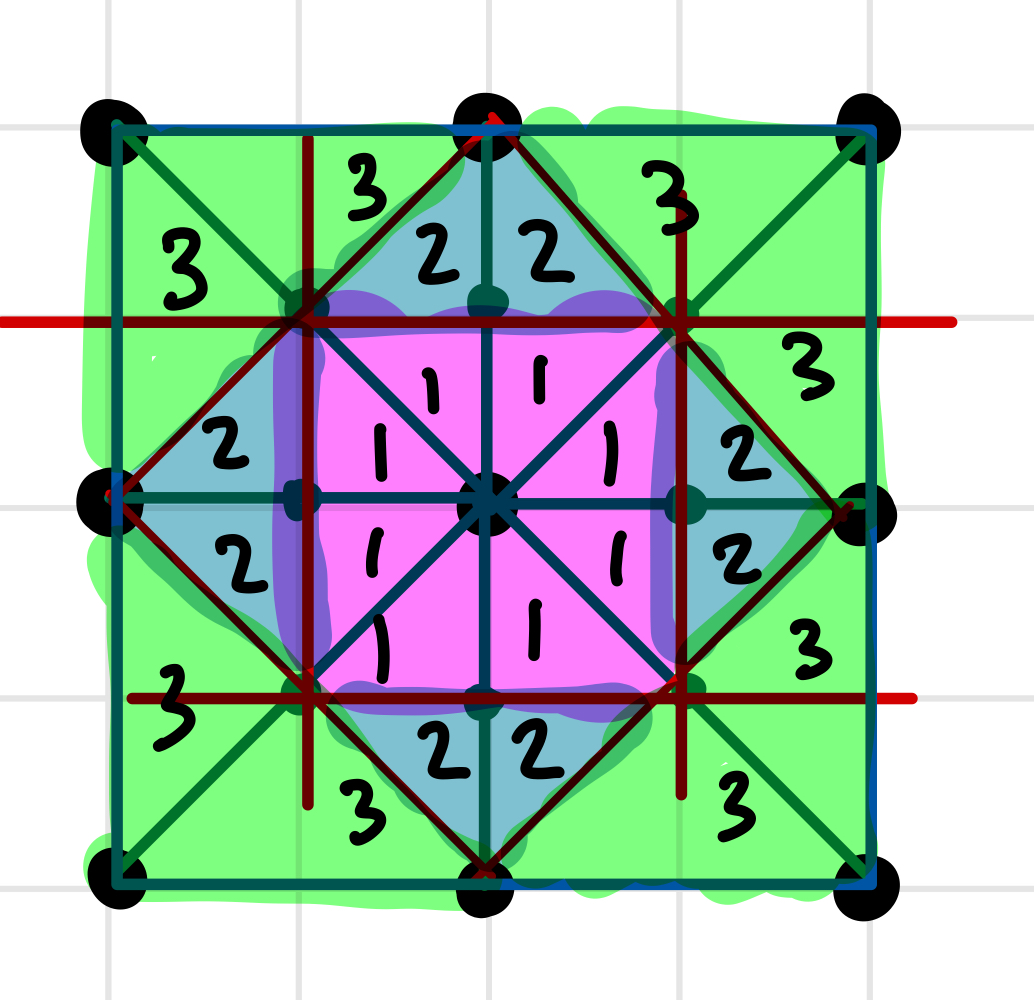
\includegraphics[scale=0.2]{Bilder/SamtaleTema4/WS_Celle.jpeg}
    \caption{Wigner-Seitz cellen, første orden i \color{purple}lilla\color{black}, andre orden \color{blue}{blå} \color{black} og tredje orden i \color{green}{grønn}\color{black}.}
    \label{fig:enter-label}
\end{figure}

\subsection{Kubiske gitter (sc, fcc, bcc)}
\label{sec:tema4_5}
Gitterpunktene til en simple cubic (sc) enhetscelle kan forklares med en tre dimensjonell tegning. Lengdene på alle sidene er like lange, så orienteringen i rom har ikke noe å si for enhetscellen. Som en vanlig er det tre vektorer som møtes til hvilket som helst punkt på kuben, vinkelen mellom disse vektorene er 90$^\circ$. I en sc enhetscell er det totalt ett atom per enhetscelle, det fordeles slik

\begin{equation*}
    \frac{1}{8}\cdot 8 = 1,
\end{equation*}

$\frac{1}{8}$ kommer av et hvert atom deles med \textbf{syv} nabo sc-enhetsceller. 

\begin{figure}[!htb]
    \centering
    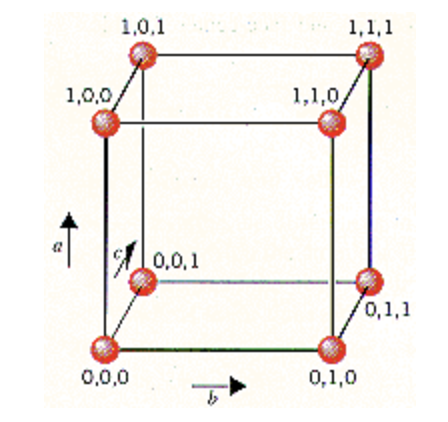
\includegraphics[scale=0.8]{Bilder/SamtaleTema4/sc.png}
    \caption{En simple cubic enhetscelle}
    \label{fig:sc}
\end{figure}
\newpage
Face centered cubic (fcc) er en konfigurasjon mye lik som sc, men i tillegg til hjørnene så er det atomer på hver flate av kuben. Denne enhetscellen har det vi kaller høyest pakketetthet, det vil si at atomene tar opp størst volum av kuben, av de tre enhetscellene vi går inn på. Antall atomer i en fcc er 

\begin{equation*}
    \frac{1}{8} \cdot 8 + \frac{1}{2}\cdot 6 \,= \,4
\end{equation*}

Faktoren på en halv representerer at flatsidene på cellen deles med en identisk celle, dermed får begge ''eierskap'' på halve volumet til atomet og en kube har seks sider.

\begin{figure}[!htb]
    \centering
    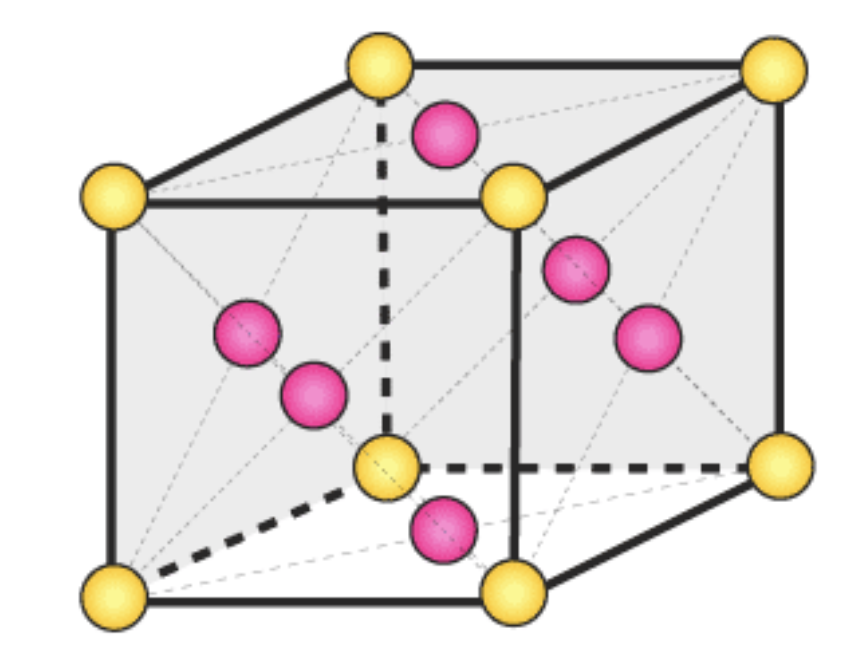
\includegraphics[scale=0.5]{Bilder/SamtaleTema4/fcc.png}
    \caption{Face centered cubic unitcelle.}
    \label{fig:fcc}
\end{figure}

Body centered cubic (bcc) er en enhetscellen akkurat som fcc, som har byggekloss sc i grunn, også finnes det da som navnet tilsier body centered. Et punkt i kjernen av kuben. Dette medfører at totalt antall atomer for en bcc er

\begin{equation*}
    \frac{1}{8}\cdot 8 + 1 = 2
\end{equation*}

\begin{figure}[!htb]
    \centering
    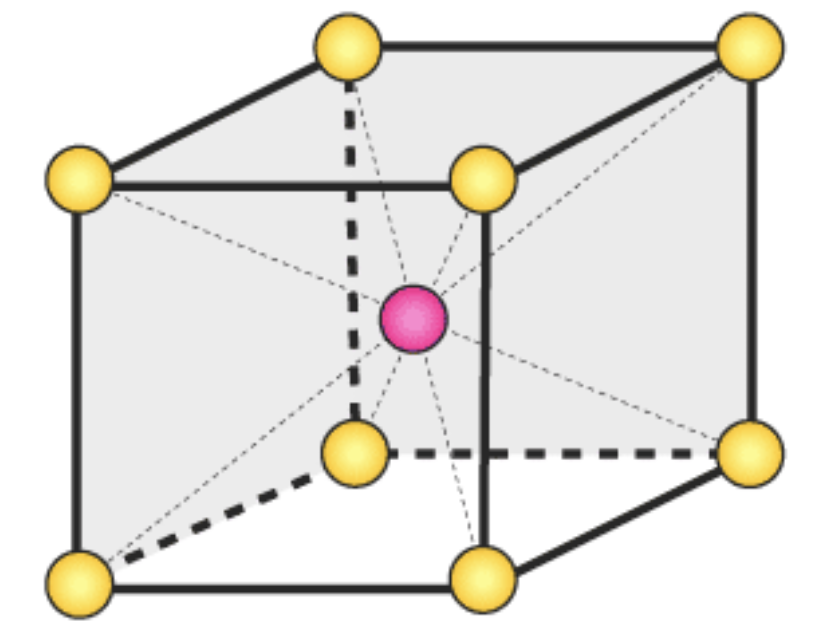
\includegraphics[scale=0.5]{Bilder/SamtaleTema4/bcc.png}
    \caption{Boody centered unit cell}
    \label{fig:bcc}
\end{figure}

\subsection{Miller indekser}
\label{sec:tema4_6}
Miller indekser brukes for å angi retninger i en krystall. Dette er nyttig siden krystaller er an-isotropiske, altså de er ikke like i alle retninger, så avhengig av hvordan du måler de vil krystallen se forskjellig ut og dermed ha forskjellige oppførseler. \autoref{fig:miller} viser alle millerindeksene.

\begin{figure}[!htb]
    \centering
    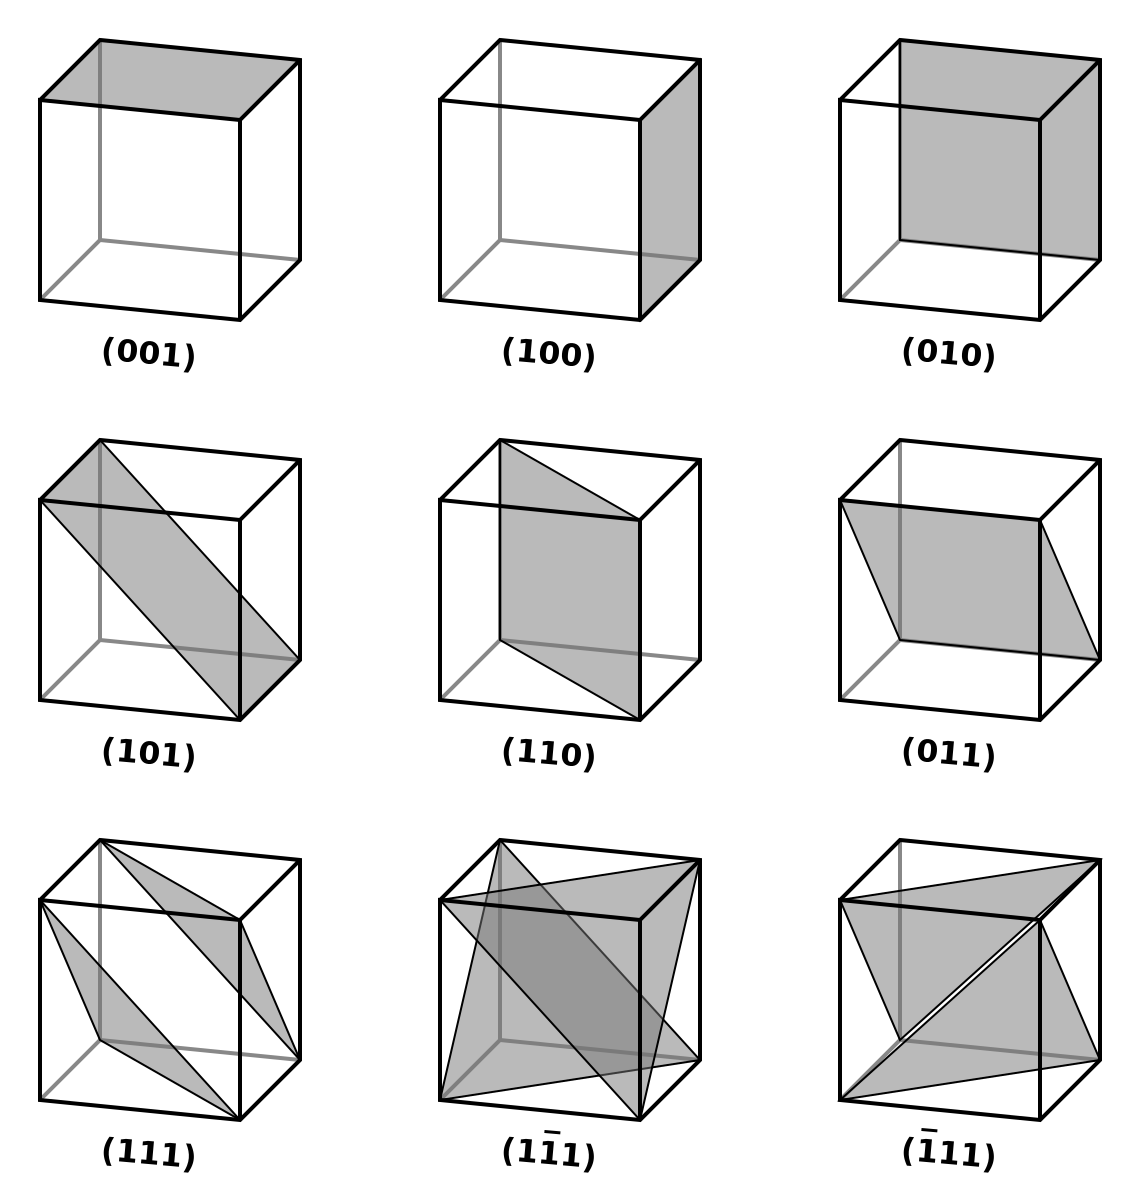
\includegraphics[scale=0.3]{Bilder/SamtaleTema4/miller.png}
    \caption{Alle miller indeksene, bar over tall er en annen notasjon for minus.}
    \label{fig:miller}
\end{figure}

Git et plan, så er det relativt lett å finne Miller indeksen. La oss ta utgangspunkt i indeksen øverst til venstre, $x$ er definert positivt høyre, $y$ inn i arket og $z$ oppover. 

Vi ser at $z$-aksen blir skjært, men $y$- og $x$-aksen går mot uendelig, dermed får vi 

\begin{equation*}
    (\infty \; \infty \; 1) \implies \bigg(\frac{1}{\infty}\;
    \frac{1}{\infty}\; \frac{1}{1}\bigg) = (0\;0\;1)
\end{equation*}
 \newpage
 
\subsection{Reelt og Resiprokt rom/gitter}
\label{sec:tema4_8}
Fourier transformen er mye brukt i signalanalyse, da den gir et forhold mellom et signal og tilhørende frekvenser i signalet. Fourier transformen tar et signal og splitter det i sine respektive komponenter. Mindre verdier i tidsdomenet gir høyere verdier i frekvensdomenet. Dette gjelder også for rom, vi sier derfor at resiprokt rom er Fourier transformen av reelt rom.

\begin{equation}
    \mathscr{F}(\mathbb{R}^n) = \text{Resiprokt rom},
\end{equation}

Vi kan med det si at gitter er romlige frekvenser som Fourier transformeres. I reelt rom har vi i en dimensjon $x$ for avstand, mens i resiprokt rom blir dette $\frac{1}{x}$. I en tre dimensjonell situasjon får vi da frekvenser i flere dimensjoner. Diffraksjon kan benyttes for forståelse av dette. 

\begin{figure}[!htb]
    \centering
    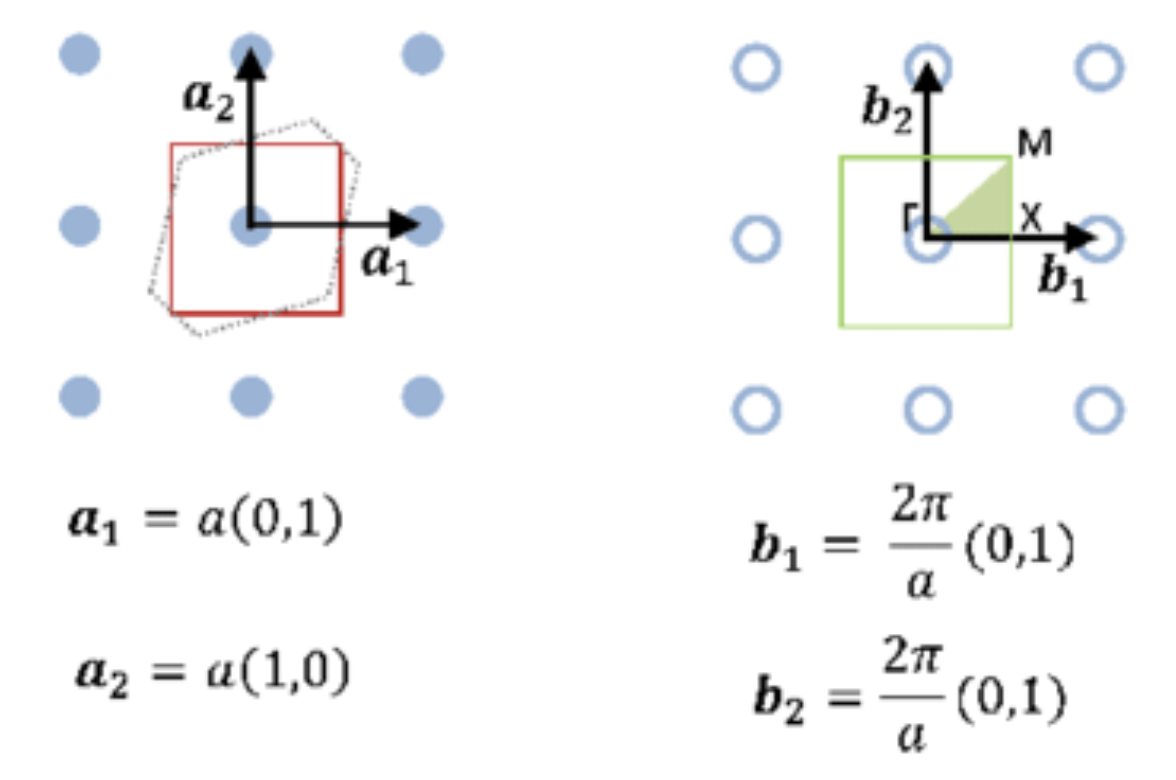
\includegraphics[scale=0.4]{Bilder/SamtaleTema4/resip.png}
    \caption{Overgangen fra reelt rom til resiprokt rom, faktoren $2\pi$ er en konsekvens av Fourier transformen.}
    \label{fig:resip}
\end{figure}

Vi har vært gjennom sc, fcc og bcc. Det skjer noe interesant når vi Fourier transformerer disse.

\begin{equation*}
    \begin{split}
        \textbf{sc} &\xrightarrow{\mathscr{F}} \textbf{sc}\\
        \textbf{fcc} &\xrightarrow{\mathscr{F}} \textbf{bcc}\\
        \textbf{bcc} &\xrightarrow{\mathscr{F}} \textbf{fcc}\\
    \end{split}
\end{equation*}

I motsetning til relle gittervektorer som kan beskrives med ligning \ref{eq:real}, så beskrives resiproke gittervektorer annerledes, blandt annet ved hjelp av MillerIndeksene.

\begin{equation}
    \label{eq:resiprok}
    \Vec{G}_{hkl} = h\Vec{b}_1 + k \Vec{b}_2 + l \Vec{b}_3,
\end{equation}

Eventuelt kan de skrives på formen 
\begin{equation}
\label{eq:resiprok2}
    \Vec{G}_{hkl} = \frac{2\pi \Vec{n}_{hkl}}{d_{hkl}}
\end{equation}

I ligning \ref{eq:resiprok2} er $\Vec{n}_{hkl}$ normalvektoren til Miller planet, og $d_{hkl}$ er den inter-planære avstanden, det vil si avstanden parallelt mellom to plan.

En rotasjon mellom reelle og resiproke basisvektorer kan beskrives med en syklisk permutasjon:

\begin{equation}
\label{eq:syklisk}
    \begin{split}
        \Vec{b}_1 &= \frac{2\pi (\Vec{a}_2 \cross \Vec{a}_3)}{\Vec{a}_1\cdot(\Vec{a}_2 \cross \Vec{a}_3)}\\
         \Vec{b}_2 &= \frac{2\pi (\Vec{a}_1 \cross \Vec{a}_3)}{\Vec{a}_2\cdot(\Vec{a}_1 \cross \Vec{a}_3)}\\
          \Vec{b}_3 &= \frac{2\pi (\Vec{a}_2 \cross \Vec{a}_1)}{\Vec{a}_3\cdot(\Vec{a}_2 \cross \Vec{a}_1)}
    \end{split}
\end{equation}

fra ligning \ref{eq:syklisk} følger det at 

\begin{equation*}
    \Vec{a}_i\cdot\Vec{b}_j = 2\pi\delta_{ij}
\end{equation*}

og 
\begin{equation*}
\begin{split}
    \Vec{G}_{hkl}\cdot \Vec{R}_{n_1n_2n_3} = 2\pi(hn_1&+kn_2+ln_3)\\
    \text{generell vektor i k-rommet}:\\
    \Vec{k} = k_1\Vec{b}_1 + k_2\Vec{b}_2 + k_3\Vec{b}_3
\end{split}
\end{equation*}

Gittervektorene $\Vec{G}$ og $\Vec{R}$ går alltid mellom to gitterpunkt i sine respektive rom, mens $\Vec{k}$ er fri til å gå hvor som helst. Dette er grunnen til at $\Vec{k}$ vil være en resiprok gittervektor når:

\begin{equation}
    \label{eq:kResi}
    e^{i\Vec{k}\cdot\Vec{R}} = e^{i\Vec{G}\cdot\Vec{R}} = 1
\end{equation}



\MYhref{https://www.youtube.com/watch?v=DFFU39A3fPY}{Denne videoen er henter fra forelesning, og gir en visualisering av resiprokt rom.}

Vi skal nå se på diffraksjon igjen, og som for Youngs eksperiment så vi at dersom vi hadde lys i 3D endte dette opp som plan i 2D. Vi tolker diffraksjon som bølgenes evne til å bøye seg rundt hjørner. 

Vi kan se for oss at vi skyter røntgen stråling (x-rays) på et periodisk atomært gitter (1D), vi får da plan/streker. Sender man det på et to dimensjonalt array gir det istedet punkter, dette er fordi vi får diffraksjon i to plan, istedet for ett.

\begin{figure}[!htb]
    \centering
    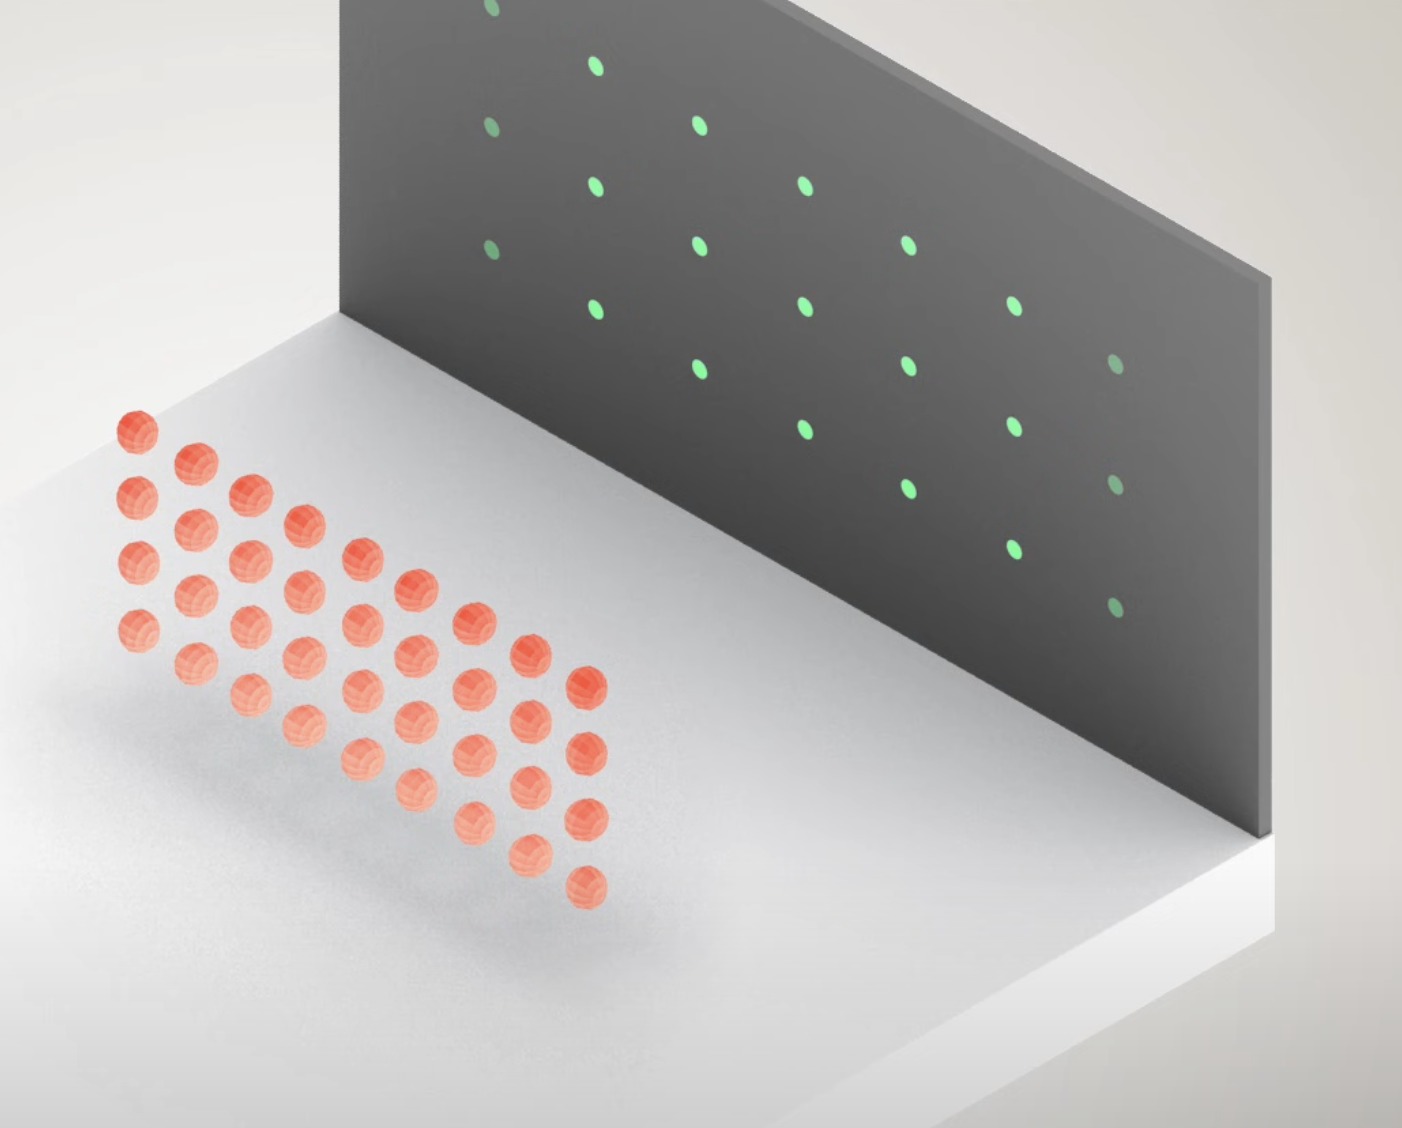
\includegraphics[scale=0.45]{Bilder/SamtaleTema4/2D-array.png}
    \caption{2D-array som produserer interferens i et gitter mønster}
    \label{fig:2d-array}
\end{figure}

\autoref{fig:2d-array} viser et 2D-gitter som får røntgen stråling på seg, på veggen danner det seg et gitter. Dette gitteret ser ut til å ha større avstand mellom punktene enn 2D-gitteret. Det vi ser på veggen er en avbildning av det resiproke rommet! Så dersom avstanden $a$ er mindre enn $1m$ vil avstanden i det resiproke rommet være større, når $a$ øker vil avstanden i reelt rom øke, og avstanden i resiprokt rom minke, husk at forholdet er invers proporsjonalt.

\begin{figure}[!htb]
    \centering
    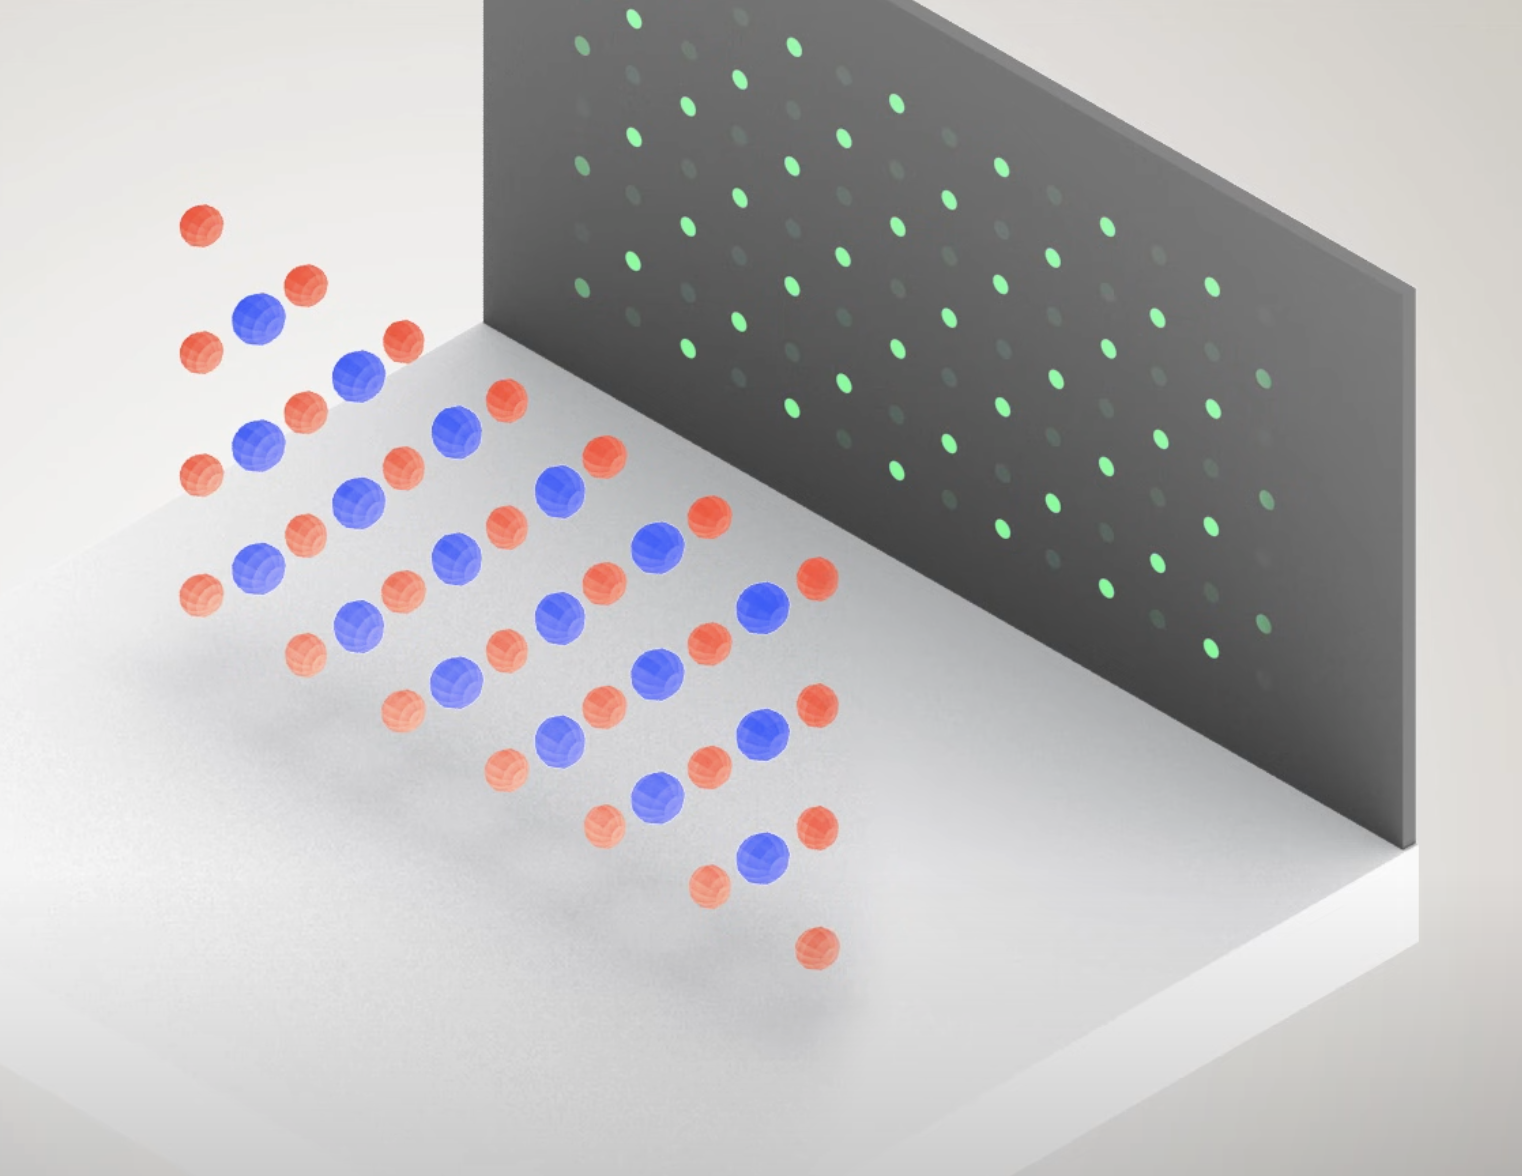
\includegraphics[scale=0.42]{Bilder/SamtaleTema4/skrot.png}
    \caption{Tilegg av atomer mellom gitterpunkt, bevarer periodisitet.}
    \label{fig:periodisity}
\end{figure}

I \autoref{fig:periodisity} er det lagt til atomer mellom gitterpunktene, men uten at de ødelegger krystallens periodisitet. Dette produserer fortsatt de samme interferenspunktene, men det varierer intensiteten.

NB! Som nevnt tidligere er mønsteret som produseres på veggen det gitteret som oppstår i det resiproke rommet. Ved å måle dette kan vi hvordan atomene i faste stoff er organisert.

Resiprokt rom er nyttig for å beskrive hva slags bølger som matcher med en gitt krystall. X-ray-diffraksjon og braggs lov kan brukes for å finne posisjon/avstand mellom atomene:

\begin{figure}[!htb]
    \centering
    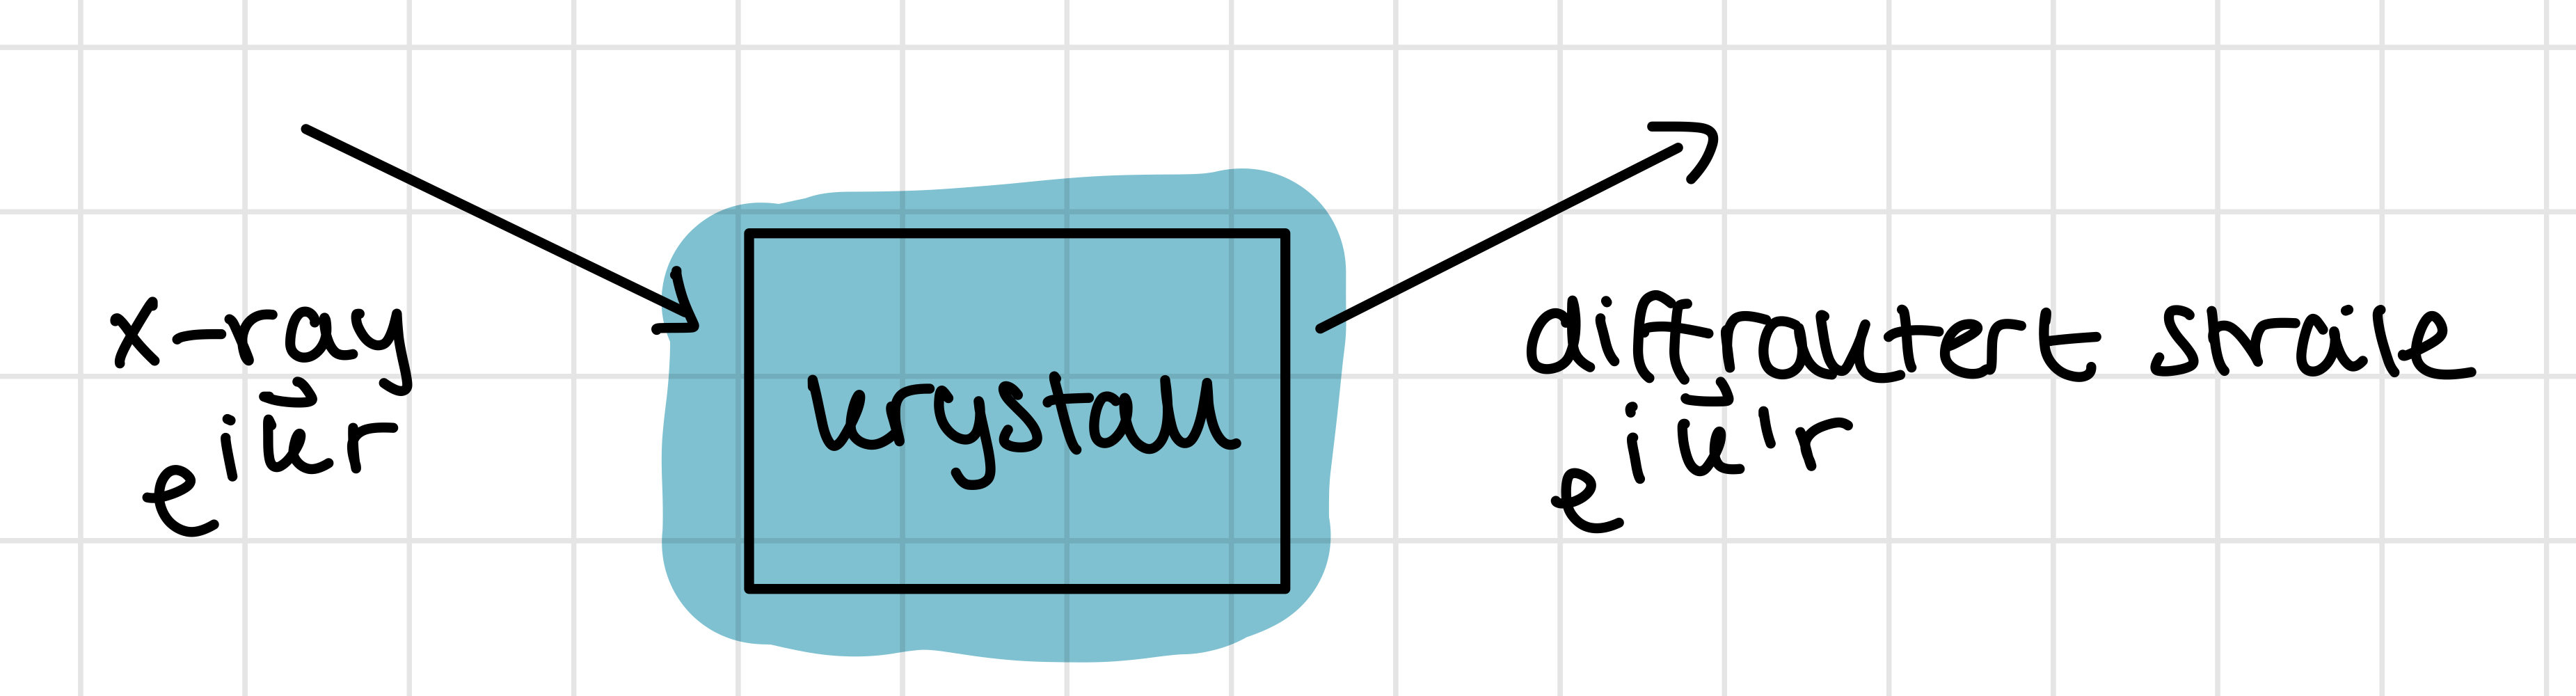
\includegraphics[scale=0.1]{Bilder/SamtaleTema4/diffraksjon.jpeg}
    \caption{Ved å skyte røntgen stråling på en krystall vil man produsere en diffraktert stråle}
    \label{fig:diffrak}
\end{figure}

For å oppnå konstruktiv interferens vil vi trenge at braggs lov er oppfylt, det vil si at ligning \ref{eq:braggs} er oppfylt.

\begin{equation}
\label{eq:braggs}
    2dsin(\theta)= n\lambda
\end{equation}

Det er også betingelser for den diffrakterte strålen, diffraksjon vil kun oppstå når 

\begin{equation}
    \Delta\Vec{k} = \Vec{k'}-\Vec{k} = \Vec{G}
\end{equation}

eller

\begin{equation}
    2\Vec{k}\cdot\Vec{G} = |\Vec{G}|^2
\end{equation}

Brillouisonen er den resiproke versjonen av Wigner-Seits cellen fra reelt rom. Planene vi som dannes mellom to Brillouisoner kalles bragg-plan. Dersom en bølge med riktig bølgelengde treffer dette planet, vil det oppstå konstruktiv interferens.

\newpage



\section{Tema 5: Kronig-Penney Modellen}
\label{tema5}

\begin{table}[!htb]
    \centering
    \caption{Samtale punkter tema 4}
    \begin{tabular}{|c|c|c|r|}
      \hline
      1 & Kronig-Penney Modellen \& Forenklinger &  \autoref{sec:tema5_1} & \cellcolor{blue}\quad\quad \\
      \hline 
      2 & Bloch's teorem & \autoref{sec:tema5_3} & \cellcolor{blue} \\
      \hline
      3 & Løsningene til Kronig-Penney Modellen & \autoref{sec:tema5_4} & \cellcolor{blue} \\
      \hline 
      4 & Dispersjonsrelasjonen, E(k) & \autoref{sec:tema5_5} & \cellcolor{blue} \\
      \hline
      5 & Effektiv masse & \autoref{sec:tema5_6} & \cellcolor{blue} \\ 
      \hline
    \end{tabular}
    \label{tab:samtalePunkt_tema1}
\end{table}

\subsection{Kronig-Penney Modellen \& Forenklinger}
\label{sec:tema5_1}
Vi begynner å nærme oss gode representasjoner av atomer nå, men vi vil gjerne kunne modulere stoff. Dette gjelder også halvledere. Potensialet mellom en proton/nøytron kjerne og et elektron kan modelleres som et coulomb potensial. Dersom man ønsker å løse SL innenfor en rimelig tid, bruker man heller en forenklet modell. Denne modellen heter Kronig-Penney modellen, visualisert i figur \ref{fig:KP}

\begin{figure}[!htb]
    \centering
    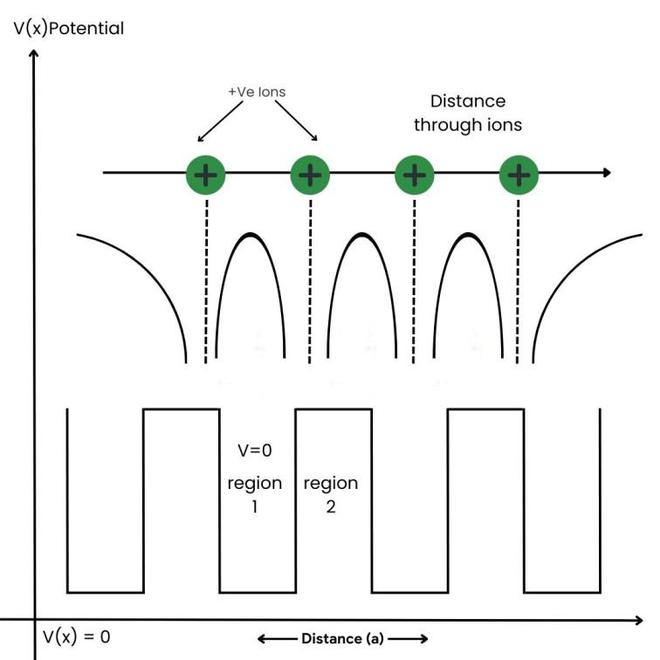
\includegraphics[scale=0.4]{Bilder/SamtaleTema5/kronigPenney.jpeg}
    \caption{Kronig-Penney modellen}
    \label{fig:KP}
\end{figure}

Ved å ta i bruk kvantebrønner kan man modellere atomer til en viss grad, energinivåene som dukker opp i brønnen tar rollen til elektronskallene. Den andre forenklingen Kronig-Penney modellen gjør er å produsere et uendelig langt gitter, dette gjør at man slipper å bry seg om rand tilfeller.

La oss se på to atomer først, dette vil virke som en dobbel kvantebrønn, slik som vi så på i \autoref{sec:tema3_7}. Om avstanden mellom de to brønnene er store, vil de i essens virke sm to uavhengige brønner. Men dersom de er nærme nok vil vi få en splitting av energinivåer (bonding nederst, og anti-bonding øvest). Splittingen blir større og større jo høyere energinivå vi har, det blir mer og mer lekkasje. 

Det er verdt å merke seg at antall energinivåer per bånd, er lik antall brønner som igjen er lik antall lineære kombinasjoner i.e. løsninger av SL. Her kommer den store nedsiden av Kronig-Penney modellen, det at det er uendelig mange brønner gjør at energien i hvert bånd er kontinuerlig, selvom det brude vært diskret.

Når vi beveger oss oppover brønnen vil det være større avstand mellom energinivåene i et bånd. Dette er fordi det er mer og mer lekkasje desto nærmere man kommer $V_0$.

\subsection{Bloch's teorem}
\label{sec:tema5_3}
Bloch's teorem sier at løsningen på SL i et periodisk potensial $V(x)$, kan uttrykket ved plane bølger modulert av en periodisk funksjon. Matematisk er det uttrykket som 

\begin{empheq}[box=\tcbhighmath]{align}
    \label{eq:bloch}
    \psi(x) = e^{ik\textbf{r}}u(\textbf{r})
\end{empheq}

Her er da $e^{ik\textbf{r}}$ planbølgen, og $u(\textbf{r})$ er en vilkårlig funksjon med samme periodisitet som krystallen. \autoref{fig:bloch} gir en visuell representasjon av ligning \ref{eq:bloch}.

\begin{figure}[!htb]
    \centering
    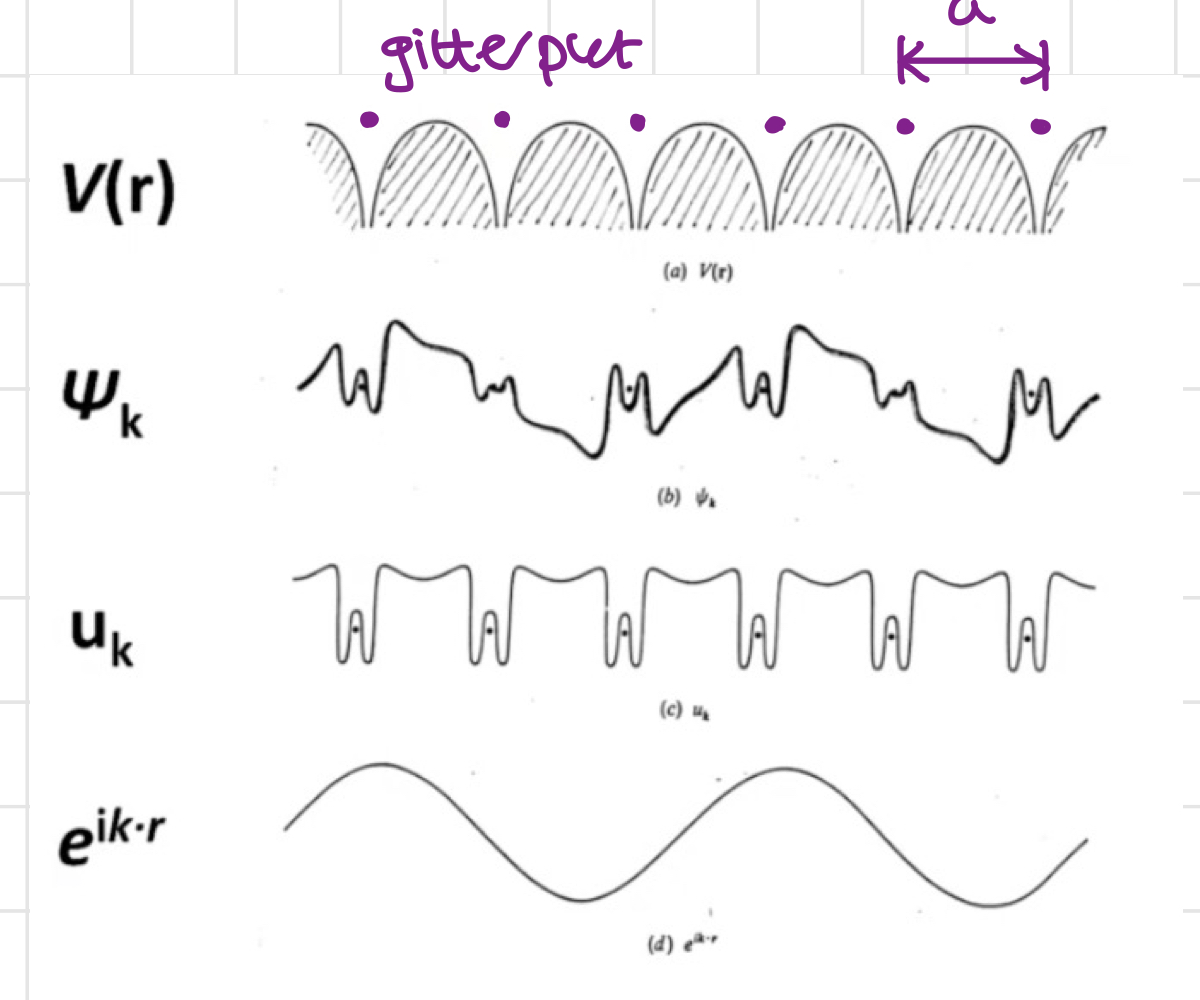
\includegraphics[scale=0.29]{Bilder/SamtaleTema5/blochs.jpeg}
    \caption{Øverst har vi potensialet til en perfekt krystall $V(\textbf{r})$. Under har vi bølgefunksjonen, denne kan dekomponeres inn i et produkt bestående av den stående bølgen nederst, og den periodiske funksjonen $u_k(\textbf{r})$ smo har samme periodisitet som $V(\textbf{r})$.}
    \label{fig:bloch}
\end{figure}

\subsection{Løsningene til Kronig-Penney Modellen}
\label{sec:tema5_4}
Utledningen av løsningen til KP-modellen er krunglette og lang og er heller ikke pensum, men resultatet av modellen er. \autoref{eq:solKP} gir en forenklet løsning av KP-modellen, men nok til å hente ut informasjonen vi trenger for å se på dispersjonsrelasjonen.

\begin{equation}
    \label{eq:solKP}
    cos(...) = sin(...)cos(..)...+cosh(...)
\end{equation}

Vi ser fra ligning \ref{eq:solKP} at vi kun kan ha løsninger mellom $-1$ og $1$. 

\begin{figure}[!htb]
    \centering
    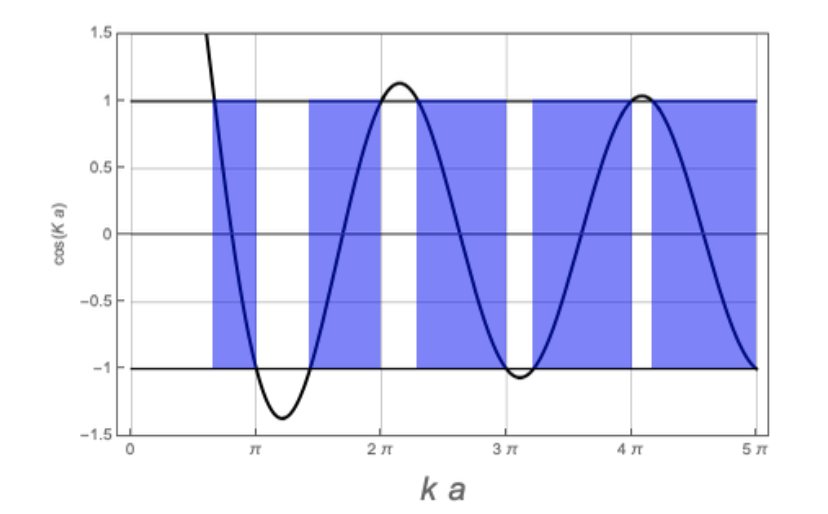
\includegraphics[scale=0.8]{Bilder/SamtaleTema5/KP-plot.png}
    \caption{Grafisk løsningen av Kronig-Penney modellen }
    \label{fig:plot-kp}
\end{figure}

$x$-aksen i dette tilfellet er en dimensjonsløs verdi som er proporsjonal med energien. Dersom vi projiserer de gyldige områdene ned på $x$-aksen og legger det oppå dispersjonslerasjonen for en fri partikkel vil vi få dispersjonsrelasjonen for Kronig-Penney modellen.

\subsection{Dispersjonsrelasjonen, E(k)}
\label{sec:tema5_5}
Som vi nevnte i slutten av \autoref{sec:tema5_4}, kan vi dersom vi legger løsningen på Kronig-Penney modellen oppå fri elektron dispersjonsrelasjonen, få ut figur \ref{fig:dispRel}

\begin{figure}[!htb]
    \centering
    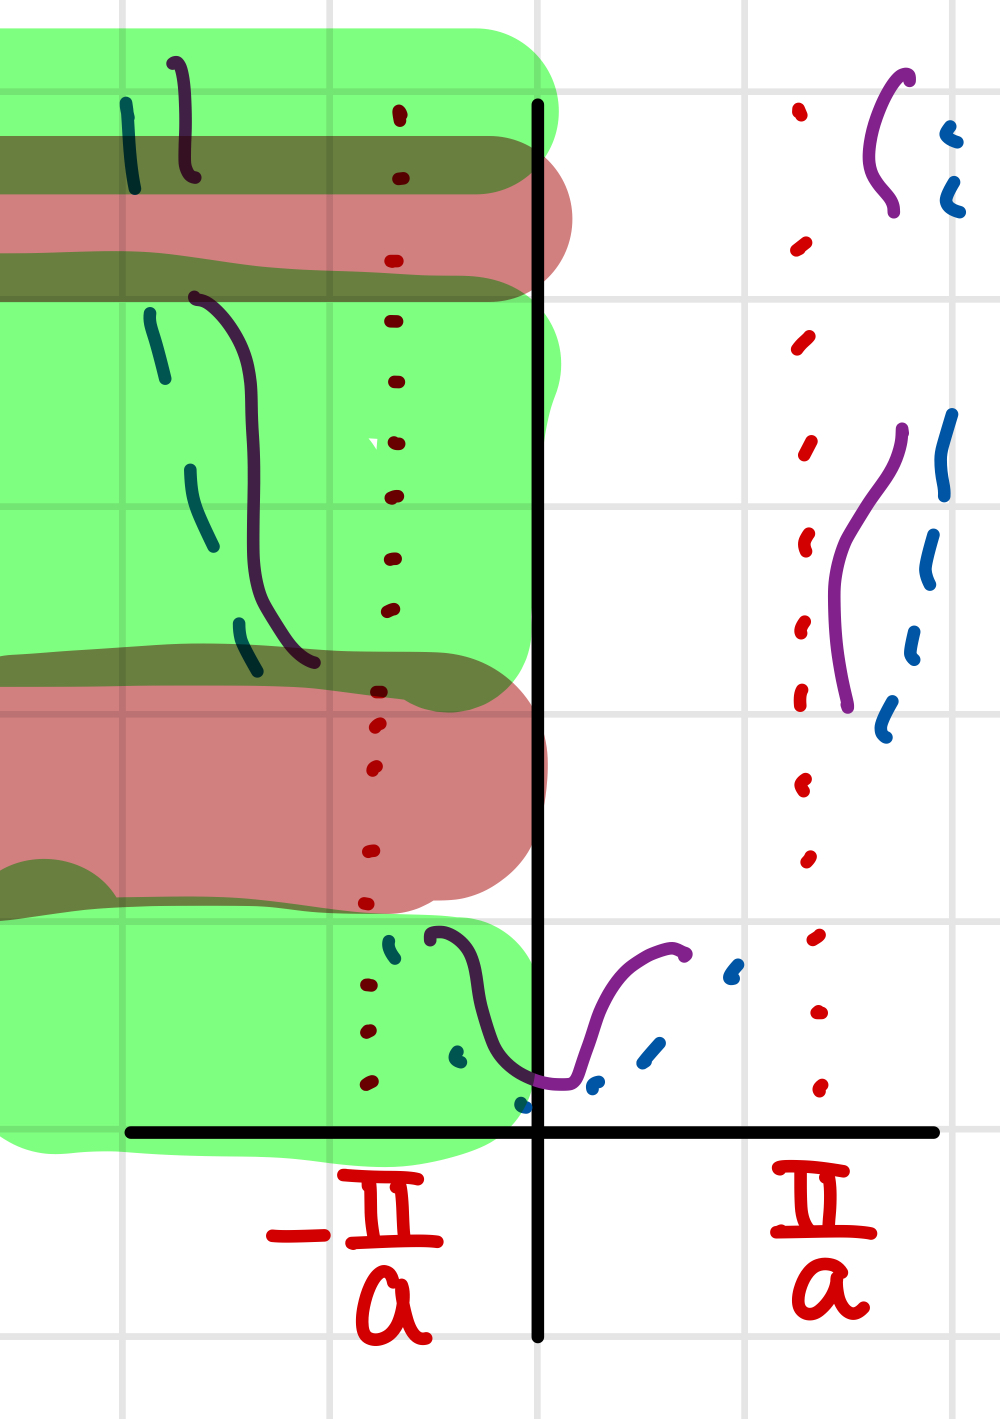
\includegraphics[scale=0.2]{Bilder/SamtaleTema5/disp-relasjon-KP.jpeg}
    \caption{Dispersjonsrelasjonen for Kronig-Penney modellen.}
    \label{fig:dispRel}
\end{figure}

Her er de grønne områdene tillate områder, disse er avhengige bølgetallet $k$ og gitterkonstanten $a$. Ved Brillouinsone grensene vil det oppstå båndgap, dette er da ved $k=\pm\frac{n\pi}{a}$.

Vi husker fra tidligere at en Brillouinsone er Wigner-Seitz cellen, men i det resiproke rom. Brillouinsonene er viktige fordi det er en representasjon av verdiene til $k$ i planbølgen som oppfyller blochs teorem.

Ved brillouinsonegrensene vil det oppstå interferens, da den reflekterte bølgen interfereres med den innkommende bølgen. Dette medfører at vi har stående bølger, og ikke kan ha energinivåer som ligger på $k = \frac{n\pi}{a}$.

Alle punkt på den lilla kurven svarer til bølgefunksjoner med bestemte k-verdier. $k$-ene er $k$-en i blochbølger ($\psi(x)=exp(ikx)u(x), \quad u(x)=u(x+a)$.

Bølger som ligger på positiv $k$-akse svarer til vandrende bølger som beveger seg i positiv $k$-retning, og det er som nevnt tidligere akkurat ved brillouinsonene at vi har betingelser som gir oss stående bølger.

$k$-en fra figur \ref{fig:dispRel} er relatert til krystallbevegelsesmengden.
\begin{equation*}
    p_{krystall} = \hbar k,
\end{equation*}

Bevegelsesmengden til det samlede systemet, dette innebærer da elektron pluss krystall. Det viser seg at $p_{krystall}$ relaterer tett til gruppehastigheten $v_g$ og er derfor et bra mål på hvordan elektron-bølgepakker beveger seg gjennom krystallen. En tilstand med postive $k$ verdier beskriver et elektron $e^-$ som beveger seg i positiv $x$-retning og andre veien for $k<0$.

Finnes flere måter å representere dispersjonsrelasjonen. \autoref{fig:reduced} viser et reduced-zone-scheme, den fra figur \ref{fig:dispRel} kalles for et extended-zone-scheme.

\begin{figure}[!htb]
    \centering
    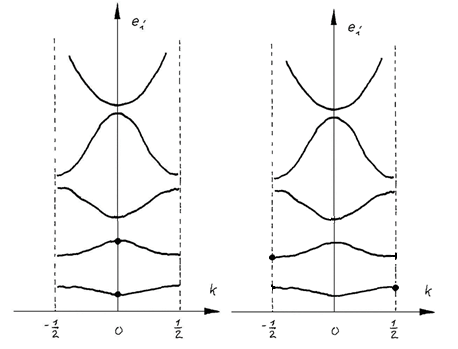
\includegraphics[scale=0.6]{Bilder/SamtaleTema5/Reduced-zone-scheme.png}
    \caption{Reduced-Zone-Scheme.}
    \label{fig:reduced}
\end{figure}

\subsection{Effektiv masse}
\label{sec:tema5_6}
Det er gunstig å kunne si noe om massen, men som vi ser fra uttrykket for energi i ligning \ref{eq:Engi} og dispersjonsrelasjonen, vil energien til en partikkel forandre seg.

\begin{equation}
\label{eq:Engi}
    E = \frac{\hbar^2k^2}{2m}
\end{equation}

Hadde vi løst ligning \ref{eq:Engi} mhp. massen, ville massen $m$ påvirkes avhengig av energien (bølgetallet $k$). Dersom vi dobbeltderiverer mhp. $k$ ser vi et forenklet uttrykk,

\begin{equation}
    \label{eq:effectiveMass}
    \begin{split}
        E &= \frac{d^2}{d k^2} \frac{\hbar^2k^2}{2m}\\
        m^* &= \frac{\hbar^2}{\frac{d^2E}{dk^2}}
    \end{split}
\end{equation}

Den effektive massen korrigerer for kreftene som virker på elektronet fra krystallen. 

Effektiv masse påvirker DOS i energi bånd, Den er med på å avgjøre hvor mange tilgjengelige tilstander det er for et gitt energinivå.

I en halvleder, så påvirker effektivmassen mobiliteten til elektronene. En lav effektiv masse gjør at elektronene er mer mobiler, og leder da strøm bedre. Kurvaturen til bånddiagrammet sier oss da noe om mobiliteten, siden den effektive massen er omvendt proporsjonal med den dobbelderiverte av energien mhp. $k$, vil en større kurvatur i  dispersjonsrelasjonen gi høyere mobilitet.

\section{Tema 6: Båndstruktur}
\label{tema6}


\begin{table}[!htb]
    \centering
    \caption{Samtale punkter tema 4}
    \begin{tabular}{|c|c|c|r|}
      \hline 
      1 & Fermi-Dirac fordelingen \& Båndstruktur i 1. Brilouisone & \autoref{sec:tema6_2} & \quad\quad \cellcolor{blue} \\
      \hline
      2 & Tilstandstetthet (DOS) & \autoref{sec:tema6_3} & \cellcolor{red} \\
      \hline
      3 & Elektron og hull i båndsrukturen & \autoref{sec:tema6_4} & \cellcolor{blue} \\
      \hline 
      4 & Båndstruktur i 3D & \autoref{sec:tema6_5} & \cellcolor{blue} \\
      \hline
      5 & Direkte og indirekte båndgap & \autoref{sec:tema6_6} & \cellcolor{blue} \\ 
      \hline
      6 & Forenklet bånddiagram & \autoref{sec:tema6_7} & \cellcolor{blue} \\
      \hline
    \end{tabular}
    \label{tab:samtalePunkt_tema1}
\end{table}


\subsection{Fermi-Dirac fordelingen \& Båndstruktur i 1. Brilouisone}
\label{sec:tema6_2}
Første Brillouinsone inneholder all informasjon vi trenger for elektroner i en krystall. En avbildning er illustrert i figur \ref{fig:infoBD}. Kurvene er ikke kontinuerlige, og sirkelene som er tegnet representerer elektroner, de ligger som ''perler på en snor''. 

\begin{figure}[!htb]
    \centering
    \includegraphics[scale=0.2]{Bilder/SamtaleTema6/infoBD.jpeg}
    \caption{1. Brillouin sone med elektroner tegnet på.}
    \label{fig:infoBD}
\end{figure}

NB! Det er $2N$ tilstander i hvert bånd, $N$ er antall energinivåer, og dette multipliseres med to siden det er mulig å ha spinn opp og spinn ned elektroner per energinivå.

En annen forklaring er at dette er elektroniske tilstander som alle har ulik $k$-verdi. Dette er Bloch bølger $\psi(x)=exp(ikx)u(x)$. Hvor $u$ har samme periodisitet som krystallen. 

Grunnen til vi velger å bruke elektroniske tilstander istedet for elektron er fordi man ved bruk av terminologien tar hensyn til den komplekse naturen til elektronets bevegelse i fast stoff. Elektroniske tilstander forklarer ikke bare den romlige posisjonen til elektron, men sier også noe om energi.

Eksempler på ulike elektroniske tilstander med ulik $k$-verdier kan være: 

\textbf{Valensbåndet}: Elektroniske tilstander nær bunnen av valensbåndet representerer tilstander der elektroner har lav energi ($k$ er liten, stor $\lambda$) og er bundet til kjernen.

\textbf{Ledningsbåndet}: Elektroniske tilstander nær toppen av ledningsbåndet har ulike $k$-verdier og representerer tilstander der elektronene har høy energi og er relativt fri til å bevege seg fritt gjennom krystallen.

Fra figur \ref{fig:infoBD} ser vi $E_F$, dette er fermienergien. Fermienergien forteller oss at ved $\SI{0}{\kelvin}$ er alle tilstander over $E_F$ tomme, mens alle tilstander under $E_F$ er fyllt opp, dette er fordi ved $\SI{0}{\kelvin}$ er det ingen termisk energi tilstedet. Vi kan ved bruk av dette produsere en sannsynlighetsfordeling for hvor vi kan finne elektroner.

\textbf{Fermi-Dirac-fordelingen} er en sannsynlighetsfordeling som beskriver uskarpheten ved fylling av tilstander.

\begin{empheq}[box=\tcbhighmath]{align}
    \label{eq:fermi-dirac}
    f(E) = \frac{1}{1+e^{\frac{(E-E_F)}{k_{b}T}}}
\end{empheq}

Funksjonen består av $k_b$ som er boltzmanns konstant, $T$ er temperaturen til krystallen. $E_F$ er fermienergien og $E$ er energien vi vil se om et elektron kan inneha. Denne funksjonen er da også en funksjon av temperaturen, da den produserer en helt ny sannsynlighetsfordeling. Vi ser at for $T=\SI{0}{\kelvin}$ får vi

\begin{equation}
\label{eq:potInfinite}
f(E) = \left\{
        \begin{array}{ll}
            0 & \quad E > E_F \\
            1 & \quad E < E_F
        \end{array}
    \right.
\end{equation}

Vi ser at $T=\SI{0}{\kelvin}$ er fordelingen en unit step function. \autoref{fig:fermiDirac} viser Fermi-Dirac fordelingen ved forskjellige temperaturer $T$.

\begin{figure}[!htb]
    \centering
    \includegraphics[scale=0.8]{Bilder/SamtaleTema6/fermiDirac.png}
    \caption{Fermi-Dirac fordelingen ved forskjellige temperaturer.}
    \label{fig:fermiDirac}
\end{figure}

La oss ta et eksempel der vi har to materialer, det ene har $E_F$ mot det øvre delen av valens båndet, som vi kaller det mat. \textcircled{1}, det andre har $E_F$ midt mellom valens bånd og ledningsbånd, vi kaller dette for mat. \textcircled{2}.

\textcircled{1} og \textcircled{2} kommer til å oppføre seg veldig forskjellig. \autoref{fig:sammenligning} viser de to materialene. ser vi på $x$-aksen har man ulike $k$, dette har noe med bevegelsesmengden å gjøre (husk at dette er krystall bevegelselsesmengden). Elektronene på positiv side har bevegelsesmengde i positiv $k$-retning, og dette handler om gruppehastigheten til Blochbølgene.

\begin{figure}[!htb]
    \centering
    \includegraphics[scale=0.2]{Bilder/SamtaleTema6/sammenligning.jpeg}
    \caption{Venstre har vi mat. \textcircled{1}, og til høyre har vi mat. \textcircled{2}.}
    \label{fig:sammenligning}
\end{figure}

Et eksempel på mat. \textcircled{2} er silisium, de elektronene med bevegelsesmengde i positiv $k$-retning representerer bølgepakker/elektroner som beveger seg inni silisiumkrystallen. Desto større bevegelsesmengde, jo lengre unne origo er elektronet (større $k$), tilsvarende for elektroner i negativ $k$-retning, men da med negative fortegn.

\newpage
For mat. \textcircled{1} ser vi at båndstrukturen er usymetrisk, dette medfører til at netto bevegelselmengde ikke er null

\begin{equation*}
    \sum_i^N p_i \neq 0, 
\end{equation*}

Dersom båndene var like fulle på begge sider av $k=0$, slik som i mat. \textcircled{2}, får vi 

\begin{equation*}
    \sum_i^N p_i = 0, 
\end{equation*}

Dette gir en netto null ladningstransport. Vi kan med det si at mat. \textcircled{1} leder strøm bra, og vi kan si det er et metallisk materiale. Mat. \textcircled{2} leder ikke strøm bra, og vi kan si det oppfører seg som en isolator i utgangspunktet. Om båndgapet ikke er for stort kan vi si det er halvleder, dette er fordi det ikke krever veldig mye for et elektron å ''hoppe'' opp i ledningsbåndet.

\subsection{Tilstandstetthet (DOS)}
\label{sec:tema6_3}
Fylling av båndstrukturen er avgjørende for et materrial sine elektriske egenskaper

Metaller har halvfulle bånd, og leder derfor strøm godt. Isolatorer har fulle valens bånd, og tomme ledningsbånd og leder derfor ikke strøm. Vi er interessert i halvledere (som silisium). I utgangspunktet så har de fulle valensbånd, og tomme ledningsbånd, men det kreves lite energi for å overføre noen $e^-$fra øverste fylte båndt (VBM) til CBM. Det er slik silisium oppnår ledningsevne.

Så elektroner i ledgningsbåndet er det som kan gi ladningstransport. Det kan også være ''hullene'' som er i valensbåndet.

Vi er interessert i tallet på $e^-$ som er i CB, og antall hull i VB. For å finne disse, må vi koombinere informasjon fra båndstrukturen og Fermi-Dirac fordelingen. Ved å telle opp produktet av tilgjengelig plass og sannsynligheten for at denne er fylt, dette gir oss følgende integral.

\begin{equation}
    n(E) = \int_{0}^{\infty} g(E) \cdot f(E) dE
\end{equation}

$n(E)$ forteller os tettheten av $e^-$ i CB. Vi integrerer over alle mulige energinivå, $g(E)$ er density of states, denne funksjonen gir oss tettheten av tilstander for en viss energi. og $f(E)$ er sannsynligheten for å finne et elektron gitt en hvis energi.

I et båndgap er $g(E)=0$, fordi det ikke finnes noen mulige tilstander i båndgapet. Verdien på $g(E)$ avhenger av hvor tett elektronene ligger langs $k$-aksen. Vi antar at formen på båndene er parabler, dette er ikke en spesielt god antakelse, men den er god nok i de ''spennende'' områdene. 

Hvor tett tilstandene ligger, avhenger av krystallen. Man kan se dette ved hjelp av to metoder, begge gir samme $g(E)$ til slutt.

La oss anta at vi har en krystall som er rektangulær, med sider $L_x,L_y$ og $L_z$ og volum $V=L_xL_yL_z$. Med periodiske grensebetingelser får vi 

\begin{equation*}
    \psi(x+L_x,y,z) = \psi(x,y+L_y,z) = \psi(x,y,z+L_z) = \psi(x,y,z)
\end{equation*}

Setter vi dette inn i blochs toerem får vi

\begin{equation*}
    \exp{ik_xL_x} = \exp{ik_yL_y} = \exp{ik_zL_z} = 1    
\end{equation*}

Vi vet da at produktet av $k_j$ og $L_j$ må være heltall to pi, altså

\begin{equation*}
    k_x=\frac{2\pi}{L_x}n_x, \quad k_y = \frac{2\pi}{L_y}n_y, \quad
    k_z = \frac{2\pi}{L_z}n_z
\end{equation*}

Der $n_x,n_y,n_z=0,\pm 1, ..., N$. Vi ser at disse $k_j$ene er komponenter i bølgevektoren $\Vec{k}$, og vi kan med det si at produktet av alle tre gir oss the minste volumnet i $k$-rommet.

\begin{equation*}
    \frac{(2\pi)^3}{L_xL_yL_z} = \frac{(2\pi)^3}{V}
\end{equation*}

Vi vet at det er akkurat ett gitter punkt tilstede i dette volumet, fra det kan man trekke konklusjonen at tettheten av tillatte $\Vec{k}$ er uniform og lik $\frac{V}{(2\pi)^3}$ i $k$-rommet. Dette gir oss uttrykket 

\begin{equation}
    \label{eq:kTett}
    g(\Vec{k}) = 2 \frac{V}{(2\pi)^3}
\end{equation}

der faktoren to kommer fra spinn opp spinn ned karakteristikken til elektroner. $g(\Vec{k})$ er funksjonen som forteller oss om tettheten i $k$-rommet, denne er koblet opp mot funksjonen vi ønsker å finne $g(E)$. Forholdet mellom de to kan ser ut som

\begin{equation}
    \label{eq:forhold}
    g(E)dE = g(\Vec{k})d\Vec{k}
\end{equation}

her er $dE$ og $d\Vec{k}$ små intervaller av hhv. energi og enhetsvolum i $k$-rommet. For å finne $g(E)$ må vi vite forholdet mellom energien og $k$-rommet. Vi kan ta i bruk uttrykket vi har for energi, siden vi er interessert i området som er omtrent likt en parabel. 

\begin{equation}
\label{eq:energi_utledning}
    \begin{split}
        E(\Vec{k}) &= \frac{\hbar^2 k^2}{2m^*} \\
        dE &= \frac{\hbar^2}{2m^*}(2k)dk
    \end{split}
\end{equation}

Hvis vi tar i bruk sfæriske koordinater, kan vi skrive om $d\Vec{k}$ til

\begin{equation}
    \begin{split}
        d\Vec{k} &= d \bigg( \frac{4\pi}{3}k^3\bigg) \\
        d\Vec{k} &= 4\pi k^2 dk
    \end{split}
\end{equation}

Setter vi dette resultatet inn i ligning \ref{eq:energi_utledning}, får vi 
\begin{equation}
    \label{eq:dE}
    dE = \frac{\hbar^2}{2m^*} \bigg( \frac{1}{2\pi k}\bigg) d\Vec{k}
\end{equation}

Tar vi i bruk uttrykket for energi kan vi skrive det om mhp. $k$ og sette inn i ligning \ref{eq:dE}.

\begin{equation}
\label{eq:dEFin}
    dE = \frac{1}{2\pi}\bigg(
    \frac{\hbar^2}{2m^*}\bigg)^{\frac{3}{2}}
    \frac{1}{\sqrt{E}} d\Vec{k}
\end{equation}

Setter vi inn ligning \ref{eq:forhold} får vi 

\begin{equation}
    \label{eq:5.39.2}
    g(E) = 2\pi \bigg(
    \frac{2m^*}{\hbar^2} \bigg)^{\frac{3}{2}} \sqrt{E}g(\Vec{k})
\end{equation}

og ved å ta i bruk ligning \ref{eq:kTett} ender vi med

\begin{equation}
    \label{eq:tetthetFunc}
    g(E) = \frac{V}{2\pi^2}\bigg(\frac{2m^*}{\hbar^2}\bigg)^{\frac{3}{2}} \sqrt{E}
\end{equation}

Vi definerer ofte $g(E)=0$ ved ferminivået. Ferminivået er det interessante området der materialer går mellom ikke-ledende og ledende.

\begin{figure}[!htb]
    \centering
    \subfloat[\centering Tilstandstetthen \ref{eq:even}]{{\includegraphics[width=7cm]{Bilder/SamtaleTema6/dosgraf.jpeg} }}%
    \qquad
    \subfloat[\centering $g(E)\cdot f(E)$ \ref{eq:odd}]{{\includegraphics[width=7cm]{Bilder/SamtaleTema6/g(E)f(E).jpeg} }}%
    \caption{Tilstandstettheten $g(E)$ til venstre, og produktet av tilstandstetthen og Fermi-Dirac til høyre}%
    \label{fig:dobbelgreie}%
\end{figure}

\begin{figure}[!htb]
    \centering
    \includegraphics[scale=1.5]{Bilder/SamtaleTema6/DOS.png}
    \caption{Tilstandstettheten(DOS) for silisium på venstre side, plotet sammen med bånd diagrammet.}
    \label{fig:DOS_plot}
\end{figure}


Vi ser fra figur \ref{fig:dobbelgreie} at produktet av fermi-dirac fordelingen og tilstandstettheten avtar relativt raskt, dette produktet kallses ladningsbærertettheten og forteller oss antall ladningsbærere per volum. Dette inkluderer hull i valensbåndet da dette også kan ses på som ladningsbærere.

\newpage
\subsection{Elektron og hull i båndsrukturen}
\label{sec:tema6_4}
Elektroner befinner seg i ulike energibånd i et faststoff, det høyeste energibåndet som er fylt av elektroner ved lav temperatur kalles valensbåndet. Elektroner i valensbåndet har bundne tilstander. og de bidrar ikke uten videre til elektrisk ledning. Ved påvirkning fra ytre faktorer, som f.eks spenning, kan elektroner eksiteres til høyere energier, eller opp til ledningsbåndet, her kan de bevege seg friere og bidra til elektrisk ledning.

Et hull er et fravær av et elektron i valensbåndet, det oppfører seg som en positivt ladet partikkel. Hull kan bevege seg gjennom krystallen, og de kan betraktes som positive ladningsbærere. Når et elektron hopper fra valensbåndet til ledningsbåndet, etterlater det seg hull i valensbåndet som kan bevege seg gjennom krystallen og bidra til elektrisk ledning.

\subsection{Båndstruktur i 3D}
\label{sec:tema6_5}
Tidligere i dokumentet har vi produsert situasjoner ved hjelp av to dimensjoner, en for $k$-rommet, og en for energien $E(k)$, men nå vil vi inn i 3D for å tegne ekte faststoff. Vi kan prøve å lage en 3D tegning

\begin{figure}[!htb]
    \centering
    \includegraphics[scale=0.2]{Bilder/SamtaleTema6/2d-bandstruct.jpeg}
    \caption{Forsøk på 2D tegning...}
    \label{fig:2d_tegning}
\end{figure}

\autoref{fig:2d_tegning} så ikke så ille ut, men vi må jo lage 3 av disse, en til for $(k_x,k_z)$ og en for $(k_y,k_z)$. Vi prøver derfor noe litt annet, la oss heller si at vi går i en retning i $k$-rommet istedet, og grafer dette, så i en annen retning og tegner mens vi går rundt. Dette produserer figur \ref{fig:si_band}



\begin{figure}[!htb]
    \centering
    \includegraphics[scale=0.55]{Bilder/SamtaleTema6/si_banddiagram.png}
    \caption{Silisium sitt bånddiagram.}
    \label{fig:si_band}
\end{figure}


\begin{figure}[!htb]
    \centering
    \includegraphics[scale=0.55]{Bilder/SamtaleTema6/brillouinZone.png}
    \caption{Første brillouin sone visualisert i 3D, Firkantene er flatsidene mellom to enhetsceller, sekskantene representerer bragg plan.}
    \label{fig:BZ}
\end{figure}

$\Gamma$ er sentrum, alle de greske bokstavene som dukker opp i figur \ref{fig:BZ} dukker også opp i figur \ref{fig:si_band}, dette hører med retningen de går rundt i rommet. 

\subsection{Direkte og indirekte båndgap}
\label{sec:tema6_6}
Et båndgap er avstanden mellom VBM og CBM (eller to vilkårlige bånd, men vi bryr oss om VBM og CBM).

Om $k$-vektoren til VBM er lik den i CBM, kalles det et \textit{direkte båndgap}, men om de ikke er like kalles det et \textit{indirekte båndgap}.

For direkte båndgap må krystallmomentet k (husk $p_{krystall}=\hbar k$) være likt VBM og CBM, dette gjør at elektroner i VBM kan ''hoppe'' direkte til CBM, de trenger ikke bevege seg til siden i k-rommet, altså de trenger ikke tilførsel av bevegelsesmengde. Dette kan gjøres ved tilførsel av energi i form av et foton.

For indirekte båndgap er ikke $k$-vektorene like, dette gjør at krystallmomentet i VBM og CBM er ulikt. Siden momentet er uliktt må noe av momentet til elektronet overføres til gitteret før det tar plass i CBM. For å eksitere et elektron i et indirekte båndgap, kan vi introdusere energi til systemet som kan omgjøres til bevegelsesmengde, for eksempel akkustiske bølger, dette vil produsere gitter vibrasjoner, noe som gir oss et høyere krystall moment. Elektroner inneholder ikke en stor bevegelsesmengde, så det må en kombinasjon av disse til for å eksitere ved et indirekte båndgap. 

Eksitering i et direkte båndgap gjøres ofte med fotoner, men ofte har fotoner litt mer energi enn det som egentlig trengs for eksitasjonen fra VBM til CBM, derfor frigjøres den ekstra energien ofte som fotoner. Dette gjør at halvledere med direkte båndgap egner seg godt i bruk i optiske komponenter som LED, lasere og solceller. 

\subsection{Forenklet bånddiagram}
\label{sec:tema6_7}
Forenklede bånddiagram er nyttige, det er enklere å visualisere ved å se på en diode av typen p-n, som illustrert i figur \ref{fig:p-n}

\begin{figure}[!htb]
    \centering
    \includegraphics[scale=0.2]{Bilder/SamtaleTema6/diode.jpeg}
    \caption{diode av typen p-n}
    \label{fig:p-n}
\end{figure}

Dioden består av halvleder materiale, som vi har dopet med noen urenheter. Dopingen gjør i prinsipp at vi hever ferminivået $E_F$. I p-delen ligger $E_F$ nærmest valensbåndet, og i n-delen ligger $E_F$ nærmest ledningsbåndet.

Forenklede bånddiagram plotter bare valence band max (\textbf{VBM} - toppen av valensbåndet) og conduction band min (\textbf{CBM} bunnen av ledningsbånde). Dette blir sende ut som i figur \ref{fig:forenkl}.

\begin{figure}[!htb]
    \centering
    \includegraphics[scale=0.2]{Bilder/SamtaleTema6/forenklet.jpeg}
    \caption{Forenklet bånd diagram}
    \label{fig:forenkl}
\end{figure}

Disse blir ofte slått sammen og $E_F$ blir sentrert for de to delene. Illustrasjonen i figur \ref{fig:forenkl-sammen} viser hvordan dette ser ut.

\begin{figure}[!htb]
    \centering
    \includegraphics[scale=0.2]{Bilder/SamtaleTema6/forenklet-sentrert.jpeg}
    \caption{Forenklet bånddiagram med sentrert $E_F$}
    \label{fig:forenkl-sammen}
\end{figure}

%Bibliografi
\newpage

\phantomsection
\addcontentsline{toc}{section}{Referanser}
\begin{thebibliography}{99}

\printbibliography{}

\end{thebibliography}


%Tillegg
%Tillegg. Flere tillegg legges til ved å lage flere sections:-----------------
\appendix

\section{Kvantemekanisk Notasjon}
\label{notasjon}

Kvantemekanikken introduserer notasjon som kan være utfordrende, appendixen forsøker å gi en oversikt over de ulike notasjonene og deres bruksområder.

\begin{equation*}
    \bra{} -> \text{'bra'}
\end{equation*}

\begin{equation*}
    \ket{} -> \text{'ket'}
\end{equation*}

\begin{equation*}
    \bra{n} -> \text{'bra vektor'} = \psi_n^*(x)
\end{equation*}

\begin{equation*}
    \ket{n} -> \text{'ket vektor'} = \psi_n(x)
\end{equation*}

\begin{equation*}
    \bra{m}\ket{n} = \int_{-\infty}^{\infty}\psi_m^*\psi_n \quad \text{'overlapp integral'}
\end{equation*}

\begin{equation*}
    \bra{m}\hat{A}\ket{n} = \int_{-\infty}^{\infty}\psi_m^*\hat{A}\psi_n \quad \text{'matrise element'}
\end{equation*}

\begin{equation*}
    \bra{n}\ket{n} = \int_{-\infty}^{\infty}\psi_n^*\psi_n \quad \text{= 1 for normalisert }\psi
\end{equation*}

\begin{equation*}
    \bra{n}\hat{A}\ket{n} = \int_{-\infty}^{\infty}\psi_n^*\hat{A}\psi_n = <\hat{A}> \quad \text{Forventningsvedien til }\hat{A}
\end{equation*}

\begin{equation*}
<\hat{A}> = \frac{\bra{n}\hat{A}\ket{n}}{\bra{n}\ket{n}} \text{Forventningsverdi med normalisering}
\end{equation*}



\end{document}